\documentclass[twoside]{book}

% Packages required by doxygen
\usepackage{fixltx2e}
\usepackage{calc}
\usepackage{doxygen}
\usepackage{graphicx}
\usepackage[utf8]{inputenc}
\usepackage{makeidx}
\usepackage{multicol}
\usepackage{multirow}
\PassOptionsToPackage{warn}{textcomp}
\usepackage{textcomp}
\usepackage[nointegrals]{wasysym}
\usepackage[table]{xcolor}

% Font selection
\usepackage[T1]{fontenc}
\usepackage{mathptmx}
\usepackage[scaled=.90]{helvet}
\usepackage{courier}
\usepackage{amssymb}
\usepackage{sectsty}
\renewcommand{\familydefault}{\sfdefault}
\allsectionsfont{%
  \fontseries{bc}\selectfont%
  \color{darkgray}%
}
\renewcommand{\DoxyLabelFont}{%
  \fontseries{bc}\selectfont%
  \color{darkgray}%
}
\newcommand{\+}{\discretionary{\mbox{\scriptsize$\hookleftarrow$}}{}{}}

% Page & text layout
\usepackage{geometry}
\geometry{%
  a4paper,%
  top=2.5cm,%
  bottom=2.5cm,%
  left=2.5cm,%
  right=2.5cm%
}
\tolerance=750
\hfuzz=15pt
\hbadness=750
\setlength{\emergencystretch}{15pt}
\setlength{\parindent}{0cm}
\setlength{\parskip}{0.2cm}
\makeatletter
\renewcommand{\paragraph}{%
  \@startsection{paragraph}{4}{0ex}{-1.0ex}{1.0ex}{%
    \normalfont\normalsize\bfseries\SS@parafont%
  }%
}
\renewcommand{\subparagraph}{%
  \@startsection{subparagraph}{5}{0ex}{-1.0ex}{1.0ex}{%
    \normalfont\normalsize\bfseries\SS@subparafont%
  }%
}
\makeatother

% Headers & footers
\usepackage{fancyhdr}
\pagestyle{fancyplain}
\fancyhead[LE]{\fancyplain{}{\bfseries\thepage}}
\fancyhead[CE]{\fancyplain{}{}}
\fancyhead[RE]{\fancyplain{}{\bfseries\leftmark}}
\fancyhead[LO]{\fancyplain{}{\bfseries\rightmark}}
\fancyhead[CO]{\fancyplain{}{}}
\fancyhead[RO]{\fancyplain{}{\bfseries\thepage}}
\fancyfoot[LE]{\fancyplain{}{}}
\fancyfoot[CE]{\fancyplain{}{}}
\fancyfoot[RE]{\fancyplain{}{\bfseries\scriptsize Generated on Mon Jan 5 2015 02\+:14\+:08 for Jamie Slowgrove -\/ P\+G\+G Assignment 1 -\/ S\+D\+L by Doxygen }}
\fancyfoot[LO]{\fancyplain{}{\bfseries\scriptsize Generated on Mon Jan 5 2015 02\+:14\+:08 for Jamie Slowgrove -\/ P\+G\+G Assignment 1 -\/ S\+D\+L by Doxygen }}
\fancyfoot[CO]{\fancyplain{}{}}
\fancyfoot[RO]{\fancyplain{}{}}
\renewcommand{\footrulewidth}{0.4pt}
\renewcommand{\chaptermark}[1]{%
  \markboth{#1}{}%
}
\renewcommand{\sectionmark}[1]{%
  \markright{\thesection\ #1}%
}

% Indices & bibliography
\usepackage{natbib}
\usepackage[titles]{tocloft}
\setcounter{tocdepth}{3}
\setcounter{secnumdepth}{5}
\makeindex

% Hyperlinks (required, but should be loaded last)
\usepackage{ifpdf}
\ifpdf
  \usepackage[pdftex,pagebackref=true]{hyperref}
\else
  \usepackage[ps2pdf,pagebackref=true]{hyperref}
\fi
\hypersetup{%
  colorlinks=true,%
  linkcolor=blue,%
  citecolor=blue,%
  unicode%
}

% Custom commands
\newcommand{\clearemptydoublepage}{%
  \newpage{\pagestyle{empty}\cleardoublepage}%
}


%===== C O N T E N T S =====

\begin{document}

% Titlepage & ToC
\hypersetup{pageanchor=false,
             bookmarks=true,
             bookmarksnumbered=true,
             pdfencoding=unicode
            }
\pagenumbering{roman}
\begin{titlepage}
\vspace*{7cm}
\begin{center}%
{\Large Jamie Slowgrove -\/ P\+G\+G Assignment 1 -\/ S\+D\+L }\\
\vspace*{1cm}
{\large Generated by Doxygen 1.8.8}\\
\vspace*{0.5cm}
{\small Mon Jan 5 2015 02:14:08}\\
\end{center}
\end{titlepage}
\clearemptydoublepage
\tableofcontents
\clearemptydoublepage
\pagenumbering{arabic}
\hypersetup{pageanchor=true}

%--- Begin generated contents ---
\chapter{Hierarchical Index}
\section{Class Hierarchy}
This inheritance list is sorted roughly, but not completely, alphabetically\+:\begin{DoxyCompactList}
\item \contentsline{section}{Entity}{\pageref{class_entity}}{}
\begin{DoxyCompactList}
\item \contentsline{section}{Background}{\pageref{class_background}}{}
\item \contentsline{section}{Creature}{\pageref{class_creature}}{}
\begin{DoxyCompactList}
\item \contentsline{section}{Enemy}{\pageref{class_enemy}}{}
\item \contentsline{section}{Player}{\pageref{class_player}}{}
\end{DoxyCompactList}
\item \contentsline{section}{Map\+Object}{\pageref{class_map_object}}{}
\begin{DoxyCompactList}
\item \contentsline{section}{Block}{\pageref{class_block}}{}
\item \contentsline{section}{Gem}{\pageref{class_gem}}{}
\end{DoxyCompactList}
\end{DoxyCompactList}
\item \contentsline{section}{Map\+Loader}{\pageref{class_map_loader}}{}
\item \contentsline{section}{State}{\pageref{class_state}}{}
\begin{DoxyCompactList}
\item \contentsline{section}{Game\+State}{\pageref{class_game_state}}{}
\item \contentsline{section}{Menu\+State}{\pageref{class_menu_state}}{}
\end{DoxyCompactList}
\item \contentsline{section}{State\+Manager}{\pageref{class_state_manager}}{}
\item \contentsline{section}{Texture}{\pageref{class_texture}}{}
\end{DoxyCompactList}

\chapter{Class Index}
\section{Class List}
Here are the classes, structs, unions and interfaces with brief descriptions\+:\begin{DoxyCompactList}
\item\contentsline{section}{\hyperlink{class_building}{Building} \\*Creates a \hyperlink{class_building}{Building} object that inherits \hyperlink{class_entity}{Entity} }{\pageref{class_building}}{}
\item\contentsline{section}{\hyperlink{class_entity}{Entity} \\*Creates an \hyperlink{class_entity}{Entity} object Creates an \hyperlink{class_entity}{Entity} object with a \hyperlink{class_texture}{Texture} (including variables for the source and destination dimensions) and position }{\pageref{class_entity}}{}
\item\contentsline{section}{\hyperlink{class_minion}{Minion} \\*Creates a \hyperlink{class_minion}{Minion} object that inherits \hyperlink{class_entity}{Entity} }{\pageref{class_minion}}{}
\item\contentsline{section}{\hyperlink{class_player}{Player} \\*Creates a \hyperlink{class_player}{Player} object }{\pageref{class_player}}{}
\item\contentsline{section}{\hyperlink{class_texture}{Texture} \\*Creates a \hyperlink{class_texture}{Texture} for use with a renderer Creates a \hyperlink{class_texture}{Texture} from an image file, this can then be used with a renderer }{\pageref{class_texture}}{}
\item\contentsline{section}{\hyperlink{class_turret}{Turret} \\*Creates a \hyperlink{class_turret}{Turret} object that inherits \hyperlink{class_entity}{Entity} }{\pageref{class_turret}}{}
\end{DoxyCompactList}

\chapter{Class Documentation}
\hypertarget{class_animation}{\section{Animation Class Reference}
\label{class_animation}\index{Animation@{Animation}}
}


Creates a \hyperlink{class_animation}{Animation} object to handle the animations.  




{\ttfamily \#include $<$animation.\+h$>$}



Collaboration diagram for Animation\+:
\nopagebreak
\begin{figure}[H]
\begin{center}
\leavevmode
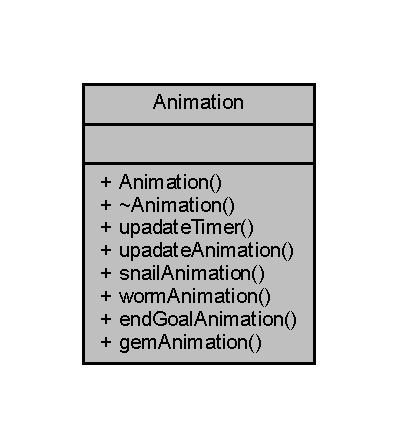
\includegraphics[width=191pt]{class_animation__coll__graph}
\end{center}
\end{figure}
\subsection*{Public Member Functions}
\begin{DoxyCompactItemize}
\item 
\hyperlink{class_animation_a3937169e447959e16931cf95ea0bea42}{Animation} (float)
\item 
\hyperlink{class_animation_a401b68793d4fbf48d481c030ee4b2a16}{$\sim$\+Animation} ()
\item 
void \hyperlink{class_animation_aa1b39bd3c7b83eea908d6e15896206ca}{upadate\+Timer} (float)
\item 
void \hyperlink{class_animation_a46ac949b21a0aed488953ee0a47ec35f}{upadate\+Animation} (char, \hyperlink{class_entity}{Entity} $\ast$)
\item 
void \hyperlink{class_animation_a64378ac8df319e785e93e8e2ff9b4f7d}{snail\+Animation} (\hyperlink{class_entity}{Entity} $\ast$)
\item 
void \hyperlink{class_animation_a28698eae748a6bcac0bbbafb1c62f32b}{worm\+Animation} (\hyperlink{class_entity}{Entity} $\ast$)
\item 
void \hyperlink{class_animation_aa991142b70b9d07bde2a2b4a934fae16}{end\+Goal\+Animation} (\hyperlink{class_entity}{Entity} $\ast$)
\item 
void \hyperlink{class_animation_a988b1ced0cf9d9a64ed3fb0891e3c563}{gem\+Animation} (int, \hyperlink{class_entity}{Entity} $\ast$)
\end{DoxyCompactItemize}


\subsection{Detailed Description}
Creates a \hyperlink{class_animation}{Animation} object to handle the animations. 

\subsection{Constructor \& Destructor Documentation}
\hypertarget{class_animation_a3937169e447959e16931cf95ea0bea42}{\index{Animation@{Animation}!Animation@{Animation}}
\index{Animation@{Animation}!Animation@{Animation}}
\subsubsection[{Animation}]{\setlength{\rightskip}{0pt plus 5cm}Animation\+::\+Animation (
\begin{DoxyParamCaption}
\item[{float}]{in\+Length}
\end{DoxyParamCaption}
)}}\label{class_animation_a3937169e447959e16931cf95ea0bea42}
Constructs an \hyperlink{class_animation}{Animation} object Constructs the \hyperlink{class_animation}{Animation} object. 
\begin{DoxyParams}{Parameters}
{\em float} & the length of the timer \\
\hline
\end{DoxyParams}
\hypertarget{class_animation_a401b68793d4fbf48d481c030ee4b2a16}{\index{Animation@{Animation}!````~Animation@{$\sim$\+Animation}}
\index{````~Animation@{$\sim$\+Animation}!Animation@{Animation}}
\subsubsection[{$\sim$\+Animation}]{\setlength{\rightskip}{0pt plus 5cm}Animation\+::$\sim$\+Animation (
\begin{DoxyParamCaption}
{}
\end{DoxyParamCaption}
)}}\label{class_animation_a401b68793d4fbf48d481c030ee4b2a16}
De-\/constructs a \hyperlink{class_animation}{Animation} object De-\/constructs the \hyperlink{class_animation}{Animation} object 

\subsection{Member Function Documentation}
\hypertarget{class_animation_aa991142b70b9d07bde2a2b4a934fae16}{\index{Animation@{Animation}!end\+Goal\+Animation@{end\+Goal\+Animation}}
\index{end\+Goal\+Animation@{end\+Goal\+Animation}!Animation@{Animation}}
\subsubsection[{end\+Goal\+Animation}]{\setlength{\rightskip}{0pt plus 5cm}void Animation\+::end\+Goal\+Animation (
\begin{DoxyParamCaption}
\item[{{\bf Entity} $\ast$}]{entity}
\end{DoxyParamCaption}
)}}\label{class_animation_aa991142b70b9d07bde2a2b4a934fae16}
Performs the animation for the end goal 
\begin{DoxyParams}{Parameters}
{\em \hyperlink{class_entity}{Entity}} & $\ast$ the entity to use the \hyperlink{class_animation}{Animation} \\
\hline
\end{DoxyParams}


Here is the call graph for this function\+:
\nopagebreak
\begin{figure}[H]
\begin{center}
\leavevmode
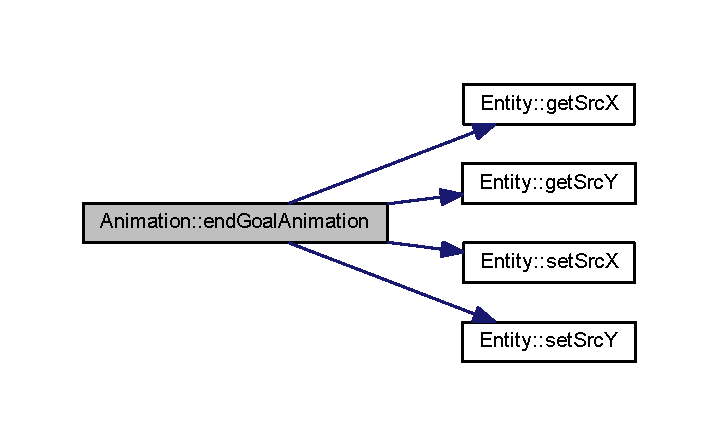
\includegraphics[width=345pt]{class_animation_aa991142b70b9d07bde2a2b4a934fae16_cgraph}
\end{center}
\end{figure}




Here is the caller graph for this function\+:
\nopagebreak
\begin{figure}[H]
\begin{center}
\leavevmode
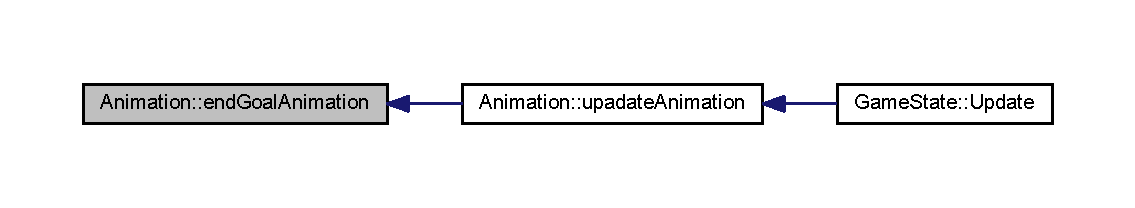
\includegraphics[width=350pt]{class_animation_aa991142b70b9d07bde2a2b4a934fae16_icgraph}
\end{center}
\end{figure}


\hypertarget{class_animation_a988b1ced0cf9d9a64ed3fb0891e3c563}{\index{Animation@{Animation}!gem\+Animation@{gem\+Animation}}
\index{gem\+Animation@{gem\+Animation}!Animation@{Animation}}
\subsubsection[{gem\+Animation}]{\setlength{\rightskip}{0pt plus 5cm}void Animation\+::gem\+Animation (
\begin{DoxyParamCaption}
\item[{int}]{type, }
\item[{{\bf Entity} $\ast$}]{entity}
\end{DoxyParamCaption}
)}}\label{class_animation_a988b1ced0cf9d9a64ed3fb0891e3c563}
Performs the timer test and animation for the \hyperlink{class_gem}{Gem} 
\begin{DoxyParams}{Parameters}
{\em int} & the type of \hyperlink{class_gem}{Gem} \\
\hline
{\em \hyperlink{class_entity}{Entity}} & $\ast$ the entity to use the \hyperlink{class_animation}{Animation} \\
\hline
\end{DoxyParams}


Here is the call graph for this function\+:
\nopagebreak
\begin{figure}[H]
\begin{center}
\leavevmode
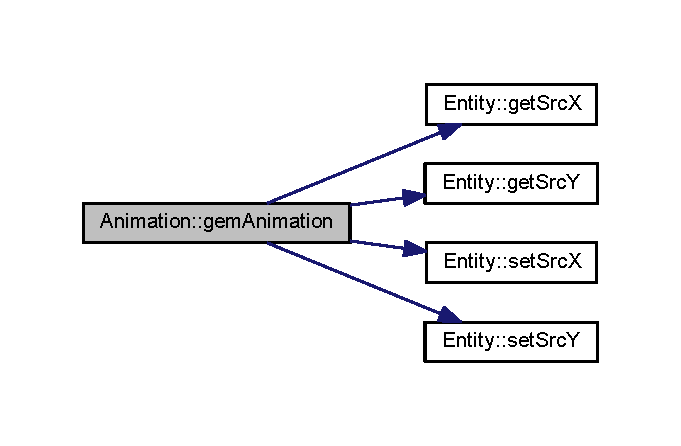
\includegraphics[width=327pt]{class_animation_a988b1ced0cf9d9a64ed3fb0891e3c563_cgraph}
\end{center}
\end{figure}




Here is the caller graph for this function\+:
\nopagebreak
\begin{figure}[H]
\begin{center}
\leavevmode
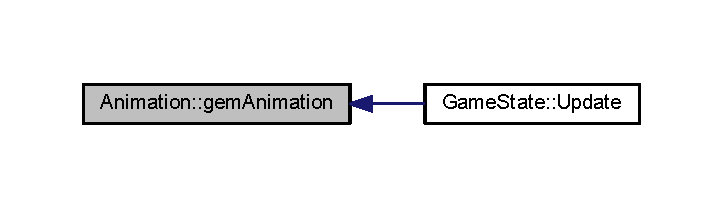
\includegraphics[width=347pt]{class_animation_a988b1ced0cf9d9a64ed3fb0891e3c563_icgraph}
\end{center}
\end{figure}


\hypertarget{class_animation_a64378ac8df319e785e93e8e2ff9b4f7d}{\index{Animation@{Animation}!snail\+Animation@{snail\+Animation}}
\index{snail\+Animation@{snail\+Animation}!Animation@{Animation}}
\subsubsection[{snail\+Animation}]{\setlength{\rightskip}{0pt plus 5cm}void Animation\+::snail\+Animation (
\begin{DoxyParamCaption}
\item[{{\bf Entity} $\ast$}]{entity}
\end{DoxyParamCaption}
)}}\label{class_animation_a64378ac8df319e785e93e8e2ff9b4f7d}
Performs the animation for the snail 
\begin{DoxyParams}{Parameters}
{\em \hyperlink{class_entity}{Entity}} & $\ast$ the entity to use the \hyperlink{class_animation}{Animation} \\
\hline
\end{DoxyParams}


Here is the call graph for this function\+:
\nopagebreak
\begin{figure}[H]
\begin{center}
\leavevmode
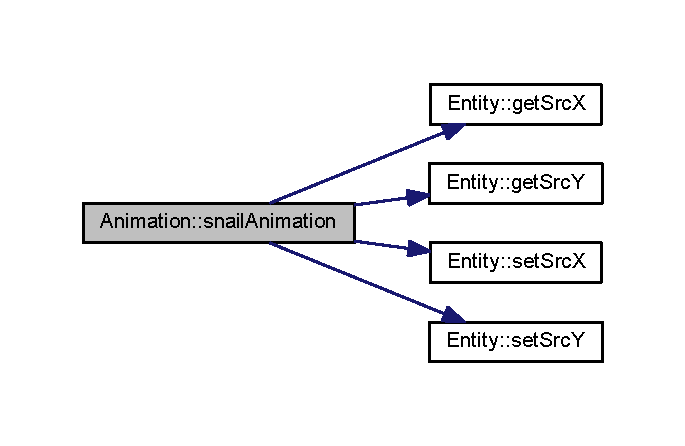
\includegraphics[width=329pt]{class_animation_a64378ac8df319e785e93e8e2ff9b4f7d_cgraph}
\end{center}
\end{figure}




Here is the caller graph for this function\+:
\nopagebreak
\begin{figure}[H]
\begin{center}
\leavevmode
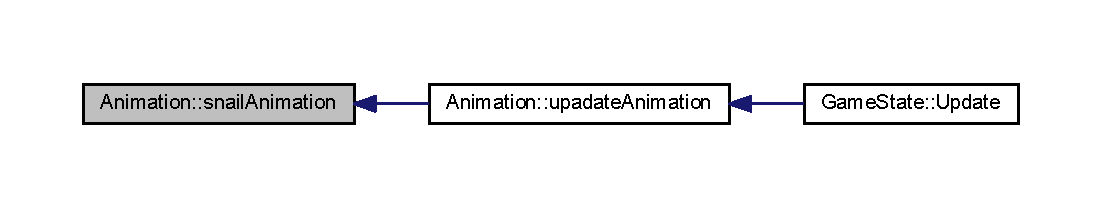
\includegraphics[width=350pt]{class_animation_a64378ac8df319e785e93e8e2ff9b4f7d_icgraph}
\end{center}
\end{figure}


\hypertarget{class_animation_a46ac949b21a0aed488953ee0a47ec35f}{\index{Animation@{Animation}!upadate\+Animation@{upadate\+Animation}}
\index{upadate\+Animation@{upadate\+Animation}!Animation@{Animation}}
\subsubsection[{upadate\+Animation}]{\setlength{\rightskip}{0pt plus 5cm}void Animation\+::upadate\+Animation (
\begin{DoxyParamCaption}
\item[{char}]{type, }
\item[{{\bf Entity} $\ast$}]{entity}
\end{DoxyParamCaption}
)}}\label{class_animation_a46ac949b21a0aed488953ee0a47ec35f}
Updates the \hyperlink{class_animation}{Animation} If the timer is 0 update the \hyperlink{class_animation}{Animation}. 
\begin{DoxyParams}{Parameters}
{\em char} & the type of the \hyperlink{class_animation}{Animation} \\
\hline
{\em \hyperlink{class_entity}{Entity}} & $\ast$ the entity to use the \hyperlink{class_animation}{Animation} \\
\hline
\end{DoxyParams}


Here is the call graph for this function\+:
\nopagebreak
\begin{figure}[H]
\begin{center}
\leavevmode
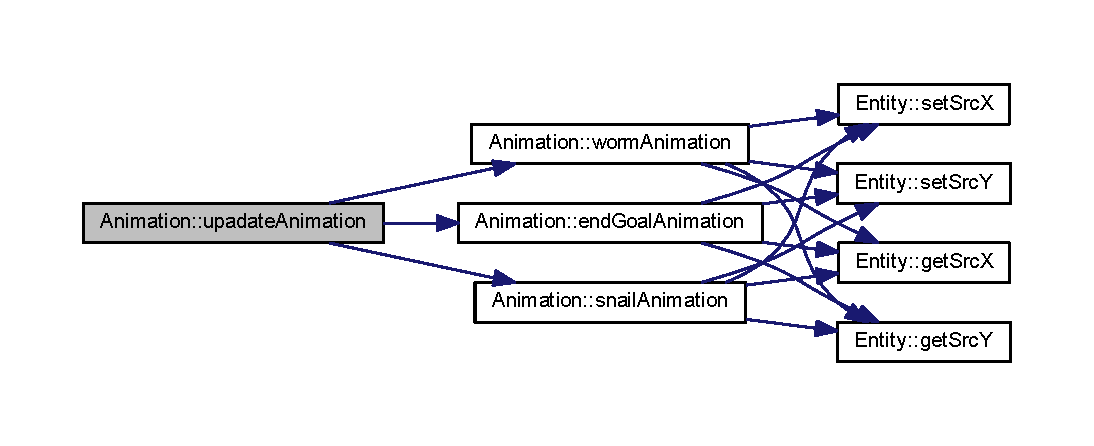
\includegraphics[width=350pt]{class_animation_a46ac949b21a0aed488953ee0a47ec35f_cgraph}
\end{center}
\end{figure}




Here is the caller graph for this function\+:
\nopagebreak
\begin{figure}[H]
\begin{center}
\leavevmode
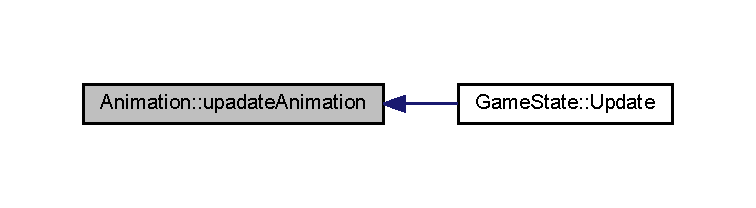
\includegraphics[width=350pt]{class_animation_a46ac949b21a0aed488953ee0a47ec35f_icgraph}
\end{center}
\end{figure}


\hypertarget{class_animation_aa1b39bd3c7b83eea908d6e15896206ca}{\index{Animation@{Animation}!upadate\+Timer@{upadate\+Timer}}
\index{upadate\+Timer@{upadate\+Timer}!Animation@{Animation}}
\subsubsection[{upadate\+Timer}]{\setlength{\rightskip}{0pt plus 5cm}void Animation\+::upadate\+Timer (
\begin{DoxyParamCaption}
\item[{float}]{delta\+Time}
\end{DoxyParamCaption}
)}}\label{class_animation_aa1b39bd3c7b83eea908d6e15896206ca}
Updates the timer Updates the timer using the delta time. If the timer is now greater than 1, then reset the timer to 0. 
\begin{DoxyParams}{Parameters}
{\em float} & the delta time \\
\hline
\end{DoxyParams}


Here is the caller graph for this function\+:
\nopagebreak
\begin{figure}[H]
\begin{center}
\leavevmode
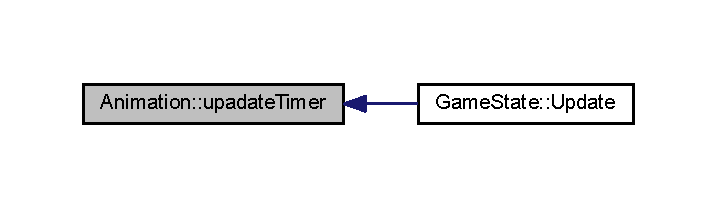
\includegraphics[width=344pt]{class_animation_aa1b39bd3c7b83eea908d6e15896206ca_icgraph}
\end{center}
\end{figure}


\hypertarget{class_animation_a28698eae748a6bcac0bbbafb1c62f32b}{\index{Animation@{Animation}!worm\+Animation@{worm\+Animation}}
\index{worm\+Animation@{worm\+Animation}!Animation@{Animation}}
\subsubsection[{worm\+Animation}]{\setlength{\rightskip}{0pt plus 5cm}void Animation\+::worm\+Animation (
\begin{DoxyParamCaption}
\item[{{\bf Entity} $\ast$}]{entity}
\end{DoxyParamCaption}
)}}\label{class_animation_a28698eae748a6bcac0bbbafb1c62f32b}
Performs the animation for the worm 
\begin{DoxyParams}{Parameters}
{\em \hyperlink{class_entity}{Entity}} & $\ast$ the entity to use the \hyperlink{class_animation}{Animation} \\
\hline
\end{DoxyParams}


Here is the call graph for this function\+:
\nopagebreak
\begin{figure}[H]
\begin{center}
\leavevmode
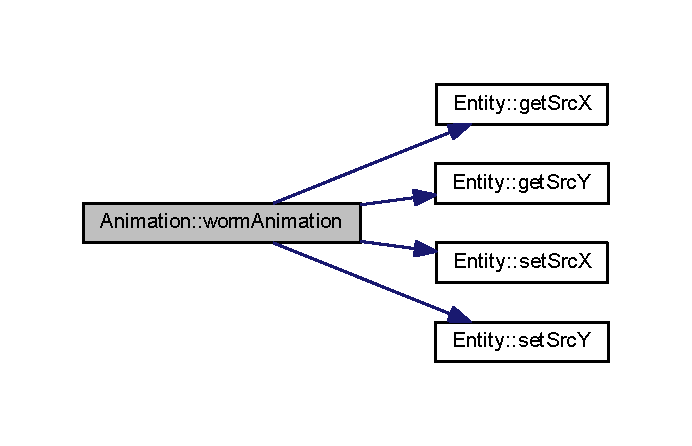
\includegraphics[width=332pt]{class_animation_a28698eae748a6bcac0bbbafb1c62f32b_cgraph}
\end{center}
\end{figure}




Here is the caller graph for this function\+:
\nopagebreak
\begin{figure}[H]
\begin{center}
\leavevmode
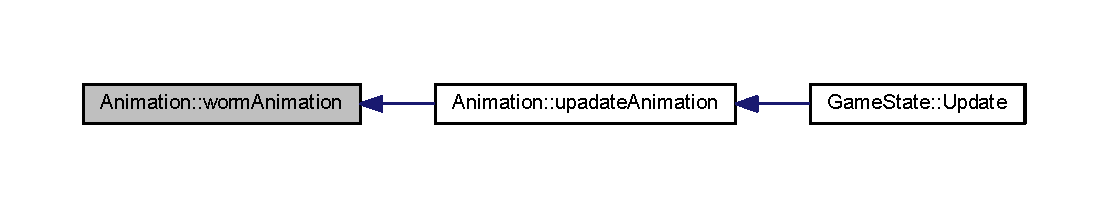
\includegraphics[width=350pt]{class_animation_a28698eae748a6bcac0bbbafb1c62f32b_icgraph}
\end{center}
\end{figure}




The documentation for this class was generated from the following files\+:\begin{DoxyCompactItemize}
\item 
P\+G\+G\+Assignment1\+S\+D\+L/animation.\+h\item 
P\+G\+G\+Assignment1\+S\+D\+L/animation.\+cpp\end{DoxyCompactItemize}

\hypertarget{class_audio}{\section{Audio Class Reference}
\label{class_audio}\index{Audio@{Audio}}
}


Creates a \hyperlink{class_audio}{Audio} object to handle the S\+D\+L\+\_\+\+Mixer. Done using help from \href{http://www.lazyfoo.net/tutorials/SDL/21_sound_effects_and_music/index.php}{\tt http\+://www.\+lazyfoo.\+net/tutorials/\+S\+D\+L/21\+\_\+sound\+\_\+effects\+\_\+and\+\_\+music/index.\+php}.  




{\ttfamily \#include $<$audio.\+h$>$}

\subsection*{Public Member Functions}
\begin{DoxyCompactItemize}
\item 
\hyperlink{class_audio_ae1900ee0e5254fe0c96e0b423ea02777}{Audio} (std\+::string, bool)
\item 
\hyperlink{class_audio_ae8f54deecb5f48511aaab469e80294d6}{$\sim$\+Audio} ()
\item 
void \hyperlink{class_audio_a15f1ea89039f6dbbb2260bb34f9dabdd}{start\+Audio} ()
\item 
void \hyperlink{class_audio_aea41cc6feaed4b1ab5957ea499509f55}{play\+Effect} ()
\item 
void \hyperlink{class_audio_a5d73ae24c80b37df5f167016de9c9296}{stop\+Audio} ()
\end{DoxyCompactItemize}


\subsection{Detailed Description}
Creates a \hyperlink{class_audio}{Audio} object to handle the S\+D\+L\+\_\+\+Mixer. Done using help from \href{http://www.lazyfoo.net/tutorials/SDL/21_sound_effects_and_music/index.php}{\tt http\+://www.\+lazyfoo.\+net/tutorials/\+S\+D\+L/21\+\_\+sound\+\_\+effects\+\_\+and\+\_\+music/index.\+php}. 

\subsection{Constructor \& Destructor Documentation}
\hypertarget{class_audio_ae1900ee0e5254fe0c96e0b423ea02777}{\index{Audio@{Audio}!Audio@{Audio}}
\index{Audio@{Audio}!Audio@{Audio}}
\subsubsection[{Audio}]{\setlength{\rightskip}{0pt plus 5cm}Audio\+::\+Audio (
\begin{DoxyParamCaption}
\item[{std\+::string}]{file, }
\item[{bool}]{music}
\end{DoxyParamCaption}
)}}\label{class_audio_ae1900ee0e5254fe0c96e0b423ea02777}
Constructs an \hyperlink{class_audio}{Audio} object Constructs the \hyperlink{class_audio}{Audio} object. 
\begin{DoxyParams}{Parameters}
{\em std\+::string} & the file to be loaded \\
\hline
{\em bool} & is it a music file? if false its a sound file \\
\hline
\end{DoxyParams}
\hypertarget{class_audio_ae8f54deecb5f48511aaab469e80294d6}{\index{Audio@{Audio}!````~Audio@{$\sim$\+Audio}}
\index{````~Audio@{$\sim$\+Audio}!Audio@{Audio}}
\subsubsection[{$\sim$\+Audio}]{\setlength{\rightskip}{0pt plus 5cm}Audio\+::$\sim$\+Audio (
\begin{DoxyParamCaption}
{}
\end{DoxyParamCaption}
)}}\label{class_audio_ae8f54deecb5f48511aaab469e80294d6}
De-\/constructs a \hyperlink{class_audio}{Audio} object De-\/constructs the \hyperlink{class_audio}{Audio} object 

\subsection{Member Function Documentation}
\hypertarget{class_audio_aea41cc6feaed4b1ab5957ea499509f55}{\index{Audio@{Audio}!play\+Effect@{play\+Effect}}
\index{play\+Effect@{play\+Effect}!Audio@{Audio}}
\subsubsection[{play\+Effect}]{\setlength{\rightskip}{0pt plus 5cm}void Audio\+::play\+Effect (
\begin{DoxyParamCaption}
{}
\end{DoxyParamCaption}
)}}\label{class_audio_aea41cc6feaed4b1ab5957ea499509f55}
Plays the sound Plays the sound effect \hypertarget{class_audio_a15f1ea89039f6dbbb2260bb34f9dabdd}{\index{Audio@{Audio}!start\+Audio@{start\+Audio}}
\index{start\+Audio@{start\+Audio}!Audio@{Audio}}
\subsubsection[{start\+Audio}]{\setlength{\rightskip}{0pt plus 5cm}void Audio\+::start\+Audio (
\begin{DoxyParamCaption}
{}
\end{DoxyParamCaption}
)}}\label{class_audio_a15f1ea89039f6dbbb2260bb34f9dabdd}
Starts the \hyperlink{class_audio}{Audio} playing Starts the \hyperlink{class_audio}{Audio} playing, also checks if not playing and starts again \hypertarget{class_audio_a5d73ae24c80b37df5f167016de9c9296}{\index{Audio@{Audio}!stop\+Audio@{stop\+Audio}}
\index{stop\+Audio@{stop\+Audio}!Audio@{Audio}}
\subsubsection[{stop\+Audio}]{\setlength{\rightskip}{0pt plus 5cm}void Audio\+::stop\+Audio (
\begin{DoxyParamCaption}
{}
\end{DoxyParamCaption}
)}}\label{class_audio_a5d73ae24c80b37df5f167016de9c9296}
Stops the \hyperlink{class_audio}{Audio} playing 

The documentation for this class was generated from the following files\+:\begin{DoxyCompactItemize}
\item 
P\+G\+G\+Assignment1\+S\+D\+L/audio.\+h\item 
P\+G\+G\+Assignment1\+S\+D\+L/audio.\+cpp\end{DoxyCompactItemize}

\hypertarget{class_background}{\section{Background Class Reference}
\label{class_background}\index{Background@{Background}}
}


Creates a \hyperlink{class_background}{Background} object that inherits \hyperlink{class_entity}{Entity}. Creates a \hyperlink{class_background}{Background} object with a velocity, and position check. It also has a \hyperlink{class_texture}{Texture} (including variables for the source and destination dimensions), position and velocity in entity.  




{\ttfamily \#include $<$background.\+h$>$}

Inheritance diagram for Background\+:\begin{figure}[H]
\begin{center}
\leavevmode
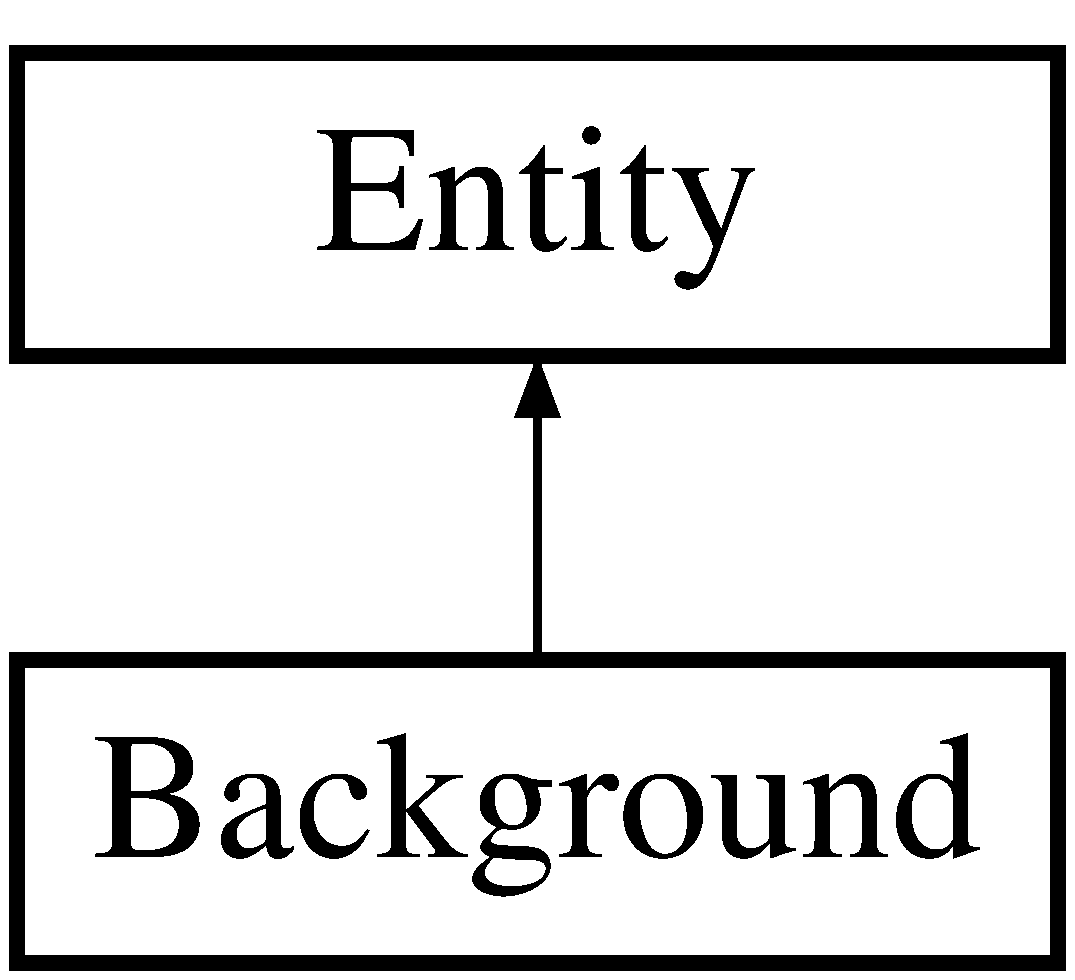
\includegraphics[height=2.000000cm]{class_background}
\end{center}
\end{figure}
\subsection*{Public Member Functions}
\begin{DoxyCompactItemize}
\item 
\hyperlink{class_background_a31d67c19cf5dd14c0f07b91e89c8b1f8}{Background} (\hyperlink{class_texture}{Texture} $\ast$, int)
\item 
\hyperlink{class_background_a36754df1deb720393217ade59da41557}{$\sim$\+Background} ()
\item 
void \hyperlink{class_background_a9b358e049be63be31b9241410288514f}{set\+Velocity} (float)
\item 
void \hyperlink{class_background_a1cb5afc5d8857ec4db6c6d393375a4c2}{update\+X} (float)
\item 
int \hyperlink{class_background_a25e0286050106340c34d91d3f1d0f4df}{get\+Type} ()
\item 
bool \hyperlink{class_background_a5f3e6259bb294391cf39d776456e7748}{get\+Moveable} ()
\item 
bool \hyperlink{class_background_a9e2c4dc2434c8123c1fabceecb53a7c0}{get\+Right\+Moveable} ()
\item 
bool \hyperlink{class_background_a6b49b6e383fed26938af98773f0952fa}{get\+Left\+Moveable} ()
\end{DoxyCompactItemize}
\subsection*{Additional Inherited Members}


\subsection{Detailed Description}
Creates a \hyperlink{class_background}{Background} object that inherits \hyperlink{class_entity}{Entity}. Creates a \hyperlink{class_background}{Background} object with a velocity, and position check. It also has a \hyperlink{class_texture}{Texture} (including variables for the source and destination dimensions), position and velocity in entity. 

\subsection{Constructor \& Destructor Documentation}
\hypertarget{class_background_a31d67c19cf5dd14c0f07b91e89c8b1f8}{\index{Background@{Background}!Background@{Background}}
\index{Background@{Background}!Background@{Background}}
\subsubsection[{Background}]{\setlength{\rightskip}{0pt plus 5cm}Background\+::\+Background (
\begin{DoxyParamCaption}
\item[{{\bf Texture} $\ast$}]{input\+Texture, }
\item[{int}]{input\+Background\+Type}
\end{DoxyParamCaption}
)}}\label{class_background_a31d67c19cf5dd14c0f07b91e89c8b1f8}
Constructs a \hyperlink{class_background}{Background} object Constructs a \hyperlink{class_background}{Background} object using the input \hyperlink{class_texture}{Texture} and background type. All of the other variables are automatically initialized to defaults. 
\begin{DoxyParams}{Parameters}
{\em Texture$\ast$} & a pointer to a \hyperlink{class_texture}{Texture} loaded into memory. \\
\hline
{\em int} & an number between 0 an 2 that sets which of the 3 backgrounds is loaded from the texture. \\
\hline
\end{DoxyParams}
\hypertarget{class_background_a36754df1deb720393217ade59da41557}{\index{Background@{Background}!````~Background@{$\sim$\+Background}}
\index{````~Background@{$\sim$\+Background}!Background@{Background}}
\subsubsection[{$\sim$\+Background}]{\setlength{\rightskip}{0pt plus 5cm}Background\+::$\sim$\+Background (
\begin{DoxyParamCaption}
{}
\end{DoxyParamCaption}
)}}\label{class_background_a36754df1deb720393217ade59da41557}
De-\/constructs a \hyperlink{class_background}{Background} object De-\/constructs the \hyperlink{class_background}{Background} object 

\subsection{Member Function Documentation}
\hypertarget{class_background_a6b49b6e383fed26938af98773f0952fa}{\index{Background@{Background}!get\+Left\+Moveable@{get\+Left\+Moveable}}
\index{get\+Left\+Moveable@{get\+Left\+Moveable}!Background@{Background}}
\subsubsection[{get\+Left\+Moveable}]{\setlength{\rightskip}{0pt plus 5cm}bool Background\+::get\+Left\+Moveable (
\begin{DoxyParamCaption}
{}
\end{DoxyParamCaption}
)}}\label{class_background_a6b49b6e383fed26938af98773f0952fa}
Getter \# moveable left \begin{DoxyReturn}{Returns}
bool if the \hyperlink{class_background}{Background} can move left. 
\end{DoxyReturn}
\hypertarget{class_background_a5f3e6259bb294391cf39d776456e7748}{\index{Background@{Background}!get\+Moveable@{get\+Moveable}}
\index{get\+Moveable@{get\+Moveable}!Background@{Background}}
\subsubsection[{get\+Moveable}]{\setlength{\rightskip}{0pt plus 5cm}bool Background\+::get\+Moveable (
\begin{DoxyParamCaption}
{}
\end{DoxyParamCaption}
)}}\label{class_background_a5f3e6259bb294391cf39d776456e7748}
Getter \# moveable \begin{DoxyReturn}{Returns}
bool if the \hyperlink{class_background}{Background} can move. 
\end{DoxyReturn}
\hypertarget{class_background_a9e2c4dc2434c8123c1fabceecb53a7c0}{\index{Background@{Background}!get\+Right\+Moveable@{get\+Right\+Moveable}}
\index{get\+Right\+Moveable@{get\+Right\+Moveable}!Background@{Background}}
\subsubsection[{get\+Right\+Moveable}]{\setlength{\rightskip}{0pt plus 5cm}bool Background\+::get\+Right\+Moveable (
\begin{DoxyParamCaption}
{}
\end{DoxyParamCaption}
)}}\label{class_background_a9e2c4dc2434c8123c1fabceecb53a7c0}
Getter \# moveable right \begin{DoxyReturn}{Returns}
bool if the \hyperlink{class_background}{Background} can move right. 
\end{DoxyReturn}
\hypertarget{class_background_a25e0286050106340c34d91d3f1d0f4df}{\index{Background@{Background}!get\+Type@{get\+Type}}
\index{get\+Type@{get\+Type}!Background@{Background}}
\subsubsection[{get\+Type}]{\setlength{\rightskip}{0pt plus 5cm}int Background\+::get\+Type (
\begin{DoxyParamCaption}
{}
\end{DoxyParamCaption}
)}}\label{class_background_a25e0286050106340c34d91d3f1d0f4df}
Getter \# background\+Type \begin{DoxyReturn}{Returns}
int the type of the \hyperlink{class_background}{Background}. 
\end{DoxyReturn}
\hypertarget{class_background_a9b358e049be63be31b9241410288514f}{\index{Background@{Background}!set\+Velocity@{set\+Velocity}}
\index{set\+Velocity@{set\+Velocity}!Background@{Background}}
\subsubsection[{set\+Velocity}]{\setlength{\rightskip}{0pt plus 5cm}void Background\+::set\+Velocity (
\begin{DoxyParamCaption}
\item[{float}]{input\+Velocity}
\end{DoxyParamCaption}
)}}\label{class_background_a9b358e049be63be31b9241410288514f}
Setter \# velocity Sets the velocity of the \hyperlink{class_background}{Background} to the inputed velocity. 
\begin{DoxyParams}{Parameters}
{\em float} & the inputed velocity \\
\hline
\end{DoxyParams}
\hypertarget{class_background_a1cb5afc5d8857ec4db6c6d393375a4c2}{\index{Background@{Background}!update\+X@{update\+X}}
\index{update\+X@{update\+X}!Background@{Background}}
\subsubsection[{update\+X}]{\setlength{\rightskip}{0pt plus 5cm}void Background\+::update\+X (
\begin{DoxyParamCaption}
\item[{float}]{dt}
\end{DoxyParamCaption}
)}}\label{class_background_a1cb5afc5d8857ec4db6c6d393375a4c2}
Updates the x position of the \hyperlink{class_background}{Background} Performers a check on the updated position of the x to see if it within boundaries. If it is within boundaries then it updates the x position using the velocity and the inputed delta\+Time. If it is not within boundaries then it resets the x position to the boundaries. 
\begin{DoxyParams}{Parameters}
{\em float} & the inputed delta\+Time \\
\hline
\end{DoxyParams}


The documentation for this class was generated from the following files\+:\begin{DoxyCompactItemize}
\item 
P\+G\+G\+Assignment1\+S\+D\+L/background.\+h\item 
P\+G\+G\+Assignment1\+S\+D\+L/background.\+cpp\end{DoxyCompactItemize}

\hypertarget{class_block}{\section{Block Class Reference}
\label{class_block}\index{Block@{Block}}
}


Creates a \hyperlink{class_block}{Block} object that inherits \hyperlink{class_map_object}{Map\+Object}.  




{\ttfamily \#include $<$block.\+h$>$}

Inheritance diagram for Block\+:\begin{figure}[H]
\begin{center}
\leavevmode
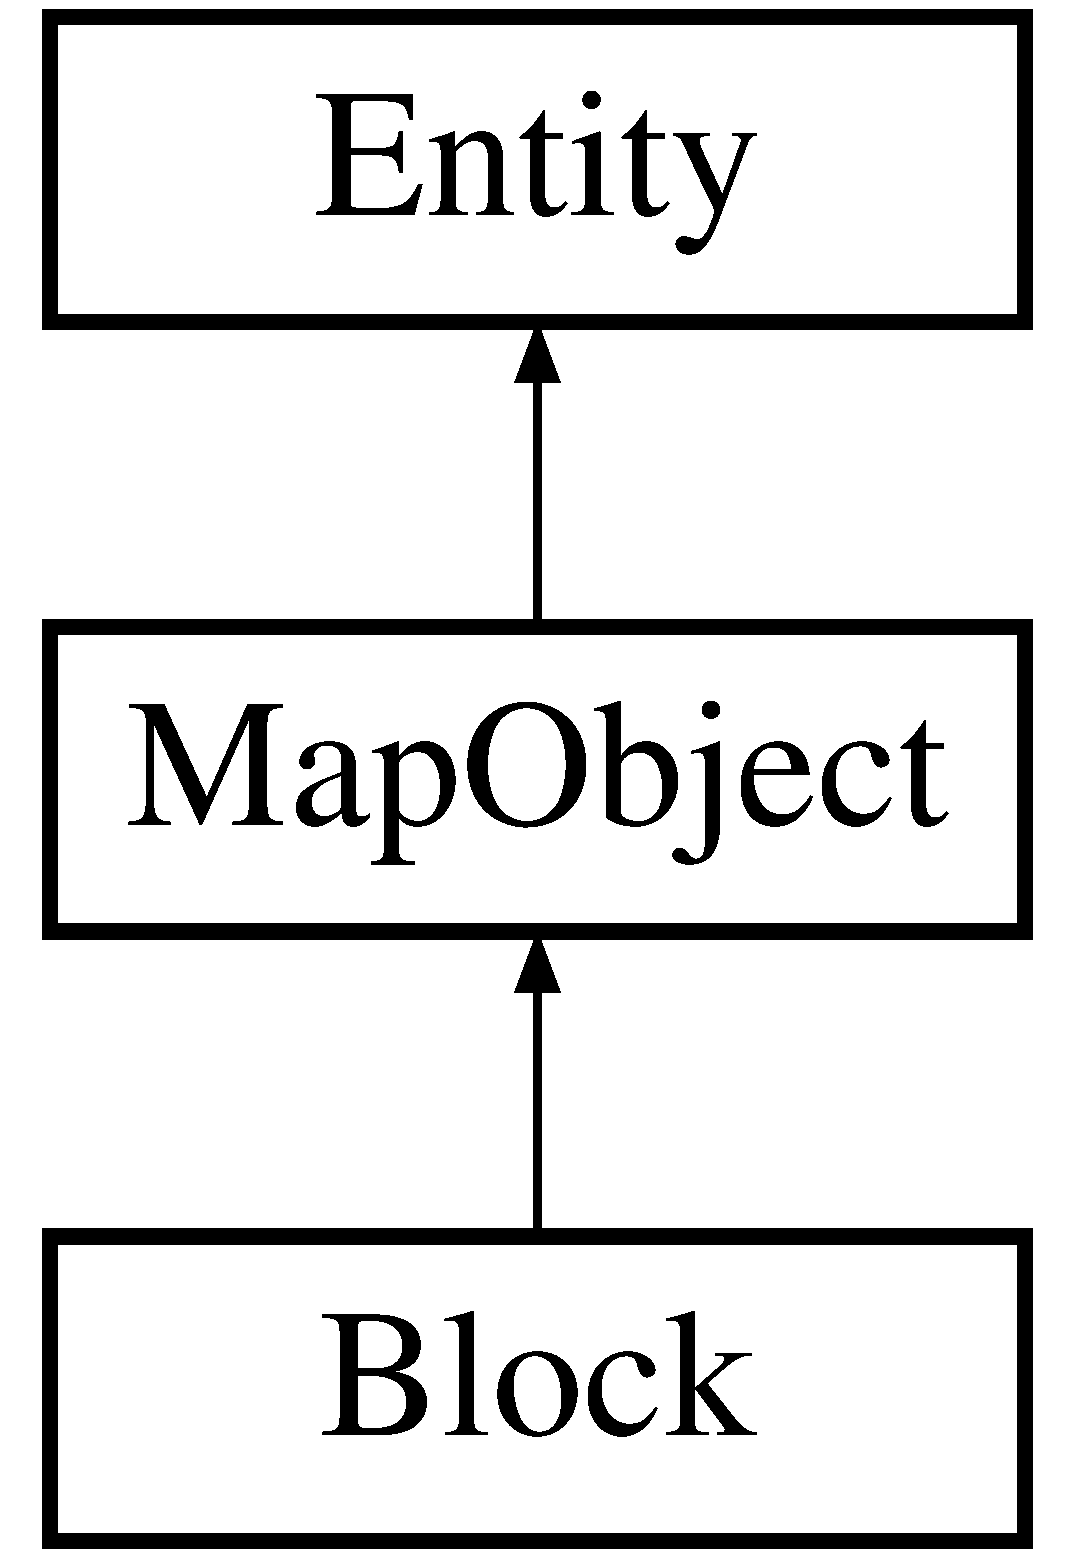
\includegraphics[height=3.000000cm]{class_block}
\end{center}
\end{figure}
\subsection*{Public Member Functions}
\begin{DoxyCompactItemize}
\item 
\hyperlink{class_block_ae82bbded382f61248fe4ab7f198f66f7}{Block} (\hyperlink{class_texture}{Texture} $\ast$, float, float, int, int, int)
\item 
\hyperlink{class_block_a19d1bd0e1cef6a865ed2745a2e648405}{$\sim$\+Block} ()
\end{DoxyCompactItemize}
\subsection*{Additional Inherited Members}


\subsection{Detailed Description}
Creates a \hyperlink{class_block}{Block} object that inherits \hyperlink{class_map_object}{Map\+Object}. 

\subsection{Constructor \& Destructor Documentation}
\hypertarget{class_block_ae82bbded382f61248fe4ab7f198f66f7}{\index{Block@{Block}!Block@{Block}}
\index{Block@{Block}!Block@{Block}}
\subsubsection[{Block}]{\setlength{\rightskip}{0pt plus 5cm}Block\+::\+Block (
\begin{DoxyParamCaption}
\item[{{\bf Texture} $\ast$}]{input\+Texture, }
\item[{float}]{input\+X, }
\item[{float}]{input\+Y, }
\item[{int}]{sprite\+Sheet\+Number\+X, }
\item[{int}]{sprite\+Sheet\+Number\+Y, }
\item[{int}]{in\+Type}
\end{DoxyParamCaption}
)}}\label{class_block_ae82bbded382f61248fe4ab7f198f66f7}
Constructs a \hyperlink{class_block}{Block} object Constructs the \hyperlink{class_block}{Block} object. 
\begin{DoxyParams}{Parameters}
{\em Texture$\ast$} & a pointer to a \hyperlink{class_texture}{Texture} loaded into memory. \\
\hline
{\em float} & initial x position. \\
\hline
{\em float} & initial y position. \\
\hline
{\em int} & the sprite sheet x number. \\
\hline
{\em int} & the sprite sheet y number. \\
\hline
{\em int} & the \hyperlink{class_block}{Block} type. \\
\hline
\end{DoxyParams}
\hypertarget{class_block_a19d1bd0e1cef6a865ed2745a2e648405}{\index{Block@{Block}!````~Block@{$\sim$\+Block}}
\index{````~Block@{$\sim$\+Block}!Block@{Block}}
\subsubsection[{$\sim$\+Block}]{\setlength{\rightskip}{0pt plus 5cm}Block\+::$\sim$\+Block (
\begin{DoxyParamCaption}
{}
\end{DoxyParamCaption}
)}}\label{class_block_a19d1bd0e1cef6a865ed2745a2e648405}
De-\/constructs a \hyperlink{class_block}{Block} object De-\/constructs the \hyperlink{class_block}{Block} object 

The documentation for this class was generated from the following files\+:\begin{DoxyCompactItemize}
\item 
P\+G\+G\+Assignment1\+S\+D\+L/block.\+h\item 
P\+G\+G\+Assignment1\+S\+D\+L/block.\+cpp\end{DoxyCompactItemize}

\hypertarget{class_collision}{\section{Collision Class Reference}
\label{class_collision}\index{Collision@{Collision}}
}


Creates an \hyperlink{class_collision}{Collision} object. The \hyperlink{class_collision}{Collision} object is for use with detecting \hyperlink{class_collision}{Collision}. Used help from \href{http://higherorderfun.com/blog/2012/05/20/the-guide-to-implementing-2d-platformers/}{\tt http\+://higherorderfun.\+com/blog/2012/05/20/the-\/guide-\/to-\/implementing-\/2d-\/platformers/} in the type 2 section.  




{\ttfamily \#include $<$collision.\+h$>$}

\subsection*{Public Member Functions}
\begin{DoxyCompactItemize}
\item 
\hyperlink{class_collision_a975df63cb6f3b4d746191ff8348598fb}{Collision} (\hyperlink{class_player}{Player} $\ast$, \hyperlink{class_map_loader}{Map\+Loader} $\ast$)
\item 
\hyperlink{class_collision_a19ae49bcb3b16f4622443a34a171590c}{$\sim$\+Collision} ()
\item 
void \hyperlink{class_collision_ac7635cf9b887dcd4ffc3cf15f35e39a9}{player\+Collision\+Test} (float)
\item 
void \hyperlink{class_collision_a8a7c7bbaa789c0867559d79ef186dd84}{gem\+Action} (int)
\item 
void \hyperlink{class_collision_aaf2c586cbf92070483282ab66090e5dc}{block\+Action} (int)
\end{DoxyCompactItemize}


\subsection{Detailed Description}
Creates an \hyperlink{class_collision}{Collision} object. The \hyperlink{class_collision}{Collision} object is for use with detecting \hyperlink{class_collision}{Collision}. Used help from \href{http://higherorderfun.com/blog/2012/05/20/the-guide-to-implementing-2d-platformers/}{\tt http\+://higherorderfun.\+com/blog/2012/05/20/the-\/guide-\/to-\/implementing-\/2d-\/platformers/} in the type 2 section. 

\subsection{Constructor \& Destructor Documentation}
\hypertarget{class_collision_a975df63cb6f3b4d746191ff8348598fb}{\index{Collision@{Collision}!Collision@{Collision}}
\index{Collision@{Collision}!Collision@{Collision}}
\subsubsection[{Collision}]{\setlength{\rightskip}{0pt plus 5cm}Collision\+::\+Collision (
\begin{DoxyParamCaption}
\item[{{\bf Player} $\ast$}]{input\+Player, }
\item[{{\bf Map\+Loader} $\ast$}]{input\+Map}
\end{DoxyParamCaption}
)}}\label{class_collision_a975df63cb6f3b4d746191ff8348598fb}
Constructs an \hyperlink{class_collision}{Collision} object Constructs the \hyperlink{class_collision}{Collision} object. 
\begin{DoxyParams}{Parameters}
{\em \hyperlink{class_player}{Player}} & $\ast$ pointer to the \hyperlink{class_player}{Player} \\
\hline
{\em \hyperlink{class_map_loader}{Map\+Loader}} & $\ast$ pointer to the \hyperlink{class_map_loader}{Map\+Loader} \\
\hline
\end{DoxyParams}
\hypertarget{class_collision_a19ae49bcb3b16f4622443a34a171590c}{\index{Collision@{Collision}!````~Collision@{$\sim$\+Collision}}
\index{````~Collision@{$\sim$\+Collision}!Collision@{Collision}}
\subsubsection[{$\sim$\+Collision}]{\setlength{\rightskip}{0pt plus 5cm}Collision\+::$\sim$\+Collision (
\begin{DoxyParamCaption}
{}
\end{DoxyParamCaption}
)}}\label{class_collision_a19ae49bcb3b16f4622443a34a171590c}
De-\/constructs an \hyperlink{class_collision}{Collision} object De-\/constructs the \hyperlink{class_collision}{Collision} object 

\subsection{Member Function Documentation}
\hypertarget{class_collision_aaf2c586cbf92070483282ab66090e5dc}{\index{Collision@{Collision}!block\+Action@{block\+Action}}
\index{block\+Action@{block\+Action}!Collision@{Collision}}
\subsubsection[{block\+Action}]{\setlength{\rightskip}{0pt plus 5cm}void Collision\+::block\+Action (
\begin{DoxyParamCaption}
\item[{int}]{i}
\end{DoxyParamCaption}
)}}\label{class_collision_aaf2c586cbf92070483282ab66090e5dc}
\hyperlink{class_block}{Block} collision action Performs the action that happens when the player collides with a \hyperlink{class_block}{Block} 
\begin{DoxyParams}{Parameters}
{\em int} & the index of the \hyperlink{class_block}{Block} that has been collided with \\
\hline
\end{DoxyParams}
\hypertarget{class_collision_a8a7c7bbaa789c0867559d79ef186dd84}{\index{Collision@{Collision}!gem\+Action@{gem\+Action}}
\index{gem\+Action@{gem\+Action}!Collision@{Collision}}
\subsubsection[{gem\+Action}]{\setlength{\rightskip}{0pt plus 5cm}void Collision\+::gem\+Action (
\begin{DoxyParamCaption}
\item[{int}]{i}
\end{DoxyParamCaption}
)}}\label{class_collision_a8a7c7bbaa789c0867559d79ef186dd84}
\hyperlink{class_gem}{Gem} collision action Performs the action that happens when the player collides with a \hyperlink{class_gem}{Gem} 
\begin{DoxyParams}{Parameters}
{\em int} & the index of the \hyperlink{class_gem}{Gem} that has been collided with \\
\hline
\end{DoxyParams}
\hypertarget{class_collision_ac7635cf9b887dcd4ffc3cf15f35e39a9}{\index{Collision@{Collision}!player\+Collision\+Test@{player\+Collision\+Test}}
\index{player\+Collision\+Test@{player\+Collision\+Test}!Collision@{Collision}}
\subsubsection[{player\+Collision\+Test}]{\setlength{\rightskip}{0pt plus 5cm}void Collision\+::player\+Collision\+Test (
\begin{DoxyParamCaption}
\item[{float}]{delta\+Time}
\end{DoxyParamCaption}
)}}\label{class_collision_ac7635cf9b887dcd4ffc3cf15f35e39a9}
\hyperlink{class_player}{Player} collision test Tests if the \hyperlink{class_player}{Player} collides with an object. 
\begin{DoxyParams}{Parameters}
{\em float} & the delta time \\
\hline
\end{DoxyParams}


The documentation for this class was generated from the following files\+:\begin{DoxyCompactItemize}
\item 
P\+G\+G\+Assignment1\+S\+D\+L/collision.\+h\item 
P\+G\+G\+Assignment1\+S\+D\+L/collision.\+cpp\end{DoxyCompactItemize}

\hypertarget{class_creature}{\section{Creature Class Reference}
\label{class_creature}\index{Creature@{Creature}}
}


Creates a \hyperlink{class_creature}{Creature} object that inherits \hyperlink{class_entity}{Entity}.  




{\ttfamily \#include $<$creature.\+h$>$}

Inheritance diagram for Creature\+:\begin{figure}[H]
\begin{center}
\leavevmode
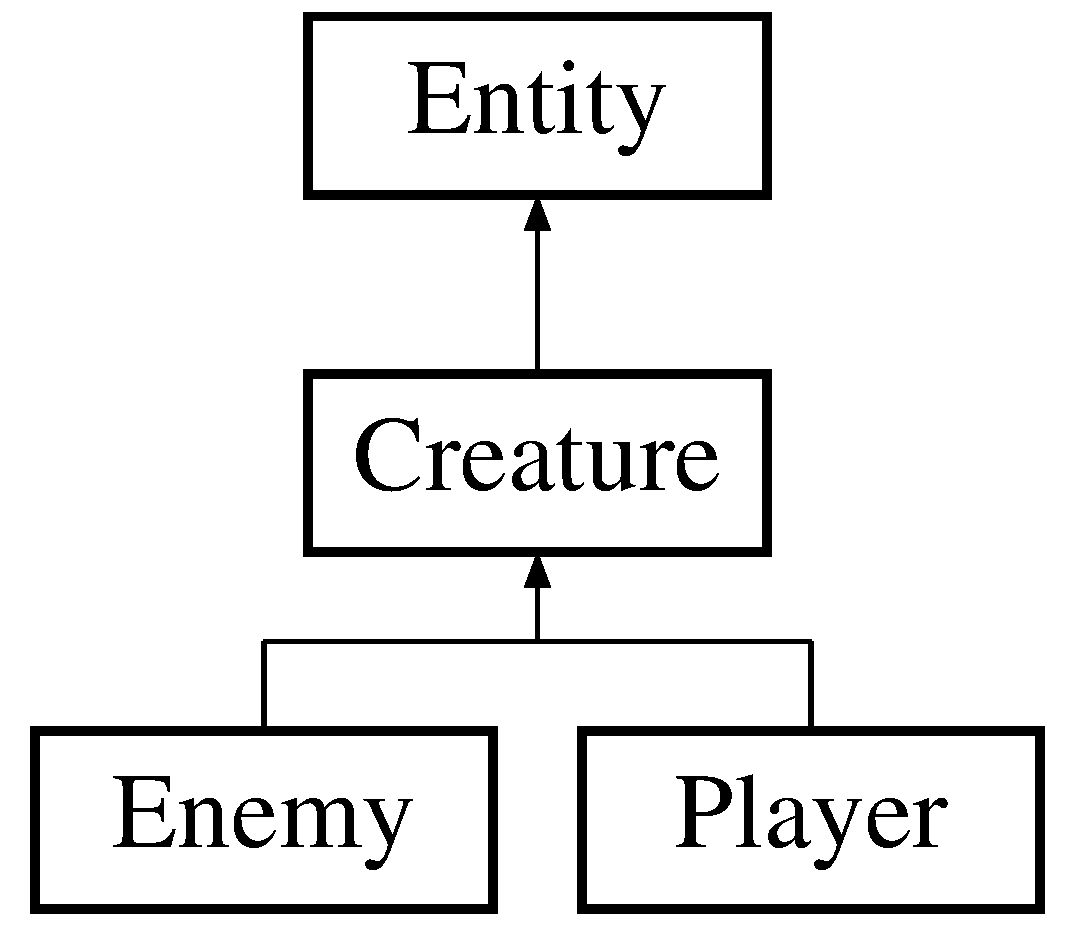
\includegraphics[height=3.000000cm]{class_creature}
\end{center}
\end{figure}
\subsection*{Public Member Functions}
\begin{DoxyCompactItemize}
\item 
\hyperlink{class_creature_a597cc3b08ee17de46c3e7ec3cf0d9b58}{Creature} ()
\item 
\hyperlink{class_creature_aa991b23f4813fbdb6f875204ed49814d}{$\sim$\+Creature} ()
\item 
void \hyperlink{class_creature_ab2ad7544f3c7fd24829c8c28ea5c667f}{set\+Velocity\+X} (float)
\item 
void \hyperlink{class_creature_a5aa971df9bf484d62fbe6413f01a661b}{set\+Velocity\+Y} (float)
\item 
void \hyperlink{class_creature_ac10e36c59bd7ec83708b46235aefbc33}{update\+X} (float)
\item 
void \hyperlink{class_creature_ab2bdf6ddfe183c828761bae1da81be47}{update\+Y} (float)
\item 
float \hyperlink{class_creature_a405b16c27bc5617e9c37ac01e166c785}{get\+Velocity\+X} ()
\item 
float \hyperlink{class_creature_a0ca2c7cccf8c8182dcad7a3b6737380b}{get\+Velocity\+Y} ()
\end{DoxyCompactItemize}
\subsection*{Protected Attributes}
\begin{DoxyCompactItemize}
\item 
\hypertarget{class_creature_a6e857406fb17f893ebace230ff8aa05f}{float {\bfseries velocity\+X}}\label{class_creature_a6e857406fb17f893ebace230ff8aa05f}

\item 
\hypertarget{class_creature_a8a3cb01fd7b9d05372749fc9e04ab8dd}{float {\bfseries velocity\+Y}}\label{class_creature_a8a3cb01fd7b9d05372749fc9e04ab8dd}

\end{DoxyCompactItemize}


\subsection{Detailed Description}
Creates a \hyperlink{class_creature}{Creature} object that inherits \hyperlink{class_entity}{Entity}. 

\subsection{Constructor \& Destructor Documentation}
\hypertarget{class_creature_a597cc3b08ee17de46c3e7ec3cf0d9b58}{\index{Creature@{Creature}!Creature@{Creature}}
\index{Creature@{Creature}!Creature@{Creature}}
\subsubsection[{Creature}]{\setlength{\rightskip}{0pt plus 5cm}Creature\+::\+Creature (
\begin{DoxyParamCaption}
{}
\end{DoxyParamCaption}
)}}\label{class_creature_a597cc3b08ee17de46c3e7ec3cf0d9b58}
Constructs \hyperlink{class_creature}{Creature} object Constructs a \hyperlink{class_creature}{Creature} object. \hypertarget{class_creature_aa991b23f4813fbdb6f875204ed49814d}{\index{Creature@{Creature}!````~Creature@{$\sim$\+Creature}}
\index{````~Creature@{$\sim$\+Creature}!Creature@{Creature}}
\subsubsection[{$\sim$\+Creature}]{\setlength{\rightskip}{0pt plus 5cm}Creature\+::$\sim$\+Creature (
\begin{DoxyParamCaption}
{}
\end{DoxyParamCaption}
)}}\label{class_creature_aa991b23f4813fbdb6f875204ed49814d}
De-\/constructs a \hyperlink{class_creature}{Creature} object De-\/constructs the \hyperlink{class_creature}{Creature} object 

\subsection{Member Function Documentation}
\hypertarget{class_creature_a405b16c27bc5617e9c37ac01e166c785}{\index{Creature@{Creature}!get\+Velocity\+X@{get\+Velocity\+X}}
\index{get\+Velocity\+X@{get\+Velocity\+X}!Creature@{Creature}}
\subsubsection[{get\+Velocity\+X}]{\setlength{\rightskip}{0pt plus 5cm}float Creature\+::get\+Velocity\+X (
\begin{DoxyParamCaption}
{}
\end{DoxyParamCaption}
)}}\label{class_creature_a405b16c27bc5617e9c37ac01e166c785}
Getter \# x velocity \begin{DoxyReturn}{Returns}
the x velocity of the \hyperlink{class_creature}{Creature} object. 
\end{DoxyReturn}
\hypertarget{class_creature_a0ca2c7cccf8c8182dcad7a3b6737380b}{\index{Creature@{Creature}!get\+Velocity\+Y@{get\+Velocity\+Y}}
\index{get\+Velocity\+Y@{get\+Velocity\+Y}!Creature@{Creature}}
\subsubsection[{get\+Velocity\+Y}]{\setlength{\rightskip}{0pt plus 5cm}float Creature\+::get\+Velocity\+Y (
\begin{DoxyParamCaption}
{}
\end{DoxyParamCaption}
)}}\label{class_creature_a0ca2c7cccf8c8182dcad7a3b6737380b}
Getter \# y velocity \begin{DoxyReturn}{Returns}
the y velocity of the \hyperlink{class_creature}{Creature} object. 
\end{DoxyReturn}
\hypertarget{class_creature_ab2ad7544f3c7fd24829c8c28ea5c667f}{\index{Creature@{Creature}!set\+Velocity\+X@{set\+Velocity\+X}}
\index{set\+Velocity\+X@{set\+Velocity\+X}!Creature@{Creature}}
\subsubsection[{set\+Velocity\+X}]{\setlength{\rightskip}{0pt plus 5cm}void Creature\+::set\+Velocity\+X (
\begin{DoxyParamCaption}
\item[{float}]{input\+Velocity}
\end{DoxyParamCaption}
)}}\label{class_creature_ab2ad7544f3c7fd24829c8c28ea5c667f}
Setter \# x velocity Sets the x velocity of the \hyperlink{class_creature}{Creature} object to the inputed velocity. 
\begin{DoxyParams}{Parameters}
{\em float} & the inputed velocity \\
\hline
\end{DoxyParams}
\hypertarget{class_creature_a5aa971df9bf484d62fbe6413f01a661b}{\index{Creature@{Creature}!set\+Velocity\+Y@{set\+Velocity\+Y}}
\index{set\+Velocity\+Y@{set\+Velocity\+Y}!Creature@{Creature}}
\subsubsection[{set\+Velocity\+Y}]{\setlength{\rightskip}{0pt plus 5cm}void Creature\+::set\+Velocity\+Y (
\begin{DoxyParamCaption}
\item[{float}]{input\+Velocity}
\end{DoxyParamCaption}
)}}\label{class_creature_a5aa971df9bf484d62fbe6413f01a661b}
Setter \# y velocity Sets the y velocity of the \hyperlink{class_creature}{Creature} object to the inputed velocity. 
\begin{DoxyParams}{Parameters}
{\em float} & the inputed velocity \\
\hline
\end{DoxyParams}
\hypertarget{class_creature_ac10e36c59bd7ec83708b46235aefbc33}{\index{Creature@{Creature}!update\+X@{update\+X}}
\index{update\+X@{update\+X}!Creature@{Creature}}
\subsubsection[{update\+X}]{\setlength{\rightskip}{0pt plus 5cm}void Creature\+::update\+X (
\begin{DoxyParamCaption}
\item[{float}]{dt}
\end{DoxyParamCaption}
)}}\label{class_creature_ac10e36c59bd7ec83708b46235aefbc33}
Updates the x position of the \hyperlink{class_creature}{Creature} 
\begin{DoxyParams}{Parameters}
{\em float} & the inputed delta\+Time \\
\hline
\end{DoxyParams}
\hypertarget{class_creature_ab2bdf6ddfe183c828761bae1da81be47}{\index{Creature@{Creature}!update\+Y@{update\+Y}}
\index{update\+Y@{update\+Y}!Creature@{Creature}}
\subsubsection[{update\+Y}]{\setlength{\rightskip}{0pt plus 5cm}void Creature\+::update\+Y (
\begin{DoxyParamCaption}
\item[{float}]{dt}
\end{DoxyParamCaption}
)}}\label{class_creature_ab2bdf6ddfe183c828761bae1da81be47}
Updates the y position of the \hyperlink{class_creature}{Creature} 
\begin{DoxyParams}{Parameters}
{\em float} & the inputed delta\+Time \\
\hline
\end{DoxyParams}


The documentation for this class was generated from the following files\+:\begin{DoxyCompactItemize}
\item 
P\+G\+G\+Assignment1\+S\+D\+L/creature.\+h\item 
P\+G\+G\+Assignment1\+S\+D\+L/creature.\+cpp\end{DoxyCompactItemize}

\hypertarget{class_credits_state}{\section{Credits\+State Class Reference}
\label{class_credits_state}\index{Credits\+State@{Credits\+State}}
}


Creates a \hyperlink{class_credits_state}{Credits\+State} object. Creates a \hyperlink{class_credits_state}{Credits\+State} object that inherits \hyperlink{class_state}{State}.  




{\ttfamily \#include $<$credits\+State.\+h$>$}

Inheritance diagram for Credits\+State\+:\begin{figure}[H]
\begin{center}
\leavevmode
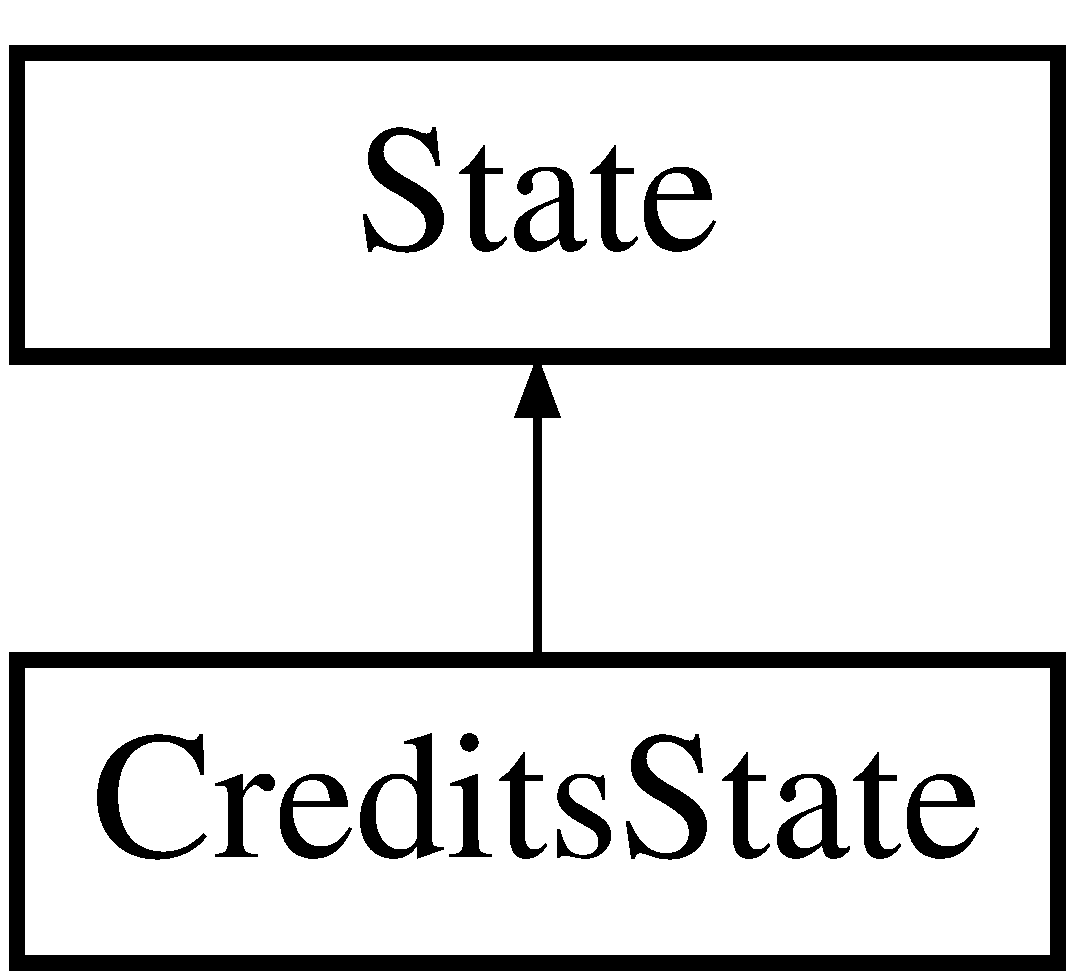
\includegraphics[height=2.000000cm]{class_credits_state}
\end{center}
\end{figure}
\subsection*{Public Member Functions}
\begin{DoxyCompactItemize}
\item 
\hyperlink{class_credits_state_a0904712a229318e1b8e43d1c6bb27b7c}{Credits\+State} (\hyperlink{class_state_manager}{State\+Manager} $\ast$, S\+D\+L\+\_\+\+Renderer $\ast$)
\item 
\hyperlink{class_credits_state_abf1cbbd68bbbbf05eae5ab4721f2233a}{$\sim$\+Credits\+State} ()
\item 
bool \hyperlink{class_credits_state_a952d9a50d529f1ba4d883b4a37f558d4}{Handle\+S\+D\+L\+Events} ()
\item 
void \hyperlink{class_credits_state_ab9ad90f4b1c6ddab6ff1234a92c9aec1}{Update} (float delta\+Time)
\item 
void \hyperlink{class_credits_state_a4027aad0c48b505a74faef47470622a1}{Draw} ()
\end{DoxyCompactItemize}
\subsection*{Additional Inherited Members}


\subsection{Detailed Description}
Creates a \hyperlink{class_credits_state}{Credits\+State} object. Creates a \hyperlink{class_credits_state}{Credits\+State} object that inherits \hyperlink{class_state}{State}. 

\subsection{Constructor \& Destructor Documentation}
\hypertarget{class_credits_state_a0904712a229318e1b8e43d1c6bb27b7c}{\index{Credits\+State@{Credits\+State}!Credits\+State@{Credits\+State}}
\index{Credits\+State@{Credits\+State}!Credits\+State@{Credits\+State}}
\subsubsection[{Credits\+State}]{\setlength{\rightskip}{0pt plus 5cm}Credits\+State\+::\+Credits\+State (
\begin{DoxyParamCaption}
\item[{{\bf State\+Manager} $\ast$}]{in\+State\+Manager, }
\item[{S\+D\+L\+\_\+\+Renderer $\ast$}]{in\+Renderer}
\end{DoxyParamCaption}
)}}\label{class_credits_state_a0904712a229318e1b8e43d1c6bb27b7c}
Constructs a \hyperlink{class_credits_state}{Credits\+State} object Constructs a \hyperlink{class_credits_state}{Credits\+State} object 
\begin{DoxyParams}{Parameters}
{\em \hyperlink{class_state_manager}{State\+Manager}} & $\ast$ a pointer to the \hyperlink{class_state_manager}{State\+Manager} \\
\hline
{\em S\+D\+L\+\_\+\+Renderer} & $\ast$ a pointer to the renderer in use. \\
\hline
\end{DoxyParams}
\hypertarget{class_credits_state_abf1cbbd68bbbbf05eae5ab4721f2233a}{\index{Credits\+State@{Credits\+State}!````~Credits\+State@{$\sim$\+Credits\+State}}
\index{````~Credits\+State@{$\sim$\+Credits\+State}!Credits\+State@{Credits\+State}}
\subsubsection[{$\sim$\+Credits\+State}]{\setlength{\rightskip}{0pt plus 5cm}Credits\+State\+::$\sim$\+Credits\+State (
\begin{DoxyParamCaption}
{}
\end{DoxyParamCaption}
)}}\label{class_credits_state_abf1cbbd68bbbbf05eae5ab4721f2233a}
De-\/constructs a \hyperlink{class_credits_state}{Credits\+State} object De-\/constructs the \hyperlink{class_credits_state}{Credits\+State} object 

\subsection{Member Function Documentation}
\hypertarget{class_credits_state_a4027aad0c48b505a74faef47470622a1}{\index{Credits\+State@{Credits\+State}!Draw@{Draw}}
\index{Draw@{Draw}!Credits\+State@{Credits\+State}}
\subsubsection[{Draw}]{\setlength{\rightskip}{0pt plus 5cm}void Credits\+State\+::\+Draw (
\begin{DoxyParamCaption}
{}
\end{DoxyParamCaption}
)\hspace{0.3cm}{\ttfamily [virtual]}}}\label{class_credits_state_a4027aad0c48b505a74faef47470622a1}
A function to draw to the screen A function to draw to the screen using the renderer 

Implements \hyperlink{class_state_a8b0cdb0e7450a9bb3580a33dfbe4d981}{State}.

\hypertarget{class_credits_state_a952d9a50d529f1ba4d883b4a37f558d4}{\index{Credits\+State@{Credits\+State}!Handle\+S\+D\+L\+Events@{Handle\+S\+D\+L\+Events}}
\index{Handle\+S\+D\+L\+Events@{Handle\+S\+D\+L\+Events}!Credits\+State@{Credits\+State}}
\subsubsection[{Handle\+S\+D\+L\+Events}]{\setlength{\rightskip}{0pt plus 5cm}bool Credits\+State\+::\+Handle\+S\+D\+L\+Events (
\begin{DoxyParamCaption}
{}
\end{DoxyParamCaption}
)\hspace{0.3cm}{\ttfamily [virtual]}}}\label{class_credits_state_a952d9a50d529f1ba4d883b4a37f558d4}
A function to handle the S\+D\+L events A function to handle the S\+D\+L events for use with the \hyperlink{class_credits_state}{Credits\+State} \begin{DoxyReturn}{Returns}
bool if false then quit \hyperlink{class_credits_state}{Credits\+State} 
\end{DoxyReturn}


Implements \hyperlink{class_state_a648d9182cab9aeb914ef778f94e2b437}{State}.

\hypertarget{class_credits_state_ab9ad90f4b1c6ddab6ff1234a92c9aec1}{\index{Credits\+State@{Credits\+State}!Update@{Update}}
\index{Update@{Update}!Credits\+State@{Credits\+State}}
\subsubsection[{Update}]{\setlength{\rightskip}{0pt plus 5cm}void Credits\+State\+::\+Update (
\begin{DoxyParamCaption}
\item[{float}]{delta\+Time}
\end{DoxyParamCaption}
)\hspace{0.3cm}{\ttfamily [virtual]}}}\label{class_credits_state_ab9ad90f4b1c6ddab6ff1234a92c9aec1}
A function to update the \hyperlink{class_credits_state}{Credits\+State} A function to update the \hyperlink{class_credits_state}{Credits\+State} to allow the \hyperlink{class_credits_state}{Credits\+State} to run 
\begin{DoxyParams}{Parameters}
{\em float} & the delta time \\
\hline
\end{DoxyParams}


Implements \hyperlink{class_state_a770f40188fdfc64bc95a5166fef12e02}{State}.



The documentation for this class was generated from the following files\+:\begin{DoxyCompactItemize}
\item 
P\+G\+G\+Assignment1\+S\+D\+L/credits\+State.\+h\item 
P\+G\+G\+Assignment1\+S\+D\+L/credits\+State.\+cpp\end{DoxyCompactItemize}

\hypertarget{class_enemy}{\section{Enemy Class Reference}
\label{class_enemy}\index{Enemy@{Enemy}}
}


Creates an \hyperlink{class_enemy}{Enemy} object that inherits \hyperlink{class_creature}{Creature} which in turn inherits \hyperlink{class_entity}{Entity}.  




{\ttfamily \#include $<$enemy.\+h$>$}

Inheritance diagram for Enemy\+:\begin{figure}[H]
\begin{center}
\leavevmode
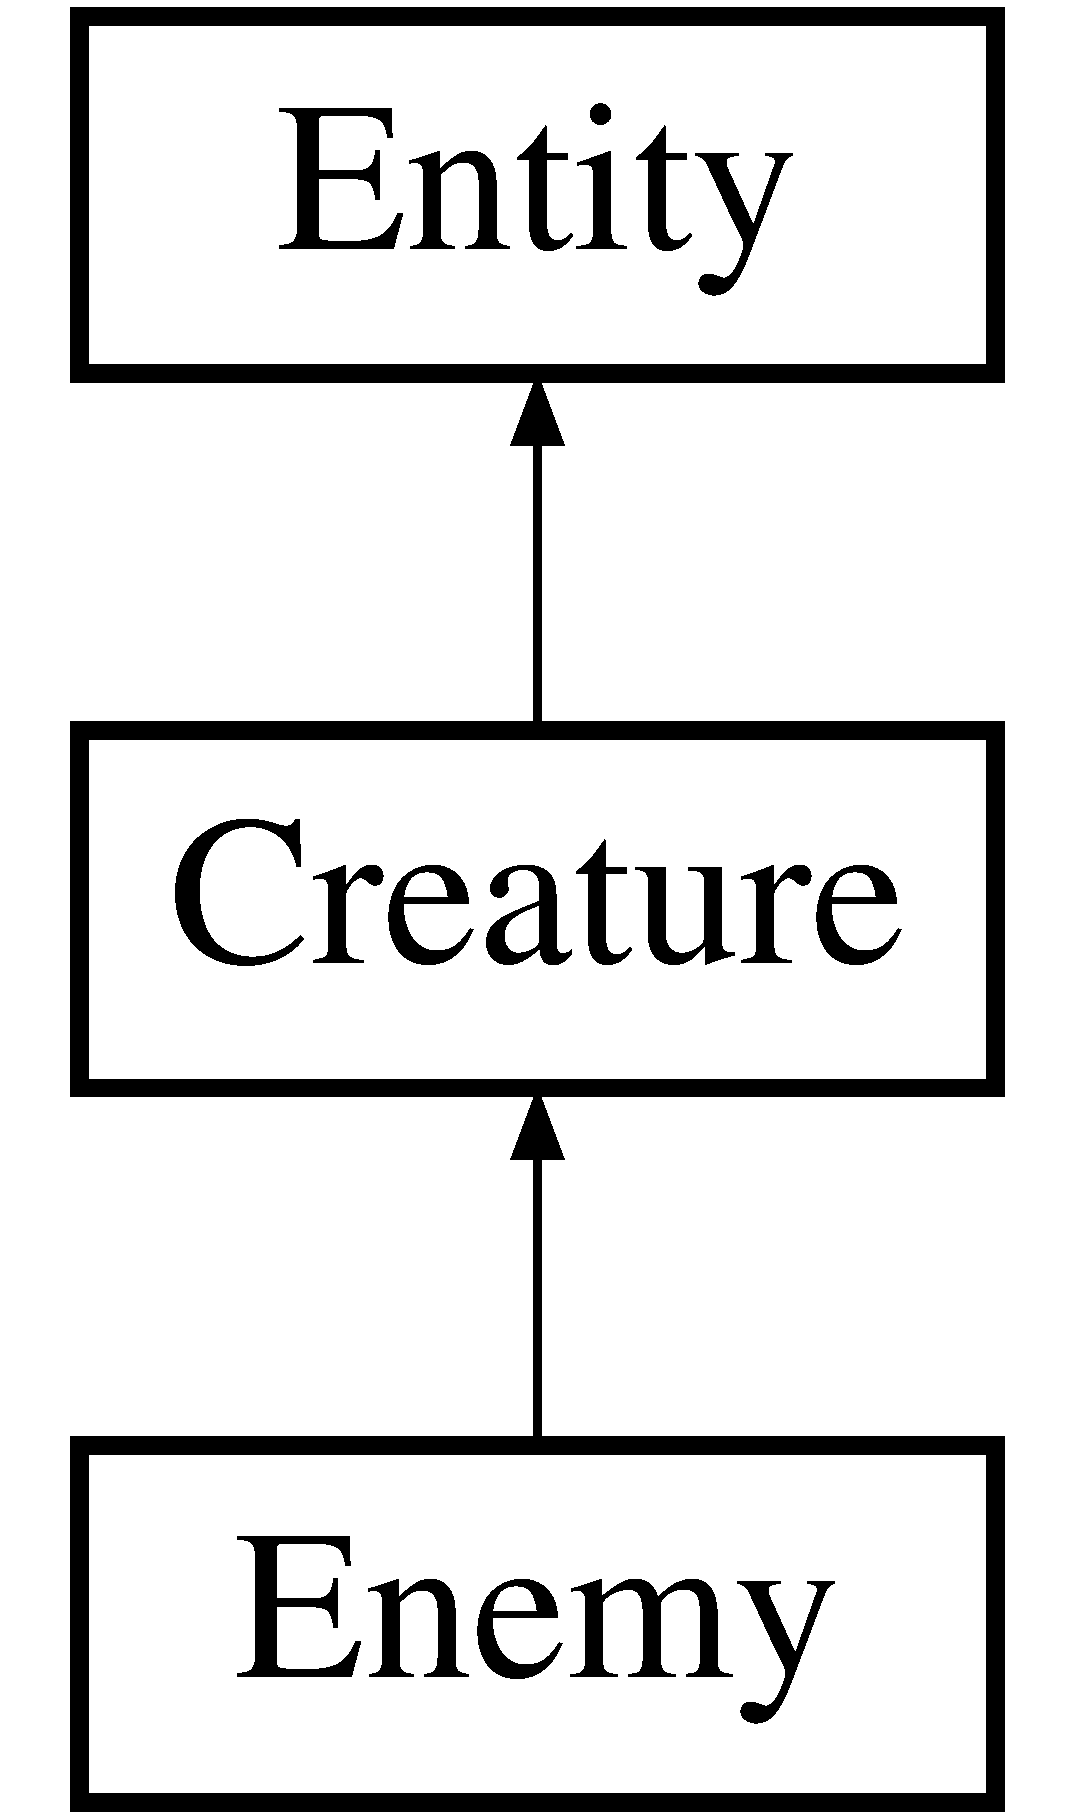
\includegraphics[height=3.000000cm]{class_enemy}
\end{center}
\end{figure}
\subsection*{Public Member Functions}
\begin{DoxyCompactItemize}
\item 
\hyperlink{class_enemy_a94f30d348b6d2840fd71675472ba38dd}{Enemy} ()
\item 
\hyperlink{class_enemy_ac0eec4755e28c02688065f9657150ac3}{$\sim$\+Enemy} ()
\end{DoxyCompactItemize}
\subsection*{Additional Inherited Members}


\subsection{Detailed Description}
Creates an \hyperlink{class_enemy}{Enemy} object that inherits \hyperlink{class_creature}{Creature} which in turn inherits \hyperlink{class_entity}{Entity}. 

\subsection{Constructor \& Destructor Documentation}
\hypertarget{class_enemy_a94f30d348b6d2840fd71675472ba38dd}{\index{Enemy@{Enemy}!Enemy@{Enemy}}
\index{Enemy@{Enemy}!Enemy@{Enemy}}
\subsubsection[{Enemy}]{\setlength{\rightskip}{0pt plus 5cm}Enemy\+::\+Enemy (
\begin{DoxyParamCaption}
{}
\end{DoxyParamCaption}
)}}\label{class_enemy_a94f30d348b6d2840fd71675472ba38dd}
Constructs an \hyperlink{class_enemy}{Enemy} object Constructs the \hyperlink{class_enemy}{Enemy} object. \hypertarget{class_enemy_ac0eec4755e28c02688065f9657150ac3}{\index{Enemy@{Enemy}!````~Enemy@{$\sim$\+Enemy}}
\index{````~Enemy@{$\sim$\+Enemy}!Enemy@{Enemy}}
\subsubsection[{$\sim$\+Enemy}]{\setlength{\rightskip}{0pt plus 5cm}Enemy\+::$\sim$\+Enemy (
\begin{DoxyParamCaption}
{}
\end{DoxyParamCaption}
)}}\label{class_enemy_ac0eec4755e28c02688065f9657150ac3}
De-\/constructs an \hyperlink{class_enemy}{Enemy} object De-\/constructs the \hyperlink{class_enemy}{Enemy} object 

The documentation for this class was generated from the following files\+:\begin{DoxyCompactItemize}
\item 
P\+G\+G\+Assignment1\+S\+D\+L/enemy.\+h\item 
P\+G\+G\+Assignment1\+S\+D\+L/enemy.\+cpp\end{DoxyCompactItemize}

\hypertarget{class_entity}{\section{Entity Class Reference}
\label{class_entity}\index{Entity@{Entity}}
}


Creates an \hyperlink{class_entity}{Entity} object Creates an \hyperlink{class_entity}{Entity} object with a \hyperlink{class_texture}{Texture} (including variables for the source and destination dimensions) and position.  




{\ttfamily \#include $<$entity.\+h$>$}

Inheritance diagram for Entity\+:\begin{figure}[H]
\begin{center}
\leavevmode
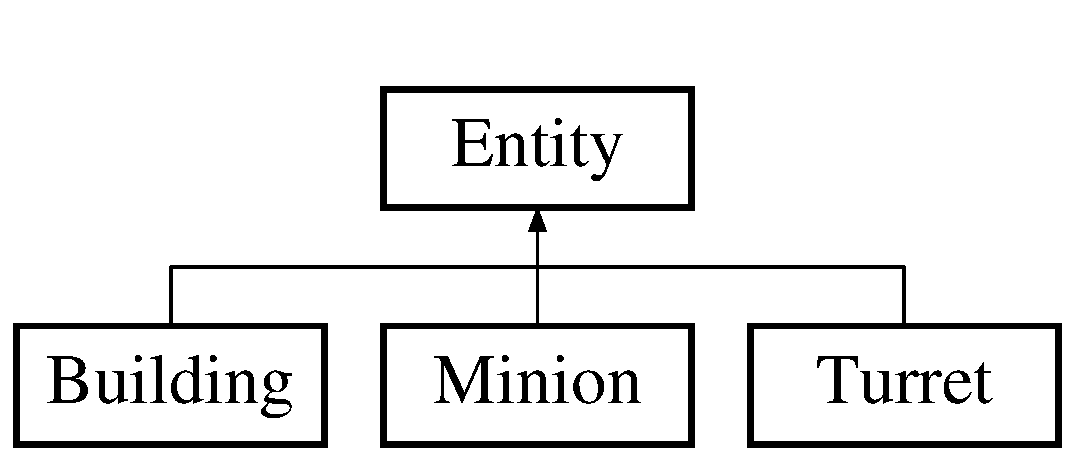
\includegraphics[height=2.000000cm]{class_entity}
\end{center}
\end{figure}
\subsection*{Public Member Functions}
\begin{DoxyCompactItemize}
\item 
\hyperlink{class_entity_a980f368aa07ce358583982821533a54a}{Entity} ()
\item 
\hyperlink{class_entity_adf6d3f7cb1b2ba029b6b048a395cc8ae}{$\sim$\+Entity} ()
\item 
void \hyperlink{class_entity_a2224871711ac97a54af338ddefc25ac9}{display} (S\+D\+L\+\_\+\+Renderer $\ast$)
\item 
void \hyperlink{class_entity_a38e2f110d39426ba4823296b4294dd74}{set\+X} (float)
\item 
void \hyperlink{class_entity_a8896110a266bdec69b14d34ec6374df8}{set\+Y} (float)
\item 
float \hyperlink{class_entity_abc5b6d26c039bf3bf6faa766990768b4}{get\+X} ()
\item 
float \hyperlink{class_entity_ab6dd7b404c13754202acfe3d2c65c77b}{get\+Y} ()
\item 
void \hyperlink{class_entity_a0c4ef1c69d6054cebf71445d98bb3afc}{set\+Health} (int)
\item 
int \hyperlink{class_entity_a2b0140ae8c77c0e3654b070ee3c7fe57}{get\+Health} ()
\item 
void \hyperlink{class_entity_a008de3cd38f0a2d2533c3384e54569cc}{set\+Cost} (int)
\item 
int \hyperlink{class_entity_a57cbd6215579c3181414c352a920ba10}{get\+Cost} ()
\end{DoxyCompactItemize}
\subsection*{Protected Attributes}
\begin{DoxyCompactItemize}
\item 
\hypertarget{class_entity_a94c6b2b4a46ea4885b5fa5859d7d68e7}{\hyperlink{class_texture}{Texture} $\ast$ {\bfseries texture}}\label{class_entity_a94c6b2b4a46ea4885b5fa5859d7d68e7}

\item 
\hypertarget{class_entity_a8a44ea56b660b9ac701d32931a066dce}{int {\bfseries src\+Width}}\label{class_entity_a8a44ea56b660b9ac701d32931a066dce}

\item 
\hypertarget{class_entity_a98172dbf203df1a9a7279a5e005eae08}{int {\bfseries src\+Height}}\label{class_entity_a98172dbf203df1a9a7279a5e005eae08}

\item 
\hypertarget{class_entity_a2871ef137e228ba7d431d5c65abcfd5c}{int {\bfseries src\+X}}\label{class_entity_a2871ef137e228ba7d431d5c65abcfd5c}

\item 
\hypertarget{class_entity_a24a5a921e7adf221357a6afd5ce5ec75}{int {\bfseries src\+Y}}\label{class_entity_a24a5a921e7adf221357a6afd5ce5ec75}

\item 
\hypertarget{class_entity_a58bf3e06b7431307e26c4adccae8cf11}{int {\bfseries width}}\label{class_entity_a58bf3e06b7431307e26c4adccae8cf11}

\item 
\hypertarget{class_entity_a5591f1e3ea630c4d8063038728587ab8}{int {\bfseries height}}\label{class_entity_a5591f1e3ea630c4d8063038728587ab8}

\item 
\hypertarget{class_entity_abc2d19ee6ff26b8520428894da6a8f68}{float {\bfseries x}}\label{class_entity_abc2d19ee6ff26b8520428894da6a8f68}

\item 
\hypertarget{class_entity_af4966f81d91cc8f8d5eb9e9002240c49}{float {\bfseries y}}\label{class_entity_af4966f81d91cc8f8d5eb9e9002240c49}

\item 
\hypertarget{class_entity_ab5bf0c97620636e04b271601e2133884}{int {\bfseries health}}\label{class_entity_ab5bf0c97620636e04b271601e2133884}

\item 
\hypertarget{class_entity_af0d86b6186484391164c2572c4a1be64}{int {\bfseries cost}}\label{class_entity_af0d86b6186484391164c2572c4a1be64}

\end{DoxyCompactItemize}


\subsection{Detailed Description}
Creates an \hyperlink{class_entity}{Entity} object Creates an \hyperlink{class_entity}{Entity} object with a \hyperlink{class_texture}{Texture} (including variables for the source and destination dimensions) and position. 

\subsection{Constructor \& Destructor Documentation}
\hypertarget{class_entity_a980f368aa07ce358583982821533a54a}{\index{Entity@{Entity}!Entity@{Entity}}
\index{Entity@{Entity}!Entity@{Entity}}
\subsubsection[{Entity}]{\setlength{\rightskip}{0pt plus 5cm}Entity\+::\+Entity (
\begin{DoxyParamCaption}
{}
\end{DoxyParamCaption}
)}}\label{class_entity_a980f368aa07ce358583982821533a54a}
Constructs an \hyperlink{class_entity}{Entity} object Constructs the \hyperlink{class_entity}{Entity} object \hypertarget{class_entity_adf6d3f7cb1b2ba029b6b048a395cc8ae}{\index{Entity@{Entity}!````~Entity@{$\sim$\+Entity}}
\index{````~Entity@{$\sim$\+Entity}!Entity@{Entity}}
\subsubsection[{$\sim$\+Entity}]{\setlength{\rightskip}{0pt plus 5cm}Entity\+::$\sim$\+Entity (
\begin{DoxyParamCaption}
{}
\end{DoxyParamCaption}
)}}\label{class_entity_adf6d3f7cb1b2ba029b6b048a395cc8ae}
De-\/constructs an \hyperlink{class_entity}{Entity} object De-\/constructs the \hyperlink{class_entity}{Entity} object 

\subsection{Member Function Documentation}
\hypertarget{class_entity_a2224871711ac97a54af338ddefc25ac9}{\index{Entity@{Entity}!display@{display}}
\index{display@{display}!Entity@{Entity}}
\subsubsection[{display}]{\setlength{\rightskip}{0pt plus 5cm}void Entity\+::display (
\begin{DoxyParamCaption}
\item[{S\+D\+L\+\_\+\+Renderer $\ast$}]{renderer}
\end{DoxyParamCaption}
)}}\label{class_entity_a2224871711ac97a54af338ddefc25ac9}
Displays the modified \hyperlink{class_texture}{Texture} renderer Pushes the texture to the renderer using the dimensions specified in the \hyperlink{class_entity}{Entity}. 
\begin{DoxyParams}{Parameters}
{\em S\+D\+L\+\_\+\+Renderer$\ast$} & The renderer. \\
\hline
\end{DoxyParams}
\hypertarget{class_entity_a57cbd6215579c3181414c352a920ba10}{\index{Entity@{Entity}!get\+Cost@{get\+Cost}}
\index{get\+Cost@{get\+Cost}!Entity@{Entity}}
\subsubsection[{get\+Cost}]{\setlength{\rightskip}{0pt plus 5cm}int Entity\+::get\+Cost (
\begin{DoxyParamCaption}
{}
\end{DoxyParamCaption}
)}}\label{class_entity_a57cbd6215579c3181414c352a920ba10}
Getter \# cost Returns the cost of the \hyperlink{class_entity}{Entity} object. \hypertarget{class_entity_a2b0140ae8c77c0e3654b070ee3c7fe57}{\index{Entity@{Entity}!get\+Health@{get\+Health}}
\index{get\+Health@{get\+Health}!Entity@{Entity}}
\subsubsection[{get\+Health}]{\setlength{\rightskip}{0pt plus 5cm}int Entity\+::get\+Health (
\begin{DoxyParamCaption}
{}
\end{DoxyParamCaption}
)}}\label{class_entity_a2b0140ae8c77c0e3654b070ee3c7fe57}
Getter \# health Returns the health of the \hyperlink{class_entity}{Entity} object. \hypertarget{class_entity_abc5b6d26c039bf3bf6faa766990768b4}{\index{Entity@{Entity}!get\+X@{get\+X}}
\index{get\+X@{get\+X}!Entity@{Entity}}
\subsubsection[{get\+X}]{\setlength{\rightskip}{0pt plus 5cm}float Entity\+::get\+X (
\begin{DoxyParamCaption}
{}
\end{DoxyParamCaption}
)}}\label{class_entity_abc5b6d26c039bf3bf6faa766990768b4}
Getter \# x position Returns the x position of the \hyperlink{class_entity}{Entity} object. \hypertarget{class_entity_ab6dd7b404c13754202acfe3d2c65c77b}{\index{Entity@{Entity}!get\+Y@{get\+Y}}
\index{get\+Y@{get\+Y}!Entity@{Entity}}
\subsubsection[{get\+Y}]{\setlength{\rightskip}{0pt plus 5cm}float Entity\+::get\+Y (
\begin{DoxyParamCaption}
{}
\end{DoxyParamCaption}
)}}\label{class_entity_ab6dd7b404c13754202acfe3d2c65c77b}
Getter \# y position Returns the y position of the \hyperlink{class_entity}{Entity} object. \hypertarget{class_entity_a008de3cd38f0a2d2533c3384e54569cc}{\index{Entity@{Entity}!set\+Cost@{set\+Cost}}
\index{set\+Cost@{set\+Cost}!Entity@{Entity}}
\subsubsection[{set\+Cost}]{\setlength{\rightskip}{0pt plus 5cm}void Entity\+::set\+Cost (
\begin{DoxyParamCaption}
\item[{int}]{input\+Cost}
\end{DoxyParamCaption}
)}}\label{class_entity_a008de3cd38f0a2d2533c3384e54569cc}
Setter \# cost Sets the cost of the \hyperlink{class_entity}{Entity} object. 
\begin{DoxyParams}{Parameters}
{\em int} & the inputed cost \\
\hline
\end{DoxyParams}
\hypertarget{class_entity_a0c4ef1c69d6054cebf71445d98bb3afc}{\index{Entity@{Entity}!set\+Health@{set\+Health}}
\index{set\+Health@{set\+Health}!Entity@{Entity}}
\subsubsection[{set\+Health}]{\setlength{\rightskip}{0pt plus 5cm}void Entity\+::set\+Health (
\begin{DoxyParamCaption}
\item[{int}]{input\+Health}
\end{DoxyParamCaption}
)}}\label{class_entity_a0c4ef1c69d6054cebf71445d98bb3afc}
Setter \# health Sets the health of the \hyperlink{class_entity}{Entity} object. 
\begin{DoxyParams}{Parameters}
{\em int} & the inputed health \\
\hline
\end{DoxyParams}
\hypertarget{class_entity_a38e2f110d39426ba4823296b4294dd74}{\index{Entity@{Entity}!set\+X@{set\+X}}
\index{set\+X@{set\+X}!Entity@{Entity}}
\subsubsection[{set\+X}]{\setlength{\rightskip}{0pt plus 5cm}void Entity\+::set\+X (
\begin{DoxyParamCaption}
\item[{float}]{input\+X}
\end{DoxyParamCaption}
)}}\label{class_entity_a38e2f110d39426ba4823296b4294dd74}
Setter \# x position Sets the x position of the \hyperlink{class_entity}{Entity} object to the inputed x position. 
\begin{DoxyParams}{Parameters}
{\em float} & the inputed x position \\
\hline
\end{DoxyParams}
\hypertarget{class_entity_a8896110a266bdec69b14d34ec6374df8}{\index{Entity@{Entity}!set\+Y@{set\+Y}}
\index{set\+Y@{set\+Y}!Entity@{Entity}}
\subsubsection[{set\+Y}]{\setlength{\rightskip}{0pt plus 5cm}void Entity\+::set\+Y (
\begin{DoxyParamCaption}
\item[{float}]{input\+Y}
\end{DoxyParamCaption}
)}}\label{class_entity_a8896110a266bdec69b14d34ec6374df8}
Setter \# y position Sets the y position of the \hyperlink{class_entity}{Entity} object to the inputed y position. 
\begin{DoxyParams}{Parameters}
{\em float} & the inputed y position \\
\hline
\end{DoxyParams}


The documentation for this class was generated from the following files\+:\begin{DoxyCompactItemize}
\item 
P\+G\+G\+Assignment1\+S\+D\+L/entity.\+h\item 
P\+G\+G\+Assignment1\+S\+D\+L/entity.\+cpp\end{DoxyCompactItemize}

\hypertarget{class_game_state}{\section{Game\+State Class Reference}
\label{class_game_state}\index{Game\+State@{Game\+State}}
}


Creates a \hyperlink{class_game_state}{Game\+State} object. Creates a \hyperlink{class_game_state}{Game\+State} object that inherits \hyperlink{class_state}{State}.  




{\ttfamily \#include $<$game\+State.\+h$>$}

Inheritance diagram for Game\+State\+:\begin{figure}[H]
\begin{center}
\leavevmode
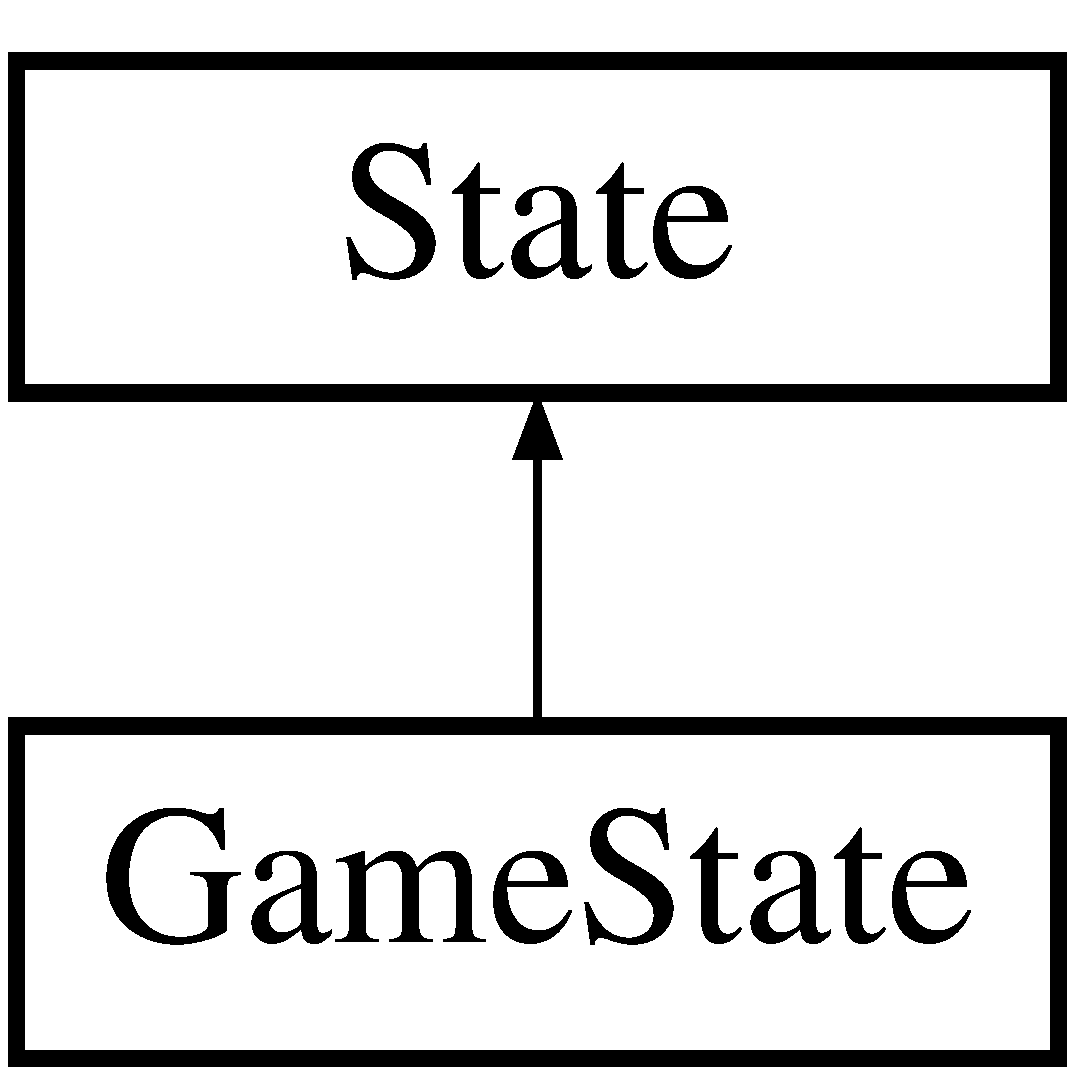
\includegraphics[height=2.000000cm]{class_game_state}
\end{center}
\end{figure}
\subsection*{Public Member Functions}
\begin{DoxyCompactItemize}
\item 
\hyperlink{class_game_state_a0e812c09d724c03147ad6721b4d7bd73}{Game\+State} (\hyperlink{class_state_manager}{State\+Manager} $\ast$, S\+D\+L\+\_\+\+Renderer $\ast$)
\item 
\hyperlink{class_game_state_ae623df5042cd0c17daa3394fdcb397b3}{$\sim$\+Game\+State} ()
\item 
bool \hyperlink{class_game_state_a5e2467775e9a941d482e0489295c363d}{Handle\+S\+D\+L\+Events} ()
\item 
void \hyperlink{class_game_state_a2ea32b0cd5f747ef6223d182f415a6c4}{Update} (float delta\+Time)
\item 
void \hyperlink{class_game_state_ab9330b36c7c74d733c2739c025285c64}{Draw} ()
\end{DoxyCompactItemize}
\subsection*{Additional Inherited Members}


\subsection{Detailed Description}
Creates a \hyperlink{class_game_state}{Game\+State} object. Creates a \hyperlink{class_game_state}{Game\+State} object that inherits \hyperlink{class_state}{State}. 

\subsection{Constructor \& Destructor Documentation}
\hypertarget{class_game_state_a0e812c09d724c03147ad6721b4d7bd73}{\index{Game\+State@{Game\+State}!Game\+State@{Game\+State}}
\index{Game\+State@{Game\+State}!Game\+State@{Game\+State}}
\subsubsection[{Game\+State}]{\setlength{\rightskip}{0pt plus 5cm}Game\+State\+::\+Game\+State (
\begin{DoxyParamCaption}
\item[{{\bf State\+Manager} $\ast$}]{in\+State\+Manager, }
\item[{S\+D\+L\+\_\+\+Renderer $\ast$}]{in\+Renderer}
\end{DoxyParamCaption}
)}}\label{class_game_state_a0e812c09d724c03147ad6721b4d7bd73}
Constructs a \hyperlink{class_game_state}{Game\+State} object Constructs a \hyperlink{class_game_state}{Game\+State} object 
\begin{DoxyParams}{Parameters}
{\em \hyperlink{class_state_manager}{State\+Manager}} & $\ast$ a pointer to the \hyperlink{class_state_manager}{State\+Manager} \\
\hline
{\em S\+D\+L\+\_\+\+Renderer} & $\ast$ a pointer to the renderer in use. \\
\hline
\end{DoxyParams}
\hypertarget{class_game_state_ae623df5042cd0c17daa3394fdcb397b3}{\index{Game\+State@{Game\+State}!````~Game\+State@{$\sim$\+Game\+State}}
\index{````~Game\+State@{$\sim$\+Game\+State}!Game\+State@{Game\+State}}
\subsubsection[{$\sim$\+Game\+State}]{\setlength{\rightskip}{0pt plus 5cm}Game\+State\+::$\sim$\+Game\+State (
\begin{DoxyParamCaption}
{}
\end{DoxyParamCaption}
)}}\label{class_game_state_ae623df5042cd0c17daa3394fdcb397b3}
De-\/constructs a \hyperlink{class_game_state}{Game\+State} object De-\/constructs the \hyperlink{class_game_state}{Game\+State} object 

\subsection{Member Function Documentation}
\hypertarget{class_game_state_ab9330b36c7c74d733c2739c025285c64}{\index{Game\+State@{Game\+State}!Draw@{Draw}}
\index{Draw@{Draw}!Game\+State@{Game\+State}}
\subsubsection[{Draw}]{\setlength{\rightskip}{0pt plus 5cm}void Game\+State\+::\+Draw (
\begin{DoxyParamCaption}
{}
\end{DoxyParamCaption}
)\hspace{0.3cm}{\ttfamily [virtual]}}}\label{class_game_state_ab9330b36c7c74d733c2739c025285c64}
A function to draw to the screen A function to draw to the screen using the renderer 

Implements \hyperlink{class_state_a8b0cdb0e7450a9bb3580a33dfbe4d981}{State}.

\hypertarget{class_game_state_a5e2467775e9a941d482e0489295c363d}{\index{Game\+State@{Game\+State}!Handle\+S\+D\+L\+Events@{Handle\+S\+D\+L\+Events}}
\index{Handle\+S\+D\+L\+Events@{Handle\+S\+D\+L\+Events}!Game\+State@{Game\+State}}
\subsubsection[{Handle\+S\+D\+L\+Events}]{\setlength{\rightskip}{0pt plus 5cm}bool Game\+State\+::\+Handle\+S\+D\+L\+Events (
\begin{DoxyParamCaption}
{}
\end{DoxyParamCaption}
)\hspace{0.3cm}{\ttfamily [virtual]}}}\label{class_game_state_a5e2467775e9a941d482e0489295c363d}
A function to handle the S\+D\+L events A function to handle the S\+D\+L events for use with the \hyperlink{class_game_state}{Game\+State} \begin{DoxyReturn}{Returns}
bool if false then quit \hyperlink{class_game_state}{Game\+State} 
\end{DoxyReturn}


Implements \hyperlink{class_state_a648d9182cab9aeb914ef778f94e2b437}{State}.

\hypertarget{class_game_state_a2ea32b0cd5f747ef6223d182f415a6c4}{\index{Game\+State@{Game\+State}!Update@{Update}}
\index{Update@{Update}!Game\+State@{Game\+State}}
\subsubsection[{Update}]{\setlength{\rightskip}{0pt plus 5cm}void Game\+State\+::\+Update (
\begin{DoxyParamCaption}
\item[{float}]{delta\+Time}
\end{DoxyParamCaption}
)\hspace{0.3cm}{\ttfamily [virtual]}}}\label{class_game_state_a2ea32b0cd5f747ef6223d182f415a6c4}
A function to update the \hyperlink{class_game_state}{Game\+State} A function to update the \hyperlink{class_game_state}{Game\+State} to allow the \hyperlink{class_game_state}{Game\+State} to run 
\begin{DoxyParams}{Parameters}
{\em float} & the delta time \\
\hline
\end{DoxyParams}


Implements \hyperlink{class_state_a770f40188fdfc64bc95a5166fef12e02}{State}.



The documentation for this class was generated from the following files\+:\begin{DoxyCompactItemize}
\item 
P\+G\+G\+Assignment1\+S\+D\+L/game\+State.\+h\item 
P\+G\+G\+Assignment1\+S\+D\+L/game\+State.\+cpp\end{DoxyCompactItemize}

\hypertarget{class_gem}{\section{Gem Class Reference}
\label{class_gem}\index{Gem@{Gem}}
}


Creates a \hyperlink{class_gem}{Gem} object that inherits \hyperlink{class_map_object}{Map\+Object}.  




{\ttfamily \#include $<$gem.\+h$>$}

Inheritance diagram for Gem\+:\begin{figure}[H]
\begin{center}
\leavevmode
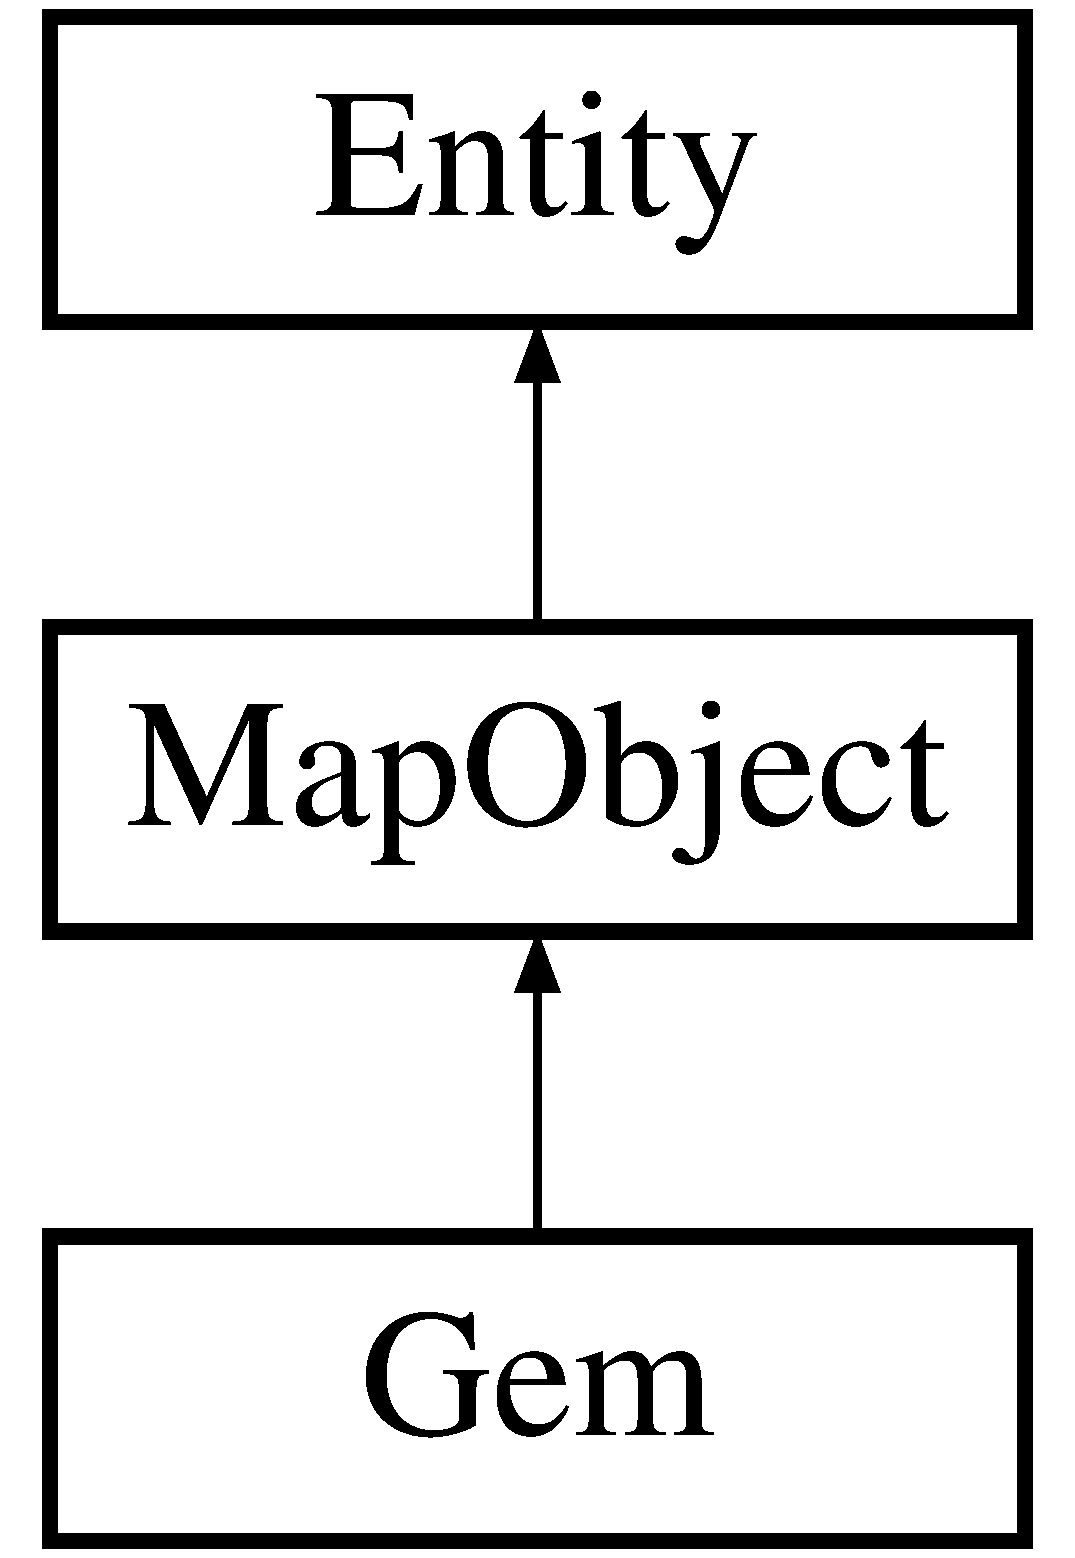
\includegraphics[height=3.000000cm]{class_gem}
\end{center}
\end{figure}
\subsection*{Public Member Functions}
\begin{DoxyCompactItemize}
\item 
\hyperlink{class_gem_a9b964b4eacf579f4e9fa2e6006222ca4}{Gem} (\hyperlink{class_texture}{Texture} $\ast$, float, float, int)
\item 
\hyperlink{class_gem_a25c24193733a5c4b9c230e4164b08cd4}{$\sim$\+Gem} ()
\item 
void \hyperlink{class_gem_a5b88637e9b62fc71af306f58f5c82cef}{type\+Setup} ()
\item 
int \hyperlink{class_gem_acccf14e79a3e6a9db263081e88e953e1}{get\+Value} ()
\item 
int \hyperlink{class_gem_afee29c071abd184ecaa5eb8925066691}{get\+Type} ()
\end{DoxyCompactItemize}
\subsection*{Additional Inherited Members}


\subsection{Detailed Description}
Creates a \hyperlink{class_gem}{Gem} object that inherits \hyperlink{class_map_object}{Map\+Object}. 

\subsection{Constructor \& Destructor Documentation}
\hypertarget{class_gem_a9b964b4eacf579f4e9fa2e6006222ca4}{\index{Gem@{Gem}!Gem@{Gem}}
\index{Gem@{Gem}!Gem@{Gem}}
\subsubsection[{Gem}]{\setlength{\rightskip}{0pt plus 5cm}Gem\+::\+Gem (
\begin{DoxyParamCaption}
\item[{{\bf Texture} $\ast$}]{input\+Texture, }
\item[{float}]{input\+X, }
\item[{float}]{input\+Y, }
\item[{int}]{in\+Type}
\end{DoxyParamCaption}
)}}\label{class_gem_a9b964b4eacf579f4e9fa2e6006222ca4}
Constructs a \hyperlink{class_gem}{Gem} object Constructs the \hyperlink{class_gem}{Gem} object. 
\begin{DoxyParams}{Parameters}
{\em Texture$\ast$} & a pointer to a \hyperlink{class_texture}{Texture} loaded into memory. \\
\hline
{\em float} & initial x position. \\
\hline
{\em float} & initial y position. \\
\hline
{\em int} & the \hyperlink{class_gem}{Gem} type. \\
\hline
\end{DoxyParams}
\hypertarget{class_gem_a25c24193733a5c4b9c230e4164b08cd4}{\index{Gem@{Gem}!````~Gem@{$\sim$\+Gem}}
\index{````~Gem@{$\sim$\+Gem}!Gem@{Gem}}
\subsubsection[{$\sim$\+Gem}]{\setlength{\rightskip}{0pt plus 5cm}Gem\+::$\sim$\+Gem (
\begin{DoxyParamCaption}
{}
\end{DoxyParamCaption}
)}}\label{class_gem_a25c24193733a5c4b9c230e4164b08cd4}
De-\/constructs a \hyperlink{class_gem}{Gem} object De-\/constructs the \hyperlink{class_gem}{Gem} object 

\subsection{Member Function Documentation}
\hypertarget{class_gem_afee29c071abd184ecaa5eb8925066691}{\index{Gem@{Gem}!get\+Type@{get\+Type}}
\index{get\+Type@{get\+Type}!Gem@{Gem}}
\subsubsection[{get\+Type}]{\setlength{\rightskip}{0pt plus 5cm}int Gem\+::get\+Type (
\begin{DoxyParamCaption}
{}
\end{DoxyParamCaption}
)}}\label{class_gem_afee29c071abd184ecaa5eb8925066691}
Getter \# type \begin{DoxyReturn}{Returns}
int the type. 
\end{DoxyReturn}
\hypertarget{class_gem_acccf14e79a3e6a9db263081e88e953e1}{\index{Gem@{Gem}!get\+Value@{get\+Value}}
\index{get\+Value@{get\+Value}!Gem@{Gem}}
\subsubsection[{get\+Value}]{\setlength{\rightskip}{0pt plus 5cm}int Gem\+::get\+Value (
\begin{DoxyParamCaption}
{}
\end{DoxyParamCaption}
)}}\label{class_gem_acccf14e79a3e6a9db263081e88e953e1}
Getter \# value \begin{DoxyReturn}{Returns}
int the value of the gem. 
\end{DoxyReturn}
\hypertarget{class_gem_a5b88637e9b62fc71af306f58f5c82cef}{\index{Gem@{Gem}!type\+Setup@{type\+Setup}}
\index{type\+Setup@{type\+Setup}!Gem@{Gem}}
\subsubsection[{type\+Setup}]{\setlength{\rightskip}{0pt plus 5cm}void Gem\+::type\+Setup (
\begin{DoxyParamCaption}
{}
\end{DoxyParamCaption}
)}}\label{class_gem_a5b88637e9b62fc71af306f58f5c82cef}
Sets the type of the \hyperlink{class_gem}{Gem} Uses the value of type to set up initial values for the \hyperlink{class_gem}{Gem} 

The documentation for this class was generated from the following files\+:\begin{DoxyCompactItemize}
\item 
P\+G\+G\+Assignment1\+S\+D\+L/gem.\+h\item 
P\+G\+G\+Assignment1\+S\+D\+L/gem.\+cpp\end{DoxyCompactItemize}

\hypertarget{class_help_state}{\section{Help\+State Class Reference}
\label{class_help_state}\index{Help\+State@{Help\+State}}
}


Creates a \hyperlink{class_help_state}{Help\+State} object. Creates a \hyperlink{class_help_state}{Help\+State} object that inherits \hyperlink{class_state}{State}.  




{\ttfamily \#include $<$help\+State.\+h$>$}



Inheritance diagram for Help\+State\+:
\nopagebreak
\begin{figure}[H]
\begin{center}
\leavevmode
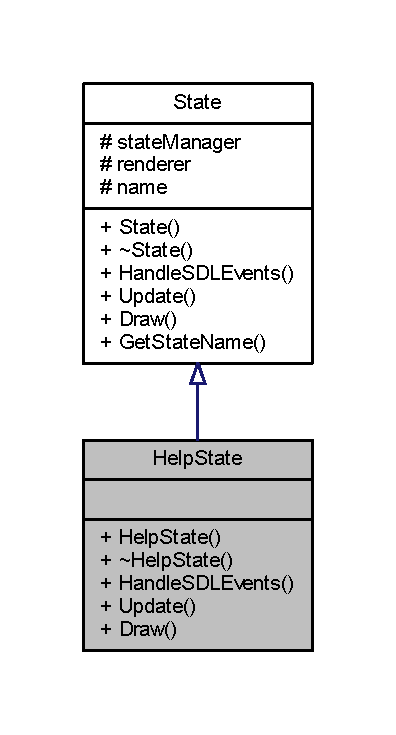
\includegraphics[width=190pt]{class_help_state__inherit__graph}
\end{center}
\end{figure}


Collaboration diagram for Help\+State\+:
\nopagebreak
\begin{figure}[H]
\begin{center}
\leavevmode
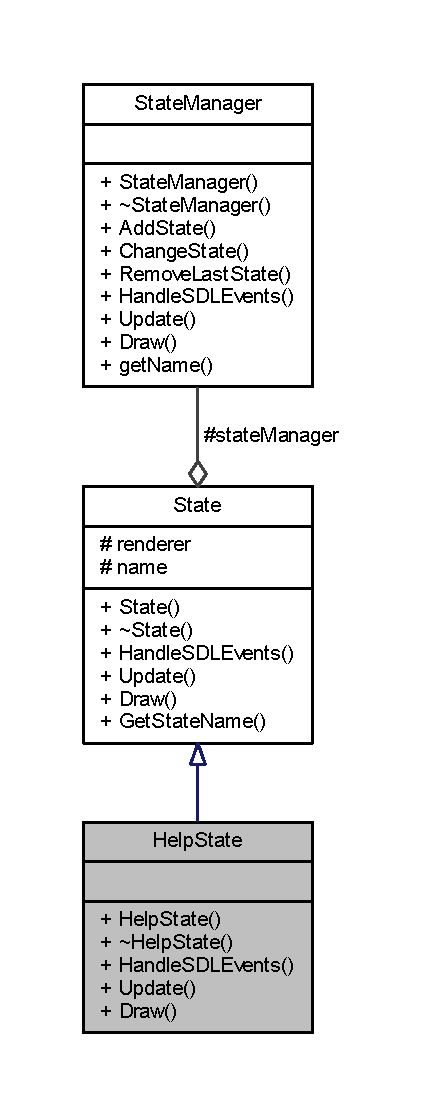
\includegraphics[width=203pt]{class_help_state__coll__graph}
\end{center}
\end{figure}
\subsection*{Public Member Functions}
\begin{DoxyCompactItemize}
\item 
\hyperlink{class_help_state_a2c988d45d9f13b048fa8e44ad4c49571}{Help\+State} (\hyperlink{class_state_manager}{State\+Manager} $\ast$, S\+D\+L\+\_\+\+Renderer $\ast$)
\item 
\hyperlink{class_help_state_a9698cf3f338866bcbd05ec25fa20700c}{$\sim$\+Help\+State} ()
\item 
bool \hyperlink{class_help_state_a7149e10e0129b66a68290d259bce3015}{Handle\+S\+D\+L\+Events} ()
\item 
void \hyperlink{class_help_state_ac9a45859141cae970629aac1e7a69184}{Update} (float delta\+Time)
\item 
void \hyperlink{class_help_state_a281d12605303cc444e600b214a8d2161}{Draw} ()
\end{DoxyCompactItemize}
\subsection*{Additional Inherited Members}


\subsection{Detailed Description}
Creates a \hyperlink{class_help_state}{Help\+State} object. Creates a \hyperlink{class_help_state}{Help\+State} object that inherits \hyperlink{class_state}{State}. 

\subsection{Constructor \& Destructor Documentation}
\hypertarget{class_help_state_a2c988d45d9f13b048fa8e44ad4c49571}{\index{Help\+State@{Help\+State}!Help\+State@{Help\+State}}
\index{Help\+State@{Help\+State}!Help\+State@{Help\+State}}
\subsubsection[{Help\+State}]{\setlength{\rightskip}{0pt plus 5cm}Help\+State\+::\+Help\+State (
\begin{DoxyParamCaption}
\item[{{\bf State\+Manager} $\ast$}]{in\+State\+Manager, }
\item[{S\+D\+L\+\_\+\+Renderer $\ast$}]{in\+Renderer}
\end{DoxyParamCaption}
)}}\label{class_help_state_a2c988d45d9f13b048fa8e44ad4c49571}
Constructs a \hyperlink{class_help_state}{Help\+State} object Constructs a \hyperlink{class_help_state}{Help\+State} object 
\begin{DoxyParams}{Parameters}
{\em \hyperlink{class_state_manager}{State\+Manager}} & $\ast$ a pointer to the \hyperlink{class_state_manager}{State\+Manager} \\
\hline
{\em S\+D\+L\+\_\+\+Renderer} & $\ast$ a pointer to the renderer in use. \\
\hline
\end{DoxyParams}
\hypertarget{class_help_state_a9698cf3f338866bcbd05ec25fa20700c}{\index{Help\+State@{Help\+State}!````~Help\+State@{$\sim$\+Help\+State}}
\index{````~Help\+State@{$\sim$\+Help\+State}!Help\+State@{Help\+State}}
\subsubsection[{$\sim$\+Help\+State}]{\setlength{\rightskip}{0pt plus 5cm}Help\+State\+::$\sim$\+Help\+State (
\begin{DoxyParamCaption}
{}
\end{DoxyParamCaption}
)}}\label{class_help_state_a9698cf3f338866bcbd05ec25fa20700c}
De-\/constructs a \hyperlink{class_help_state}{Help\+State} object De-\/constructs the \hyperlink{class_help_state}{Help\+State} object 

\subsection{Member Function Documentation}
\hypertarget{class_help_state_a281d12605303cc444e600b214a8d2161}{\index{Help\+State@{Help\+State}!Draw@{Draw}}
\index{Draw@{Draw}!Help\+State@{Help\+State}}
\subsubsection[{Draw}]{\setlength{\rightskip}{0pt plus 5cm}void Help\+State\+::\+Draw (
\begin{DoxyParamCaption}
{}
\end{DoxyParamCaption}
)\hspace{0.3cm}{\ttfamily [virtual]}}}\label{class_help_state_a281d12605303cc444e600b214a8d2161}
A function to draw to the screen A function to draw to the screen using the renderer 

Implements \hyperlink{class_state_a8b0cdb0e7450a9bb3580a33dfbe4d981}{State}.



Here is the call graph for this function\+:
\nopagebreak
\begin{figure}[H]
\begin{center}
\leavevmode
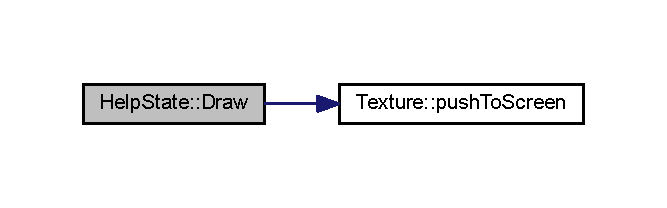
\includegraphics[width=320pt]{class_help_state_a281d12605303cc444e600b214a8d2161_cgraph}
\end{center}
\end{figure}


\hypertarget{class_help_state_a7149e10e0129b66a68290d259bce3015}{\index{Help\+State@{Help\+State}!Handle\+S\+D\+L\+Events@{Handle\+S\+D\+L\+Events}}
\index{Handle\+S\+D\+L\+Events@{Handle\+S\+D\+L\+Events}!Help\+State@{Help\+State}}
\subsubsection[{Handle\+S\+D\+L\+Events}]{\setlength{\rightskip}{0pt plus 5cm}bool Help\+State\+::\+Handle\+S\+D\+L\+Events (
\begin{DoxyParamCaption}
{}
\end{DoxyParamCaption}
)\hspace{0.3cm}{\ttfamily [virtual]}}}\label{class_help_state_a7149e10e0129b66a68290d259bce3015}
A function to handle the S\+D\+L events A function to handle the S\+D\+L events for use with the \hyperlink{class_help_state}{Help\+State} \begin{DoxyReturn}{Returns}
bool if false then quit \hyperlink{class_help_state}{Help\+State} 
\end{DoxyReturn}


Implements \hyperlink{class_state_a648d9182cab9aeb914ef778f94e2b437}{State}.



Here is the call graph for this function\+:
\nopagebreak
\begin{figure}[H]
\begin{center}
\leavevmode
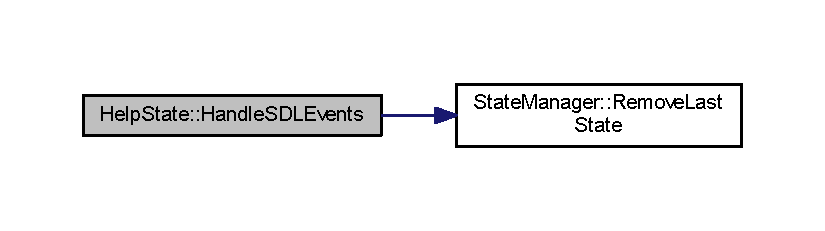
\includegraphics[width=350pt]{class_help_state_a7149e10e0129b66a68290d259bce3015_cgraph}
\end{center}
\end{figure}


\hypertarget{class_help_state_ac9a45859141cae970629aac1e7a69184}{\index{Help\+State@{Help\+State}!Update@{Update}}
\index{Update@{Update}!Help\+State@{Help\+State}}
\subsubsection[{Update}]{\setlength{\rightskip}{0pt plus 5cm}void Help\+State\+::\+Update (
\begin{DoxyParamCaption}
\item[{float}]{delta\+Time}
\end{DoxyParamCaption}
)\hspace{0.3cm}{\ttfamily [virtual]}}}\label{class_help_state_ac9a45859141cae970629aac1e7a69184}
A function to update the \hyperlink{class_help_state}{Help\+State} A function to update the \hyperlink{class_help_state}{Help\+State} to allow the \hyperlink{class_help_state}{Help\+State} to run 
\begin{DoxyParams}{Parameters}
{\em float} & the delta time \\
\hline
\end{DoxyParams}


Implements \hyperlink{class_state_a770f40188fdfc64bc95a5166fef12e02}{State}.



The documentation for this class was generated from the following files\+:\begin{DoxyCompactItemize}
\item 
P\+G\+G\+Assignment1\+S\+D\+L/help\+State.\+h\item 
P\+G\+G\+Assignment1\+S\+D\+L/help\+State.\+cpp\end{DoxyCompactItemize}

\hypertarget{class_map_loader}{\section{Map\+Loader Class Reference}
\label{class_map_loader}\index{Map\+Loader@{Map\+Loader}}
}


a class to load in a map text file  




{\ttfamily \#include $<$map\+Loader.\+h$>$}

\subsection*{Public Member Functions}
\begin{DoxyCompactItemize}
\item 
\hyperlink{class_map_loader_a759260eb5a2bcc71f4eb6e03e8d8dead}{Map\+Loader} (std\+::string, \hyperlink{class_texture}{Texture} $\ast$, int)
\item 
\hyperlink{class_map_loader_a6055310649b9a926301d7fb2b83cb1b1}{$\sim$\+Map\+Loader} ()
\item 
void \hyperlink{class_map_loader_aa3f95e47879ef5d2ac8f9b4e80602412}{load\+Map} (std\+::string, int)
\item 
void \hyperlink{class_map_loader_a5d094d7c804670f68e04c360cb9b5965}{sort\+Type} (int, int, int, int)
\item 
void \hyperlink{class_map_loader_a0430f4acdbe19fd6853a61e3b9f71543}{display\+Block} (int, S\+D\+L\+\_\+\+Renderer $\ast$)
\item 
void \hyperlink{class_map_loader_adf524d17cab14e1096341100abfe92b2}{display\+Gem} (int, S\+D\+L\+\_\+\+Renderer $\ast$)
\item 
int \hyperlink{class_map_loader_a178ca855ceec126f0a3a2264b74f63cc}{get\+Number\+Of\+Blocks} ()
\item 
int \hyperlink{class_map_loader_a026a7c38e03cdee9a355b09ca6048daa}{get\+Numberof\+Gems} ()
\item 
\hyperlink{class_block}{Block} $\ast$ \hyperlink{class_map_loader_a161a0cc6a392abc9baa57e919023f25c}{get\+Block} (int)
\item 
\hyperlink{class_gem}{Gem} $\ast$ \hyperlink{class_map_loader_a9b56fda5f4c27614131b085b449fe183}{get\+Gem} (int)
\end{DoxyCompactItemize}


\subsection{Detailed Description}
a class to load in a map text file 

\subsection{Constructor \& Destructor Documentation}
\hypertarget{class_map_loader_a759260eb5a2bcc71f4eb6e03e8d8dead}{\index{Map\+Loader@{Map\+Loader}!Map\+Loader@{Map\+Loader}}
\index{Map\+Loader@{Map\+Loader}!Map\+Loader@{Map\+Loader}}
\subsubsection[{Map\+Loader}]{\setlength{\rightskip}{0pt plus 5cm}Map\+Loader\+::\+Map\+Loader (
\begin{DoxyParamCaption}
\item[{std\+::string}]{file\+Name, }
\item[{{\bf Texture} $\ast$}]{in\+Texture, }
\item[{int}]{background\+Type}
\end{DoxyParamCaption}
)}}\label{class_map_loader_a759260eb5a2bcc71f4eb6e03e8d8dead}
Constructs \hyperlink{class_map_loader}{Map\+Loader} object Constructs a \hyperlink{class_map_loader}{Map\+Loader} object. 
\begin{DoxyParams}{Parameters}
{\em std\+::string} & the file location \\
\hline
{\em \hyperlink{class_texture}{Texture}} & $\ast$ a pointer to the spritesheet \\
\hline
{\em int} & the type of background \\
\hline
\end{DoxyParams}
\hypertarget{class_map_loader_a6055310649b9a926301d7fb2b83cb1b1}{\index{Map\+Loader@{Map\+Loader}!````~Map\+Loader@{$\sim$\+Map\+Loader}}
\index{````~Map\+Loader@{$\sim$\+Map\+Loader}!Map\+Loader@{Map\+Loader}}
\subsubsection[{$\sim$\+Map\+Loader}]{\setlength{\rightskip}{0pt plus 5cm}Map\+Loader\+::$\sim$\+Map\+Loader (
\begin{DoxyParamCaption}
{}
\end{DoxyParamCaption}
)}}\label{class_map_loader_a6055310649b9a926301d7fb2b83cb1b1}
De-\/constructs a \hyperlink{class_map_loader}{Map\+Loader} object De-\/constructs the \hyperlink{class_map_loader}{Map\+Loader} object 

\subsection{Member Function Documentation}
\hypertarget{class_map_loader_a0430f4acdbe19fd6853a61e3b9f71543}{\index{Map\+Loader@{Map\+Loader}!display\+Block@{display\+Block}}
\index{display\+Block@{display\+Block}!Map\+Loader@{Map\+Loader}}
\subsubsection[{display\+Block}]{\setlength{\rightskip}{0pt plus 5cm}void Map\+Loader\+::display\+Block (
\begin{DoxyParamCaption}
\item[{int}]{i, }
\item[{S\+D\+L\+\_\+\+Renderer $\ast$}]{renderer}
\end{DoxyParamCaption}
)}}\label{class_map_loader_a0430f4acdbe19fd6853a61e3b9f71543}
display the \hyperlink{class_block}{Block} object display the \hyperlink{class_block}{Block} at the position at the array inputed 
\begin{DoxyParams}{Parameters}
{\em int} & the index of the \hyperlink{class_block}{Block} array \\
\hline
{\em S\+D\+L\+\_\+\+Renderer} & $\ast$ a pointer to the renderer \\
\hline
\end{DoxyParams}
\hypertarget{class_map_loader_adf524d17cab14e1096341100abfe92b2}{\index{Map\+Loader@{Map\+Loader}!display\+Gem@{display\+Gem}}
\index{display\+Gem@{display\+Gem}!Map\+Loader@{Map\+Loader}}
\subsubsection[{display\+Gem}]{\setlength{\rightskip}{0pt plus 5cm}void Map\+Loader\+::display\+Gem (
\begin{DoxyParamCaption}
\item[{int}]{i, }
\item[{S\+D\+L\+\_\+\+Renderer $\ast$}]{renderer}
\end{DoxyParamCaption}
)}}\label{class_map_loader_adf524d17cab14e1096341100abfe92b2}
display the \hyperlink{class_gem}{Gem} object display the \hyperlink{class_gem}{Gem} at the position at the array inputed 
\begin{DoxyParams}{Parameters}
{\em int} & the index of the \hyperlink{class_gem}{Gem} array \\
\hline
{\em S\+D\+L\+\_\+\+Renderer} & $\ast$ a pointer to the renderer \\
\hline
\end{DoxyParams}
\hypertarget{class_map_loader_a161a0cc6a392abc9baa57e919023f25c}{\index{Map\+Loader@{Map\+Loader}!get\+Block@{get\+Block}}
\index{get\+Block@{get\+Block}!Map\+Loader@{Map\+Loader}}
\subsubsection[{get\+Block}]{\setlength{\rightskip}{0pt plus 5cm}{\bf Block} $\ast$ Map\+Loader\+::get\+Block (
\begin{DoxyParamCaption}
\item[{int}]{i}
\end{DoxyParamCaption}
)}}\label{class_map_loader_a161a0cc6a392abc9baa57e919023f25c}
Getter \# a \hyperlink{class_block}{Block} from the array 
\begin{DoxyParams}{Parameters}
{\em int} & the index of the block \\
\hline
\end{DoxyParams}
\begin{DoxyReturn}{Returns}
a pointer to a \hyperlink{class_block}{Block}. 
\end{DoxyReturn}
\hypertarget{class_map_loader_a9b56fda5f4c27614131b085b449fe183}{\index{Map\+Loader@{Map\+Loader}!get\+Gem@{get\+Gem}}
\index{get\+Gem@{get\+Gem}!Map\+Loader@{Map\+Loader}}
\subsubsection[{get\+Gem}]{\setlength{\rightskip}{0pt plus 5cm}{\bf Gem} $\ast$ Map\+Loader\+::get\+Gem (
\begin{DoxyParamCaption}
\item[{int}]{i}
\end{DoxyParamCaption}
)}}\label{class_map_loader_a9b56fda5f4c27614131b085b449fe183}
Getter \# a \hyperlink{class_block}{Block} from the array 
\begin{DoxyParams}{Parameters}
{\em int} & the index of the block \\
\hline
\end{DoxyParams}
\begin{DoxyReturn}{Returns}
a pointer to a \hyperlink{class_block}{Block}. 
\end{DoxyReturn}
\hypertarget{class_map_loader_a178ca855ceec126f0a3a2264b74f63cc}{\index{Map\+Loader@{Map\+Loader}!get\+Number\+Of\+Blocks@{get\+Number\+Of\+Blocks}}
\index{get\+Number\+Of\+Blocks@{get\+Number\+Of\+Blocks}!Map\+Loader@{Map\+Loader}}
\subsubsection[{get\+Number\+Of\+Blocks}]{\setlength{\rightskip}{0pt plus 5cm}int Map\+Loader\+::get\+Number\+Of\+Blocks (
\begin{DoxyParamCaption}
{}
\end{DoxyParamCaption}
)}}\label{class_map_loader_a178ca855ceec126f0a3a2264b74f63cc}
Getter \# number of blocks \begin{DoxyReturn}{Returns}
the number of blocks. 
\end{DoxyReturn}
\hypertarget{class_map_loader_a026a7c38e03cdee9a355b09ca6048daa}{\index{Map\+Loader@{Map\+Loader}!get\+Numberof\+Gems@{get\+Numberof\+Gems}}
\index{get\+Numberof\+Gems@{get\+Numberof\+Gems}!Map\+Loader@{Map\+Loader}}
\subsubsection[{get\+Numberof\+Gems}]{\setlength{\rightskip}{0pt plus 5cm}int Map\+Loader\+::get\+Numberof\+Gems (
\begin{DoxyParamCaption}
{}
\end{DoxyParamCaption}
)}}\label{class_map_loader_a026a7c38e03cdee9a355b09ca6048daa}
Getter \# height \begin{DoxyReturn}{Returns}
the number of gems. 
\end{DoxyReturn}
\hypertarget{class_map_loader_aa3f95e47879ef5d2ac8f9b4e80602412}{\index{Map\+Loader@{Map\+Loader}!load\+Map@{load\+Map}}
\index{load\+Map@{load\+Map}!Map\+Loader@{Map\+Loader}}
\subsubsection[{load\+Map}]{\setlength{\rightskip}{0pt plus 5cm}void Map\+Loader\+::load\+Map (
\begin{DoxyParamCaption}
\item[{std\+::string}]{file\+Name, }
\item[{int}]{background\+Type}
\end{DoxyParamCaption}
)}}\label{class_map_loader_aa3f95e47879ef5d2ac8f9b4e80602412}
load the map file load the map file from the location passed in. 
\begin{DoxyParams}{Parameters}
{\em std\+::string} & the file location \\
\hline
{\em int} & the type of background \\
\hline
\end{DoxyParams}
\hypertarget{class_map_loader_a5d094d7c804670f68e04c360cb9b5965}{\index{Map\+Loader@{Map\+Loader}!sort\+Type@{sort\+Type}}
\index{sort\+Type@{sort\+Type}!Map\+Loader@{Map\+Loader}}
\subsubsection[{sort\+Type}]{\setlength{\rightskip}{0pt plus 5cm}void Map\+Loader\+::sort\+Type (
\begin{DoxyParamCaption}
\item[{int}]{type, }
\item[{int}]{i, }
\item[{int}]{j, }
\item[{int}]{background\+Type}
\end{DoxyParamCaption}
)}}\label{class_map_loader_a5d094d7c804670f68e04c360cb9b5965}
sort the map file object types take in the value of the current loaded type and declare the current map object to its correct type. 
\begin{DoxyParams}{Parameters}
{\em int} & the type of the object \\
\hline
{\em int} & the i index for the x position \\
\hline
{\em int} & the j index for the y position \\
\hline
{\em int} & the type of background \\
\hline
\end{DoxyParams}


The documentation for this class was generated from the following files\+:\begin{DoxyCompactItemize}
\item 
P\+G\+G\+Assignment1\+S\+D\+L/map\+Loader.\+h\item 
P\+G\+G\+Assignment1\+S\+D\+L/map\+Loader.\+cpp\end{DoxyCompactItemize}

\hypertarget{class_map_object}{\section{Map\+Object Class Reference}
\label{class_map_object}\index{Map\+Object@{Map\+Object}}
}


Creates a \hyperlink{class_map_object}{Map\+Object} object that inherits \hyperlink{class_entity}{Entity}.  




{\ttfamily \#include $<$map\+Object.\+h$>$}

Inheritance diagram for Map\+Object\+:\begin{figure}[H]
\begin{center}
\leavevmode
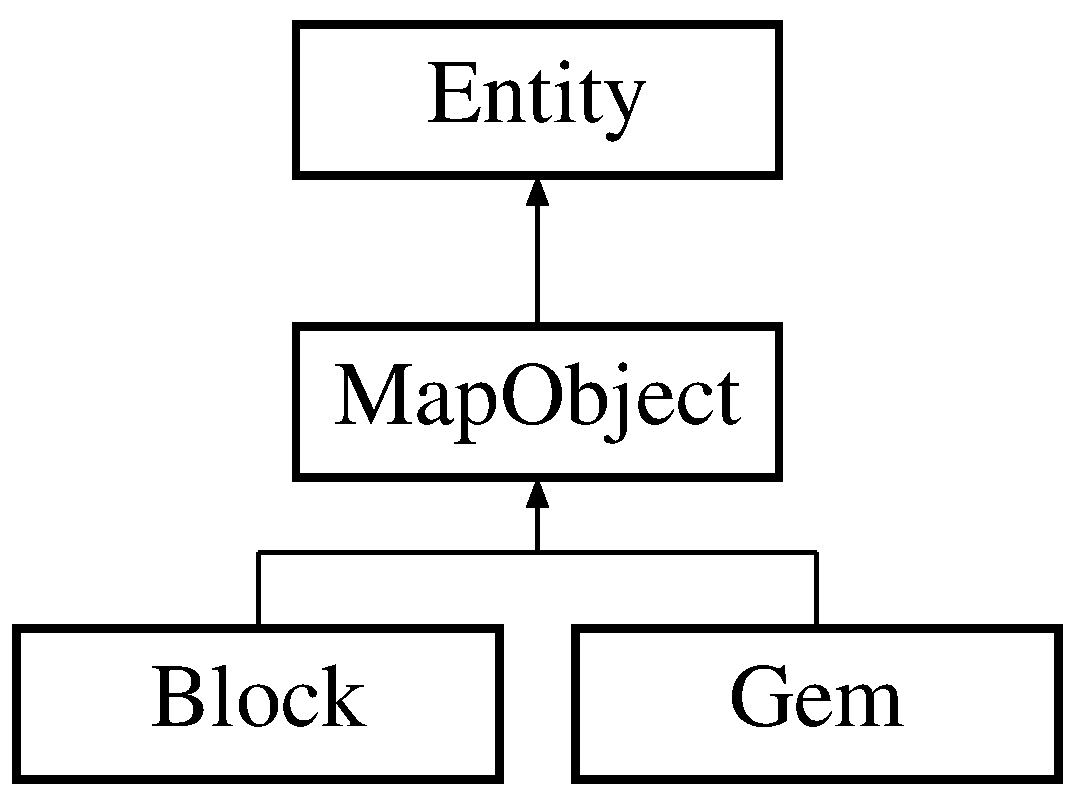
\includegraphics[height=3.000000cm]{class_map_object}
\end{center}
\end{figure}
\subsection*{Public Member Functions}
\begin{DoxyCompactItemize}
\item 
\hyperlink{class_map_object_a568754515cc72ce0861d30c3040d26d2}{Map\+Object} ()
\item 
\hyperlink{class_map_object_aa601344267a49df197e841fcbd732209}{$\sim$\+Map\+Object} ()
\item 
void \hyperlink{class_map_object_afc35a1271fdb83198e239a548b26337e}{set\+Collidable} (bool)
\item 
bool \hyperlink{class_map_object_a5c940048e408308c71b57a78444d155d}{get\+Collidable} ()
\item 
void \hyperlink{class_map_object_abcf8499f40944338e194abcbd3294852}{set\+Damaging} (bool)
\item 
bool \hyperlink{class_map_object_acaa0fff07bd2550c1f023ca90e2a4b04}{get\+Damaging} ()
\item 
void \hyperlink{class_map_object_af14721fd27162d9fd0f04f69d8087811}{set\+Deletable} (bool)
\item 
bool \hyperlink{class_map_object_a739bba3a3a50a84bf5e6244d19152a38}{get\+Deletable} ()
\end{DoxyCompactItemize}
\subsection*{Protected Attributes}
\begin{DoxyCompactItemize}
\item 
\hypertarget{class_map_object_a1d900ea8b9825881d5116711569b5e11}{bool {\bfseries collidable}}\label{class_map_object_a1d900ea8b9825881d5116711569b5e11}

\item 
\hypertarget{class_map_object_aa7f81dc2db7b5cdf0267717dee175d62}{bool {\bfseries damaging}}\label{class_map_object_aa7f81dc2db7b5cdf0267717dee175d62}

\item 
\hypertarget{class_map_object_a9c72b4c12be7a1b9c26adb3cfa10f029}{bool {\bfseries deleteable}}\label{class_map_object_a9c72b4c12be7a1b9c26adb3cfa10f029}

\end{DoxyCompactItemize}


\subsection{Detailed Description}
Creates a \hyperlink{class_map_object}{Map\+Object} object that inherits \hyperlink{class_entity}{Entity}. 

\subsection{Constructor \& Destructor Documentation}
\hypertarget{class_map_object_a568754515cc72ce0861d30c3040d26d2}{\index{Map\+Object@{Map\+Object}!Map\+Object@{Map\+Object}}
\index{Map\+Object@{Map\+Object}!Map\+Object@{Map\+Object}}
\subsubsection[{Map\+Object}]{\setlength{\rightskip}{0pt plus 5cm}Map\+Object\+::\+Map\+Object (
\begin{DoxyParamCaption}
{}
\end{DoxyParamCaption}
)}}\label{class_map_object_a568754515cc72ce0861d30c3040d26d2}
Constructs \hyperlink{class_map_object}{Map\+Object} object Constructs a \hyperlink{class_map_object}{Map\+Object} object. \hypertarget{class_map_object_aa601344267a49df197e841fcbd732209}{\index{Map\+Object@{Map\+Object}!````~Map\+Object@{$\sim$\+Map\+Object}}
\index{````~Map\+Object@{$\sim$\+Map\+Object}!Map\+Object@{Map\+Object}}
\subsubsection[{$\sim$\+Map\+Object}]{\setlength{\rightskip}{0pt plus 5cm}Map\+Object\+::$\sim$\+Map\+Object (
\begin{DoxyParamCaption}
{}
\end{DoxyParamCaption}
)}}\label{class_map_object_aa601344267a49df197e841fcbd732209}
De-\/constructs a \hyperlink{class_map_object}{Map\+Object} object De-\/constructs the \hyperlink{class_map_object}{Map\+Object} object 

\subsection{Member Function Documentation}
\hypertarget{class_map_object_a5c940048e408308c71b57a78444d155d}{\index{Map\+Object@{Map\+Object}!get\+Collidable@{get\+Collidable}}
\index{get\+Collidable@{get\+Collidable}!Map\+Object@{Map\+Object}}
\subsubsection[{get\+Collidable}]{\setlength{\rightskip}{0pt plus 5cm}bool Map\+Object\+::get\+Collidable (
\begin{DoxyParamCaption}
{}
\end{DoxyParamCaption}
)}}\label{class_map_object_a5c940048e408308c71b57a78444d155d}
Getter \# collidable Gets if the object is collidable \begin{DoxyReturn}{Returns}
bool if the map\+Object is collidable. 
\end{DoxyReturn}
\hypertarget{class_map_object_acaa0fff07bd2550c1f023ca90e2a4b04}{\index{Map\+Object@{Map\+Object}!get\+Damaging@{get\+Damaging}}
\index{get\+Damaging@{get\+Damaging}!Map\+Object@{Map\+Object}}
\subsubsection[{get\+Damaging}]{\setlength{\rightskip}{0pt plus 5cm}bool Map\+Object\+::get\+Damaging (
\begin{DoxyParamCaption}
{}
\end{DoxyParamCaption}
)}}\label{class_map_object_acaa0fff07bd2550c1f023ca90e2a4b04}
Getter \# damaging \begin{DoxyReturn}{Returns}
bool if the object causes damaging to the player. 
\end{DoxyReturn}
\hypertarget{class_map_object_a739bba3a3a50a84bf5e6244d19152a38}{\index{Map\+Object@{Map\+Object}!get\+Deletable@{get\+Deletable}}
\index{get\+Deletable@{get\+Deletable}!Map\+Object@{Map\+Object}}
\subsubsection[{get\+Deletable}]{\setlength{\rightskip}{0pt plus 5cm}bool Map\+Object\+::get\+Deletable (
\begin{DoxyParamCaption}
{}
\end{DoxyParamCaption}
)}}\label{class_map_object_a739bba3a3a50a84bf5e6244d19152a38}
Getter \# deleteable \begin{DoxyReturn}{Returns}
bool does the object need deleting. 
\end{DoxyReturn}
\hypertarget{class_map_object_afc35a1271fdb83198e239a548b26337e}{\index{Map\+Object@{Map\+Object}!set\+Collidable@{set\+Collidable}}
\index{set\+Collidable@{set\+Collidable}!Map\+Object@{Map\+Object}}
\subsubsection[{set\+Collidable}]{\setlength{\rightskip}{0pt plus 5cm}void Map\+Object\+::set\+Collidable (
\begin{DoxyParamCaption}
\item[{bool}]{input\+Collidable}
\end{DoxyParamCaption}
)}}\label{class_map_object_afc35a1271fdb83198e239a548b26337e}
Setter \# collidable Sets if the object is able to be collided with. 
\begin{DoxyParams}{Parameters}
{\em bool} & the collision boolean \\
\hline
\end{DoxyParams}
\hypertarget{class_map_object_abcf8499f40944338e194abcbd3294852}{\index{Map\+Object@{Map\+Object}!set\+Damaging@{set\+Damaging}}
\index{set\+Damaging@{set\+Damaging}!Map\+Object@{Map\+Object}}
\subsubsection[{set\+Damaging}]{\setlength{\rightskip}{0pt plus 5cm}void Map\+Object\+::set\+Damaging (
\begin{DoxyParamCaption}
\item[{bool}]{input\+Damaging}
\end{DoxyParamCaption}
)}}\label{class_map_object_abcf8499f40944338e194abcbd3294852}
Setter \# damaging Sets if the object causes damaging to the player. 
\begin{DoxyParams}{Parameters}
{\em bool} & the object causes damaging to the player. \\
\hline
\end{DoxyParams}
\hypertarget{class_map_object_af14721fd27162d9fd0f04f69d8087811}{\index{Map\+Object@{Map\+Object}!set\+Deletable@{set\+Deletable}}
\index{set\+Deletable@{set\+Deletable}!Map\+Object@{Map\+Object}}
\subsubsection[{set\+Deletable}]{\setlength{\rightskip}{0pt plus 5cm}void Map\+Object\+::set\+Deletable (
\begin{DoxyParamCaption}
\item[{bool}]{input\+Delete}
\end{DoxyParamCaption}
)}}\label{class_map_object_af14721fd27162d9fd0f04f69d8087811}
Setter \# deleteable Sets if the object needs to be deleted. 
\begin{DoxyParams}{Parameters}
{\em bool} & does the object need deleting. \\
\hline
\end{DoxyParams}


The documentation for this class was generated from the following files\+:\begin{DoxyCompactItemize}
\item 
P\+G\+G\+Assignment1\+S\+D\+L/map\+Object.\+h\item 
P\+G\+G\+Assignment1\+S\+D\+L/map\+Object.\+cpp\end{DoxyCompactItemize}

\hypertarget{class_menu_state}{\section{Menu\+State Class Reference}
\label{class_menu_state}\index{Menu\+State@{Menu\+State}}
}


Creates a \hyperlink{class_menu_state}{Menu\+State} object. Creates a \hyperlink{class_menu_state}{Menu\+State} object that inherits \hyperlink{class_state}{State}.  




{\ttfamily \#include $<$menu\+State.\+h$>$}

Inheritance diagram for Menu\+State\+:\begin{figure}[H]
\begin{center}
\leavevmode
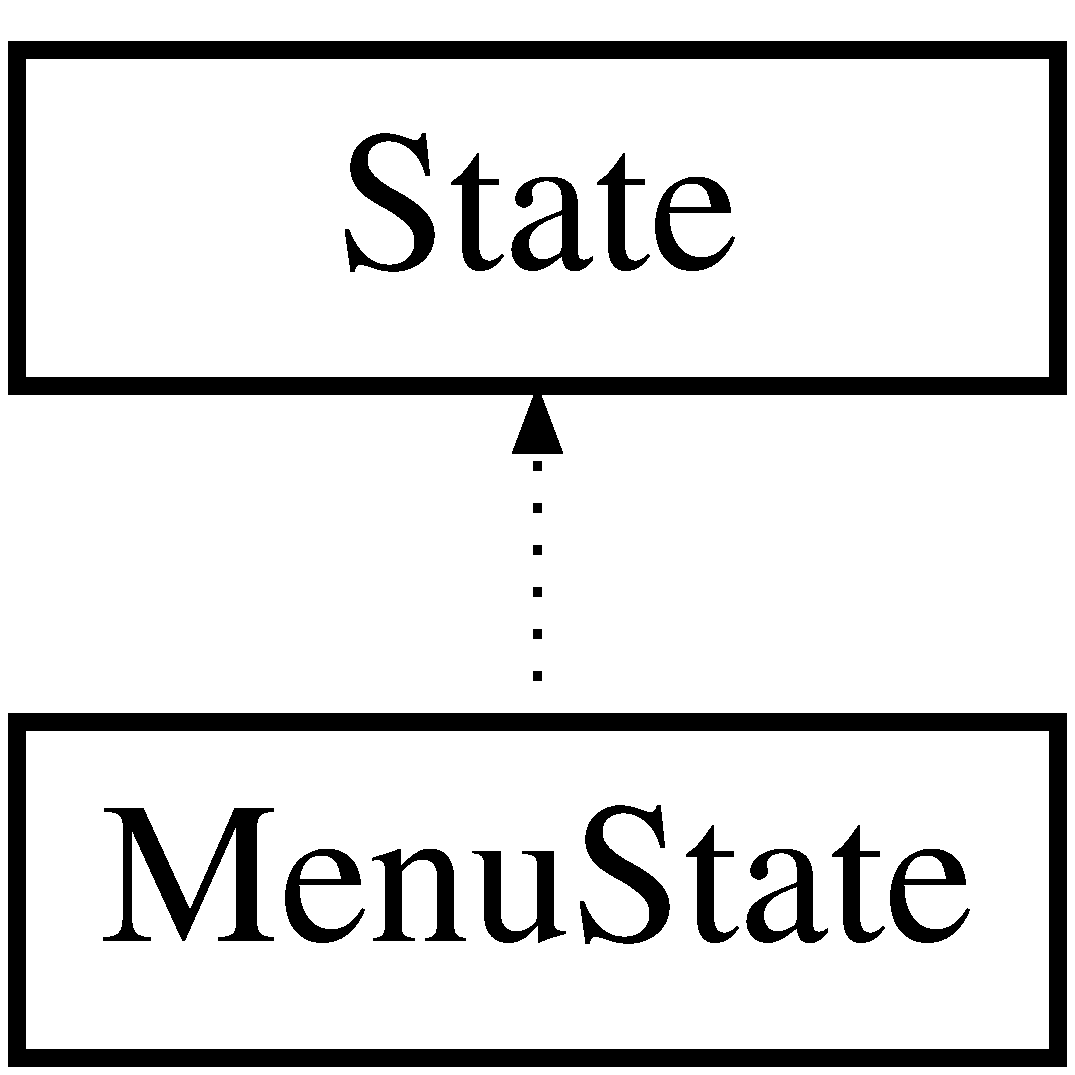
\includegraphics[height=2.000000cm]{class_menu_state}
\end{center}
\end{figure}
\subsection*{Public Member Functions}
\begin{DoxyCompactItemize}
\item 
\hyperlink{class_menu_state_a0cfcaba0ed63cdbcaf2d517e6bfbd2a2}{Menu\+State} (\hyperlink{class_state_manager}{State\+Manager} $\ast$, S\+D\+L\+\_\+\+Renderer $\ast$)
\item 
\hyperlink{class_menu_state_a58aea91a44436c5bba575c5de755a5bc}{$\sim$\+Menu\+State} ()
\item 
bool \hyperlink{class_menu_state_abab3b8017d47c6d6134cbdfb8e0c7580}{Handle\+S\+D\+L\+Events} ()
\item 
void \hyperlink{class_menu_state_a2ee9793bd50c42d8c7ce4cab62fbeba6}{Update} (float delta\+Time)
\item 
void \hyperlink{class_menu_state_a0fc92c6a39ef316552f1308c188871c6}{Draw} ()
\end{DoxyCompactItemize}
\subsection*{Additional Inherited Members}


\subsection{Detailed Description}
Creates a \hyperlink{class_menu_state}{Menu\+State} object. Creates a \hyperlink{class_menu_state}{Menu\+State} object that inherits \hyperlink{class_state}{State}. 

\subsection{Constructor \& Destructor Documentation}
\hypertarget{class_menu_state_a0cfcaba0ed63cdbcaf2d517e6bfbd2a2}{\index{Menu\+State@{Menu\+State}!Menu\+State@{Menu\+State}}
\index{Menu\+State@{Menu\+State}!Menu\+State@{Menu\+State}}
\subsubsection[{Menu\+State}]{\setlength{\rightskip}{0pt plus 5cm}Menu\+State\+::\+Menu\+State (
\begin{DoxyParamCaption}
\item[{{\bf State\+Manager} $\ast$}]{in\+State\+Manager, }
\item[{S\+D\+L\+\_\+\+Renderer $\ast$}]{renderer}
\end{DoxyParamCaption}
)}}\label{class_menu_state_a0cfcaba0ed63cdbcaf2d517e6bfbd2a2}
Constructs a \hyperlink{class_menu_state}{Menu\+State} object Constructs a \hyperlink{class_menu_state}{Menu\+State} object 
\begin{DoxyParams}{Parameters}
{\em \hyperlink{class_state_manager}{State\+Manager}} & $\ast$ a pointer to the \hyperlink{class_state_manager}{State\+Manager} \\
\hline
{\em S\+D\+L\+\_\+\+Renderer} & $\ast$ a pointer to the renderer in use. \\
\hline
\end{DoxyParams}
\hypertarget{class_menu_state_a58aea91a44436c5bba575c5de755a5bc}{\index{Menu\+State@{Menu\+State}!````~Menu\+State@{$\sim$\+Menu\+State}}
\index{````~Menu\+State@{$\sim$\+Menu\+State}!Menu\+State@{Menu\+State}}
\subsubsection[{$\sim$\+Menu\+State}]{\setlength{\rightskip}{0pt plus 5cm}Menu\+State\+::$\sim$\+Menu\+State (
\begin{DoxyParamCaption}
{}
\end{DoxyParamCaption}
)}}\label{class_menu_state_a58aea91a44436c5bba575c5de755a5bc}
De-\/constructs a \hyperlink{class_menu_state}{Menu\+State} object De-\/constructs the \hyperlink{class_menu_state}{Menu\+State} object 

\subsection{Member Function Documentation}
\hypertarget{class_menu_state_a0fc92c6a39ef316552f1308c188871c6}{\index{Menu\+State@{Menu\+State}!Draw@{Draw}}
\index{Draw@{Draw}!Menu\+State@{Menu\+State}}
\subsubsection[{Draw}]{\setlength{\rightskip}{0pt plus 5cm}void Menu\+State\+::\+Draw (
\begin{DoxyParamCaption}
{}
\end{DoxyParamCaption}
)\hspace{0.3cm}{\ttfamily [virtual]}}}\label{class_menu_state_a0fc92c6a39ef316552f1308c188871c6}
A function to draw to the screen A function to draw to the screen using the renderer 

Implements \hyperlink{class_state_a8b0cdb0e7450a9bb3580a33dfbe4d981}{State}.

\hypertarget{class_menu_state_abab3b8017d47c6d6134cbdfb8e0c7580}{\index{Menu\+State@{Menu\+State}!Handle\+S\+D\+L\+Events@{Handle\+S\+D\+L\+Events}}
\index{Handle\+S\+D\+L\+Events@{Handle\+S\+D\+L\+Events}!Menu\+State@{Menu\+State}}
\subsubsection[{Handle\+S\+D\+L\+Events}]{\setlength{\rightskip}{0pt plus 5cm}bool Menu\+State\+::\+Handle\+S\+D\+L\+Events (
\begin{DoxyParamCaption}
{}
\end{DoxyParamCaption}
)\hspace{0.3cm}{\ttfamily [virtual]}}}\label{class_menu_state_abab3b8017d47c6d6134cbdfb8e0c7580}
A function to handle the S\+D\+L events A function to handle the S\+D\+L events for use with the \hyperlink{class_menu_state}{Menu\+State} \begin{DoxyReturn}{Returns}
bool if false then quit \hyperlink{class_menu_state}{Menu\+State} 
\end{DoxyReturn}


Implements \hyperlink{class_state_a648d9182cab9aeb914ef778f94e2b437}{State}.

\hypertarget{class_menu_state_a2ee9793bd50c42d8c7ce4cab62fbeba6}{\index{Menu\+State@{Menu\+State}!Update@{Update}}
\index{Update@{Update}!Menu\+State@{Menu\+State}}
\subsubsection[{Update}]{\setlength{\rightskip}{0pt plus 5cm}void Menu\+State\+::\+Update (
\begin{DoxyParamCaption}
\item[{float}]{delta\+Time}
\end{DoxyParamCaption}
)\hspace{0.3cm}{\ttfamily [virtual]}}}\label{class_menu_state_a2ee9793bd50c42d8c7ce4cab62fbeba6}
A function to update the \hyperlink{class_menu_state}{Menu\+State} A function to update the \hyperlink{class_menu_state}{Menu\+State} to allow the \hyperlink{class_menu_state}{Menu\+State} to run 
\begin{DoxyParams}{Parameters}
{\em float} & the delta time \\
\hline
\end{DoxyParams}


Implements \hyperlink{class_state_a770f40188fdfc64bc95a5166fef12e02}{State}.



The documentation for this class was generated from the following files\+:\begin{DoxyCompactItemize}
\item 
P\+G\+G\+Assignment1\+S\+D\+L/menu\+State.\+h\item 
P\+G\+G\+Assignment1\+S\+D\+L/menu\+State.\+cpp\end{DoxyCompactItemize}

\hypertarget{class_player}{\section{Player Class Reference}
\label{class_player}\index{Player@{Player}}
}


Creates a \hyperlink{class_player}{Player} object that inherits \hyperlink{class_creature}{Creature} which in turn inherits \hyperlink{class_entity}{Entity}.  




{\ttfamily \#include $<$player.\+h$>$}



Inheritance diagram for Player\+:
\nopagebreak
\begin{figure}[H]
\begin{center}
\leavevmode
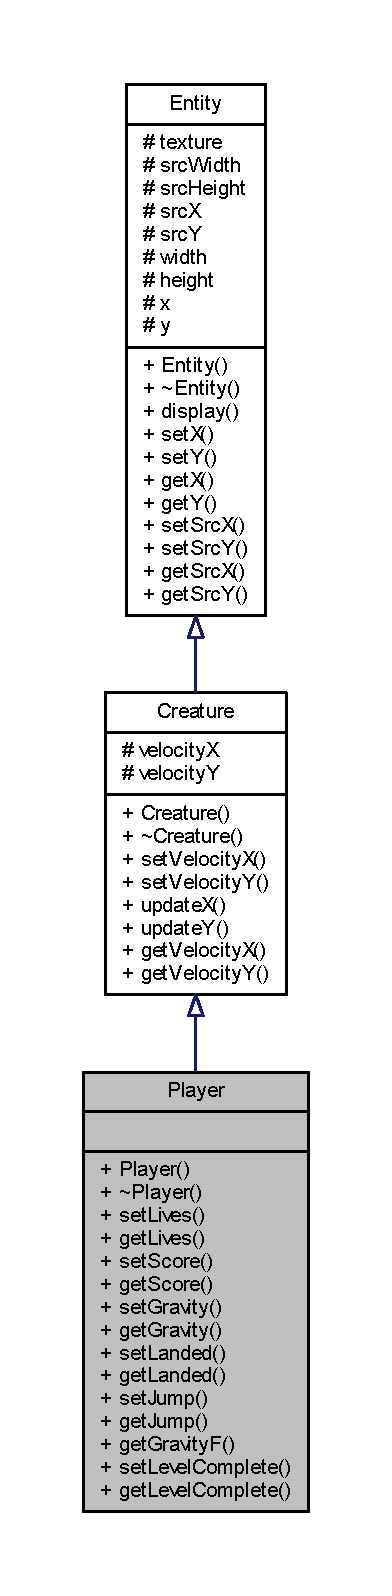
\includegraphics[height=550pt]{class_player__inherit__graph}
\end{center}
\end{figure}


Collaboration diagram for Player\+:
\nopagebreak
\begin{figure}[H]
\begin{center}
\leavevmode
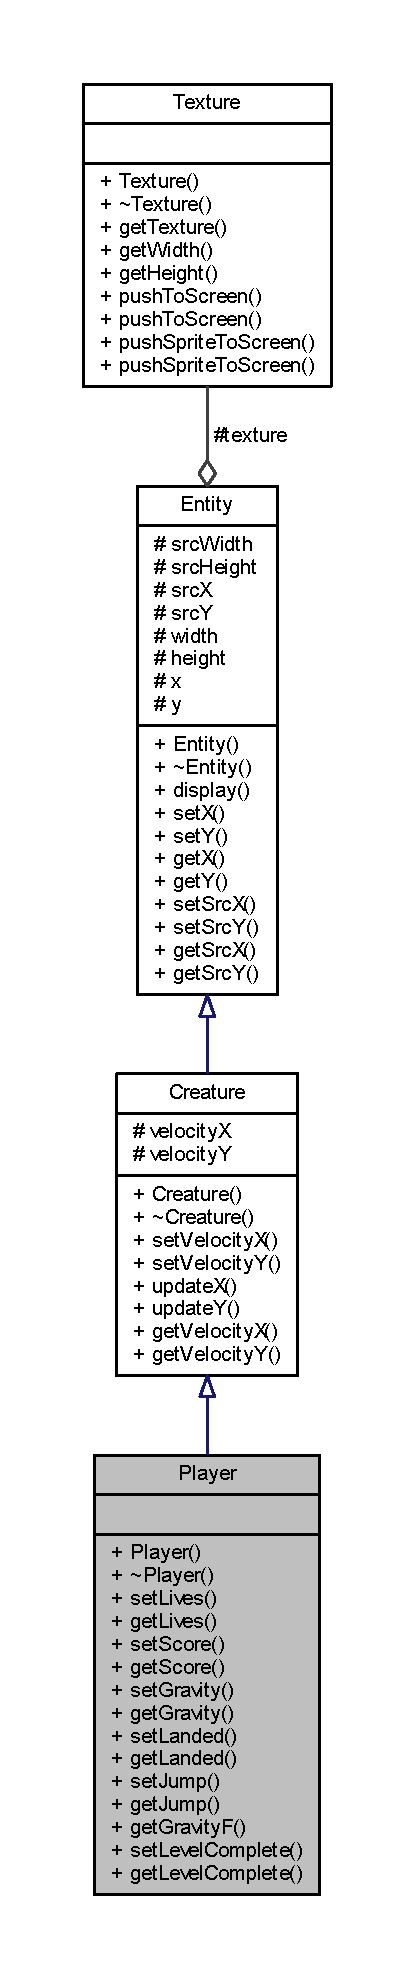
\includegraphics[height=550pt]{class_player__coll__graph}
\end{center}
\end{figure}
\subsection*{Public Member Functions}
\begin{DoxyCompactItemize}
\item 
\hyperlink{class_player_a73d9a9d1017a68d6de107bbfb0a0c486}{Player} (\hyperlink{class_texture}{Texture} $\ast$, float, float, int, int)
\item 
\hyperlink{class_player_a749d2c00e1fe0f5c2746f7505a58c062}{$\sim$\+Player} ()
\item 
void \hyperlink{class_player_a565d4df3c32d00243b1ef16dfd6e5e03}{set\+Lives} (int)
\item 
int \hyperlink{class_player_af56ac33b9b2ebd9f97c8a6f485cf2d47}{get\+Lives} ()
\item 
void \hyperlink{class_player_aa054ea95ca73dd19036d2917b29ab021}{set\+Score} (int)
\item 
int \hyperlink{class_player_a97e5447778ae6c384eedc532dcd8431d}{get\+Score} ()
\item 
void \hyperlink{class_player_a36a300f4f62fae25747c4301a81c5a10}{set\+Gravity} (bool)
\item 
bool \hyperlink{class_player_a7f8e925cef6578c511f0b215f309d814}{get\+Gravity} ()
\item 
void \hyperlink{class_player_a3474c047c1495322742b79a43381bc32}{set\+Landed} (bool)
\item 
bool \hyperlink{class_player_acda5f8d74dcb44e5ebc12003104ec0ef}{get\+Landed} ()
\item 
void \hyperlink{class_player_a282bc0d3c7341a9727bcb16cd902c953}{set\+Jump} (bool)
\item 
bool \hyperlink{class_player_a4760bc30c5c2f45c7a858496a395981f}{get\+Jump} ()
\item 
float \hyperlink{class_player_ae0ae09987c59e99aa451481bf827093c}{get\+Gravity\+F} ()
\item 
void \hyperlink{class_player_a1eb27fc807ef7557979ef23f239a46e5}{set\+Level\+Complete} (bool)
\item 
bool \hyperlink{class_player_a4305af7dca7be99eb5fb8f2002421314}{get\+Level\+Complete} ()
\end{DoxyCompactItemize}
\subsection*{Additional Inherited Members}


\subsection{Detailed Description}
Creates a \hyperlink{class_player}{Player} object that inherits \hyperlink{class_creature}{Creature} which in turn inherits \hyperlink{class_entity}{Entity}. 

\subsection{Constructor \& Destructor Documentation}
\hypertarget{class_player_a73d9a9d1017a68d6de107bbfb0a0c486}{\index{Player@{Player}!Player@{Player}}
\index{Player@{Player}!Player@{Player}}
\subsubsection[{Player}]{\setlength{\rightskip}{0pt plus 5cm}Player\+::\+Player (
\begin{DoxyParamCaption}
\item[{{\bf Texture} $\ast$}]{input\+Texture, }
\item[{float}]{input\+X, }
\item[{float}]{input\+Y, }
\item[{int}]{sprite\+Sheet\+Number\+X, }
\item[{int}]{sprite\+Sheet\+Number\+Y}
\end{DoxyParamCaption}
)}}\label{class_player_a73d9a9d1017a68d6de107bbfb0a0c486}
Constructs a \hyperlink{class_player}{Player} object Constructs the \hyperlink{class_player}{Player} object. 
\begin{DoxyParams}{Parameters}
{\em Texture$\ast$} & a pointer to a \hyperlink{class_texture}{Texture} loaded into memory. \\
\hline
{\em float} & initial x position. \\
\hline
{\em float} & initial y position. \\
\hline
{\em int} & the sprite sheet x number. \\
\hline
{\em int} & the sprite sheet y number. \\
\hline
\end{DoxyParams}
\hypertarget{class_player_a749d2c00e1fe0f5c2746f7505a58c062}{\index{Player@{Player}!````~Player@{$\sim$\+Player}}
\index{````~Player@{$\sim$\+Player}!Player@{Player}}
\subsubsection[{$\sim$\+Player}]{\setlength{\rightskip}{0pt plus 5cm}Player\+::$\sim$\+Player (
\begin{DoxyParamCaption}
{}
\end{DoxyParamCaption}
)}}\label{class_player_a749d2c00e1fe0f5c2746f7505a58c062}
De-\/constructs a \hyperlink{class_player}{Player} object De-\/constructs the \hyperlink{class_player}{Player} object 

\subsection{Member Function Documentation}
\hypertarget{class_player_a7f8e925cef6578c511f0b215f309d814}{\index{Player@{Player}!get\+Gravity@{get\+Gravity}}
\index{get\+Gravity@{get\+Gravity}!Player@{Player}}
\subsubsection[{get\+Gravity}]{\setlength{\rightskip}{0pt plus 5cm}bool Player\+::get\+Gravity (
\begin{DoxyParamCaption}
{}
\end{DoxyParamCaption}
)}}\label{class_player_a7f8e925cef6578c511f0b215f309d814}
Getter \# gravity \begin{DoxyReturn}{Returns}
bool if gravity is acting. 
\end{DoxyReturn}


Here is the caller graph for this function\+:
\nopagebreak
\begin{figure}[H]
\begin{center}
\leavevmode
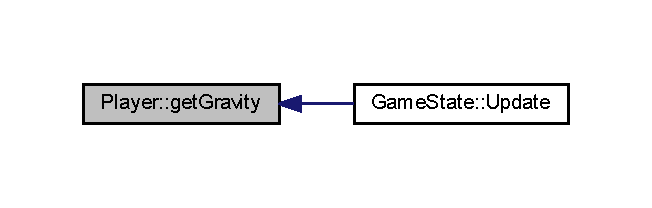
\includegraphics[width=313pt]{class_player_a7f8e925cef6578c511f0b215f309d814_icgraph}
\end{center}
\end{figure}


\hypertarget{class_player_ae0ae09987c59e99aa451481bf827093c}{\index{Player@{Player}!get\+Gravity\+F@{get\+Gravity\+F}}
\index{get\+Gravity\+F@{get\+Gravity\+F}!Player@{Player}}
\subsubsection[{get\+Gravity\+F}]{\setlength{\rightskip}{0pt plus 5cm}float Player\+::get\+Gravity\+F (
\begin{DoxyParamCaption}
{}
\end{DoxyParamCaption}
)}}\label{class_player_ae0ae09987c59e99aa451481bf827093c}
Getter \# gravity\+F \begin{DoxyReturn}{Returns}
float the value of the force gravity. 
\end{DoxyReturn}


Here is the caller graph for this function\+:
\nopagebreak
\begin{figure}[H]
\begin{center}
\leavevmode
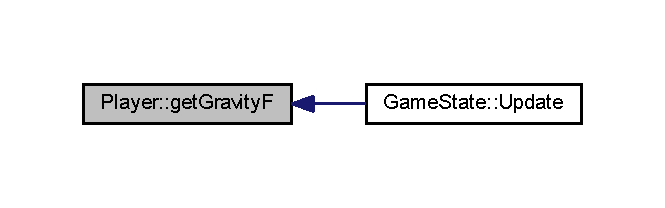
\includegraphics[width=319pt]{class_player_ae0ae09987c59e99aa451481bf827093c_icgraph}
\end{center}
\end{figure}


\hypertarget{class_player_a4760bc30c5c2f45c7a858496a395981f}{\index{Player@{Player}!get\+Jump@{get\+Jump}}
\index{get\+Jump@{get\+Jump}!Player@{Player}}
\subsubsection[{get\+Jump}]{\setlength{\rightskip}{0pt plus 5cm}bool Player\+::get\+Jump (
\begin{DoxyParamCaption}
{}
\end{DoxyParamCaption}
)}}\label{class_player_a4760bc30c5c2f45c7a858496a395981f}
Getter \# jump \begin{DoxyReturn}{Returns}
bool if the \hyperlink{class_player}{Player} is jumping. 
\end{DoxyReturn}
\hypertarget{class_player_acda5f8d74dcb44e5ebc12003104ec0ef}{\index{Player@{Player}!get\+Landed@{get\+Landed}}
\index{get\+Landed@{get\+Landed}!Player@{Player}}
\subsubsection[{get\+Landed}]{\setlength{\rightskip}{0pt plus 5cm}bool Player\+::get\+Landed (
\begin{DoxyParamCaption}
{}
\end{DoxyParamCaption}
)}}\label{class_player_acda5f8d74dcb44e5ebc12003104ec0ef}
Getter \# landed \begin{DoxyReturn}{Returns}
bool if the \hyperlink{class_player}{Player} has landed. 
\end{DoxyReturn}


Here is the caller graph for this function\+:
\nopagebreak
\begin{figure}[H]
\begin{center}
\leavevmode
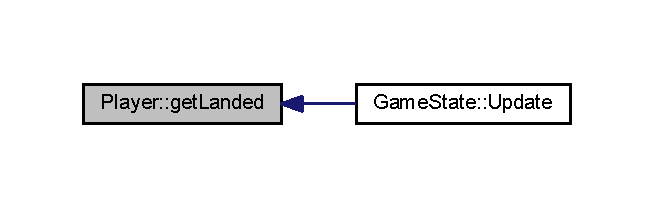
\includegraphics[width=314pt]{class_player_acda5f8d74dcb44e5ebc12003104ec0ef_icgraph}
\end{center}
\end{figure}


\hypertarget{class_player_a4305af7dca7be99eb5fb8f2002421314}{\index{Player@{Player}!get\+Level\+Complete@{get\+Level\+Complete}}
\index{get\+Level\+Complete@{get\+Level\+Complete}!Player@{Player}}
\subsubsection[{get\+Level\+Complete}]{\setlength{\rightskip}{0pt plus 5cm}bool Player\+::get\+Level\+Complete (
\begin{DoxyParamCaption}
{}
\end{DoxyParamCaption}
)}}\label{class_player_a4305af7dca7be99eb5fb8f2002421314}
Getter \# level complete \begin{DoxyReturn}{Returns}
bool if the \hyperlink{class_player}{Player} has finished the level. 
\end{DoxyReturn}


Here is the caller graph for this function\+:
\nopagebreak
\begin{figure}[H]
\begin{center}
\leavevmode
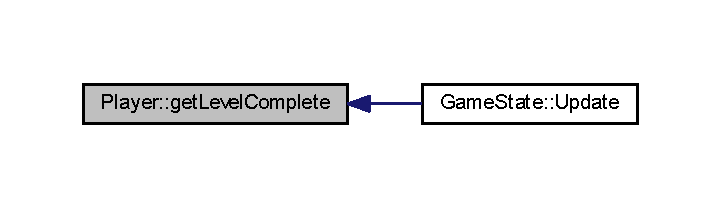
\includegraphics[width=346pt]{class_player_a4305af7dca7be99eb5fb8f2002421314_icgraph}
\end{center}
\end{figure}


\hypertarget{class_player_af56ac33b9b2ebd9f97c8a6f485cf2d47}{\index{Player@{Player}!get\+Lives@{get\+Lives}}
\index{get\+Lives@{get\+Lives}!Player@{Player}}
\subsubsection[{get\+Lives}]{\setlength{\rightskip}{0pt plus 5cm}int Player\+::get\+Lives (
\begin{DoxyParamCaption}
{}
\end{DoxyParamCaption}
)}}\label{class_player_af56ac33b9b2ebd9f97c8a6f485cf2d47}
Getter \# lives \begin{DoxyReturn}{Returns}
int the number of lives the \hyperlink{class_player}{Player} has. 
\end{DoxyReturn}


Here is the caller graph for this function\+:
\nopagebreak
\begin{figure}[H]
\begin{center}
\leavevmode
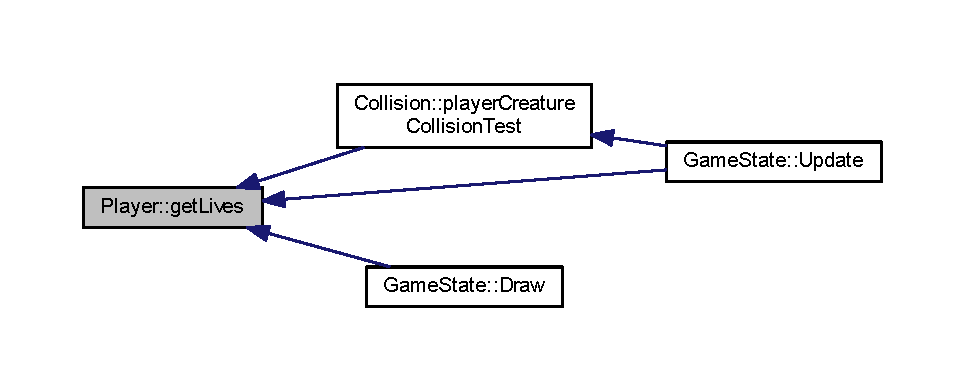
\includegraphics[width=350pt]{class_player_af56ac33b9b2ebd9f97c8a6f485cf2d47_icgraph}
\end{center}
\end{figure}


\hypertarget{class_player_a97e5447778ae6c384eedc532dcd8431d}{\index{Player@{Player}!get\+Score@{get\+Score}}
\index{get\+Score@{get\+Score}!Player@{Player}}
\subsubsection[{get\+Score}]{\setlength{\rightskip}{0pt plus 5cm}int Player\+::get\+Score (
\begin{DoxyParamCaption}
{}
\end{DoxyParamCaption}
)}}\label{class_player_a97e5447778ae6c384eedc532dcd8431d}
Getter \# score \begin{DoxyReturn}{Returns}
int the score the \hyperlink{class_player}{Player} has. 
\end{DoxyReturn}


Here is the caller graph for this function\+:
\nopagebreak
\begin{figure}[H]
\begin{center}
\leavevmode
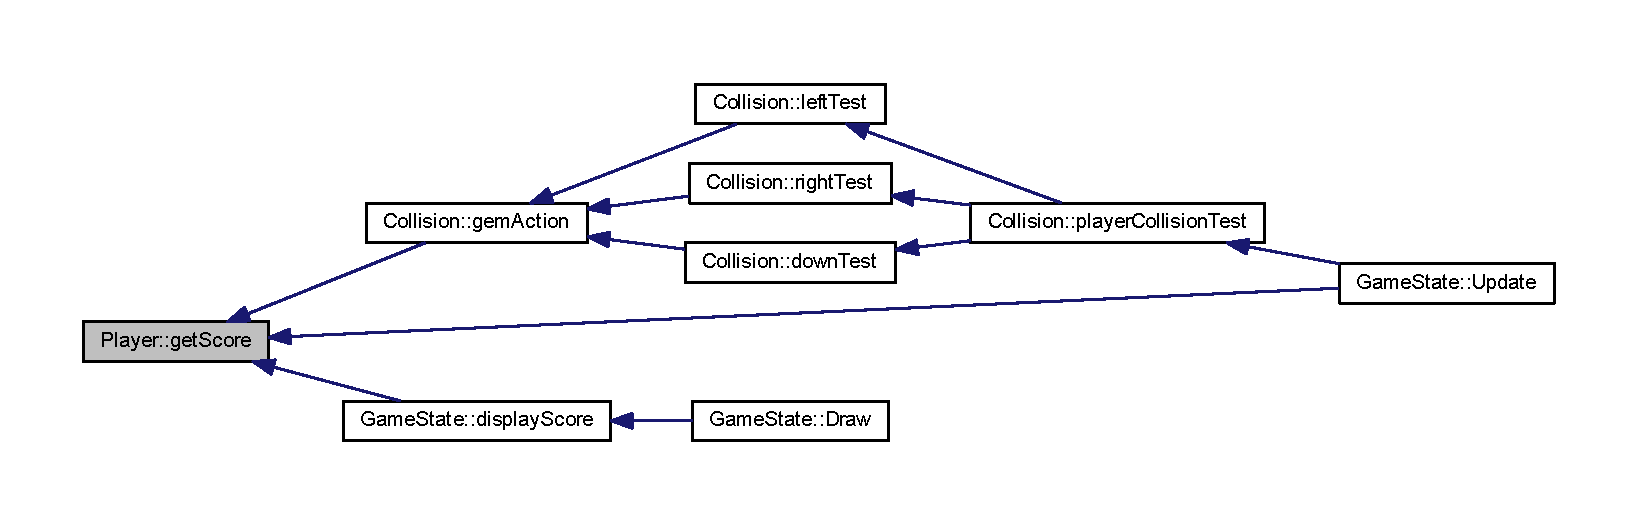
\includegraphics[width=350pt]{class_player_a97e5447778ae6c384eedc532dcd8431d_icgraph}
\end{center}
\end{figure}


\hypertarget{class_player_a36a300f4f62fae25747c4301a81c5a10}{\index{Player@{Player}!set\+Gravity@{set\+Gravity}}
\index{set\+Gravity@{set\+Gravity}!Player@{Player}}
\subsubsection[{set\+Gravity}]{\setlength{\rightskip}{0pt plus 5cm}void Player\+::set\+Gravity (
\begin{DoxyParamCaption}
\item[{bool}]{input\+Gravity}
\end{DoxyParamCaption}
)}}\label{class_player_a36a300f4f62fae25747c4301a81c5a10}
Setter \# gravity Sets if gravity is acting on not. 
\begin{DoxyParams}{Parameters}
{\em bool} & if gravity is acting. \\
\hline
\end{DoxyParams}


Here is the caller graph for this function\+:
\nopagebreak
\begin{figure}[H]
\begin{center}
\leavevmode
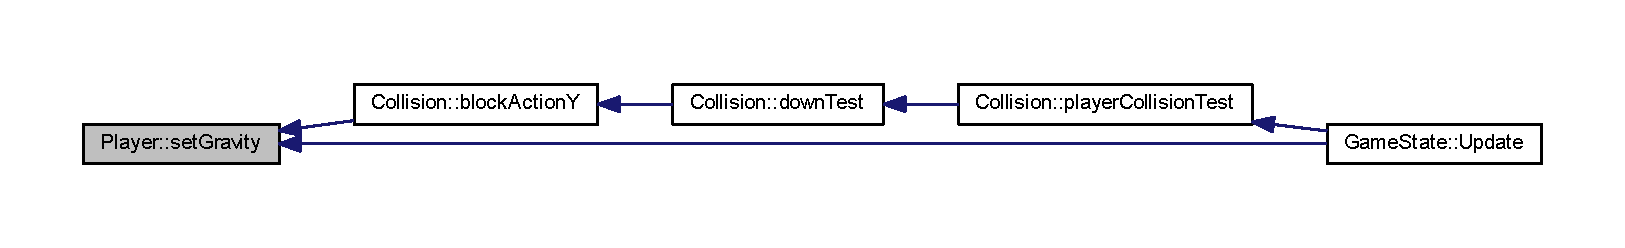
\includegraphics[width=350pt]{class_player_a36a300f4f62fae25747c4301a81c5a10_icgraph}
\end{center}
\end{figure}


\hypertarget{class_player_a282bc0d3c7341a9727bcb16cd902c953}{\index{Player@{Player}!set\+Jump@{set\+Jump}}
\index{set\+Jump@{set\+Jump}!Player@{Player}}
\subsubsection[{set\+Jump}]{\setlength{\rightskip}{0pt plus 5cm}void Player\+::set\+Jump (
\begin{DoxyParamCaption}
\item[{bool}]{input\+Jump}
\end{DoxyParamCaption}
)}}\label{class_player_a282bc0d3c7341a9727bcb16cd902c953}
Setter \# jump Sets if the \hyperlink{class_player}{Player} is jumping. 
\begin{DoxyParams}{Parameters}
{\em bool} & if the \hyperlink{class_player}{Player} is jumping. \\
\hline
\end{DoxyParams}
\hypertarget{class_player_a3474c047c1495322742b79a43381bc32}{\index{Player@{Player}!set\+Landed@{set\+Landed}}
\index{set\+Landed@{set\+Landed}!Player@{Player}}
\subsubsection[{set\+Landed}]{\setlength{\rightskip}{0pt plus 5cm}void Player\+::set\+Landed (
\begin{DoxyParamCaption}
\item[{bool}]{input\+Landing}
\end{DoxyParamCaption}
)}}\label{class_player_a3474c047c1495322742b79a43381bc32}
Setter \# landed Sets if the \hyperlink{class_player}{Player} has landed. 
\begin{DoxyParams}{Parameters}
{\em bool} & if the \hyperlink{class_player}{Player} has landed. \\
\hline
\end{DoxyParams}


Here is the caller graph for this function\+:
\nopagebreak
\begin{figure}[H]
\begin{center}
\leavevmode
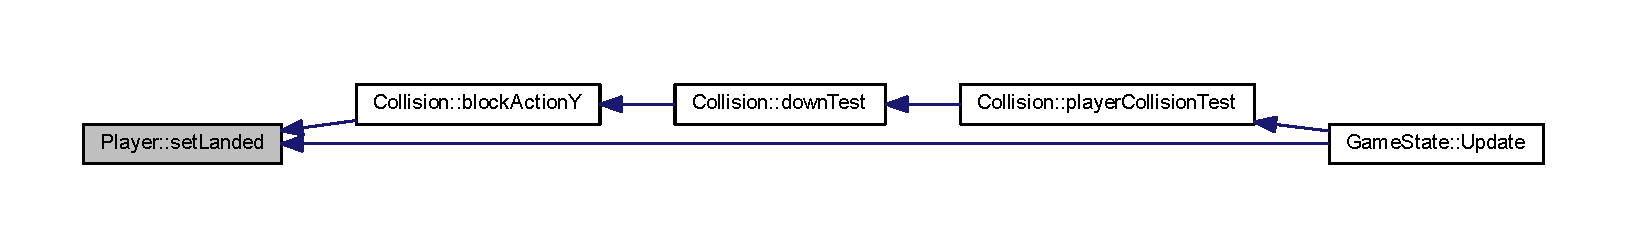
\includegraphics[width=350pt]{class_player_a3474c047c1495322742b79a43381bc32_icgraph}
\end{center}
\end{figure}


\hypertarget{class_player_a1eb27fc807ef7557979ef23f239a46e5}{\index{Player@{Player}!set\+Level\+Complete@{set\+Level\+Complete}}
\index{set\+Level\+Complete@{set\+Level\+Complete}!Player@{Player}}
\subsubsection[{set\+Level\+Complete}]{\setlength{\rightskip}{0pt plus 5cm}void Player\+::set\+Level\+Complete (
\begin{DoxyParamCaption}
\item[{bool}]{input\+Level\+Complete}
\end{DoxyParamCaption}
)}}\label{class_player_a1eb27fc807ef7557979ef23f239a46e5}
Setter \# level complete Sets if the \hyperlink{class_player}{Player} has finished the level. 
\begin{DoxyParams}{Parameters}
{\em bool} & if the \hyperlink{class_player}{Player} has finished the level. \\
\hline
\end{DoxyParams}


Here is the caller graph for this function\+:
\nopagebreak
\begin{figure}[H]
\begin{center}
\leavevmode
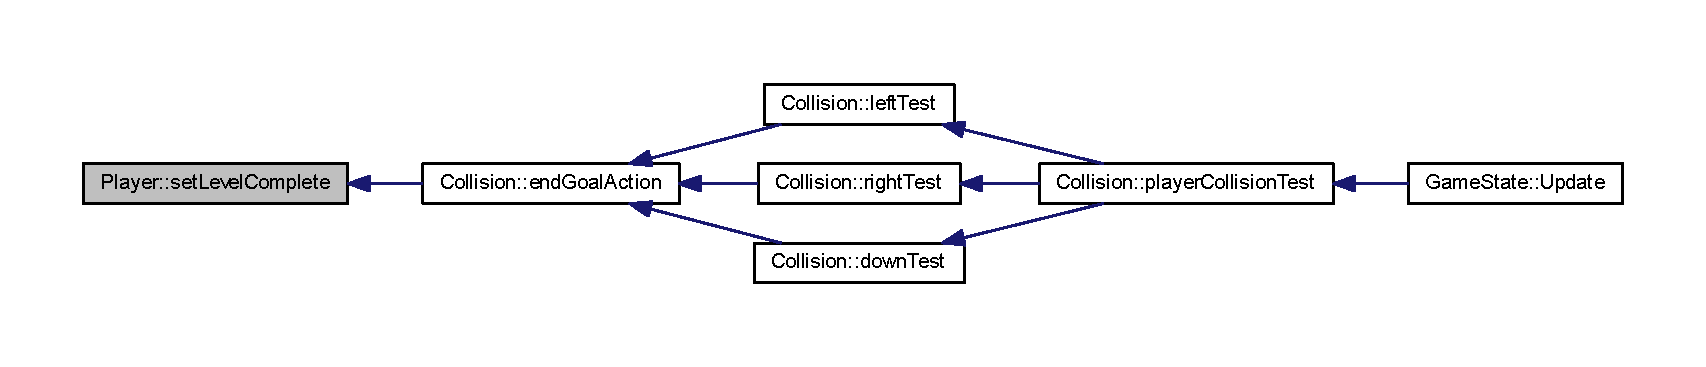
\includegraphics[width=350pt]{class_player_a1eb27fc807ef7557979ef23f239a46e5_icgraph}
\end{center}
\end{figure}


\hypertarget{class_player_a565d4df3c32d00243b1ef16dfd6e5e03}{\index{Player@{Player}!set\+Lives@{set\+Lives}}
\index{set\+Lives@{set\+Lives}!Player@{Player}}
\subsubsection[{set\+Lives}]{\setlength{\rightskip}{0pt plus 5cm}void Player\+::set\+Lives (
\begin{DoxyParamCaption}
\item[{int}]{input\+Lives}
\end{DoxyParamCaption}
)}}\label{class_player_a565d4df3c32d00243b1ef16dfd6e5e03}
Setter \# lives Sets the number of lives of the \hyperlink{class_player}{Player} object to the inputed number. 
\begin{DoxyParams}{Parameters}
{\em int} & the inputed number of lives \\
\hline
\end{DoxyParams}


Here is the caller graph for this function\+:
\nopagebreak
\begin{figure}[H]
\begin{center}
\leavevmode
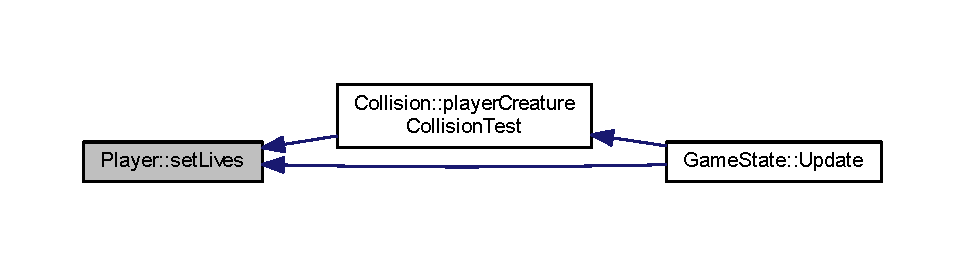
\includegraphics[width=350pt]{class_player_a565d4df3c32d00243b1ef16dfd6e5e03_icgraph}
\end{center}
\end{figure}


\hypertarget{class_player_aa054ea95ca73dd19036d2917b29ab021}{\index{Player@{Player}!set\+Score@{set\+Score}}
\index{set\+Score@{set\+Score}!Player@{Player}}
\subsubsection[{set\+Score}]{\setlength{\rightskip}{0pt plus 5cm}void Player\+::set\+Score (
\begin{DoxyParamCaption}
\item[{int}]{input\+Score}
\end{DoxyParamCaption}
)}}\label{class_player_aa054ea95ca73dd19036d2917b29ab021}
Setter \# score Sets the score of the \hyperlink{class_player}{Player} object to the inputed number. 
\begin{DoxyParams}{Parameters}
{\em int} & the inputed score \\
\hline
\end{DoxyParams}


Here is the caller graph for this function\+:
\nopagebreak
\begin{figure}[H]
\begin{center}
\leavevmode
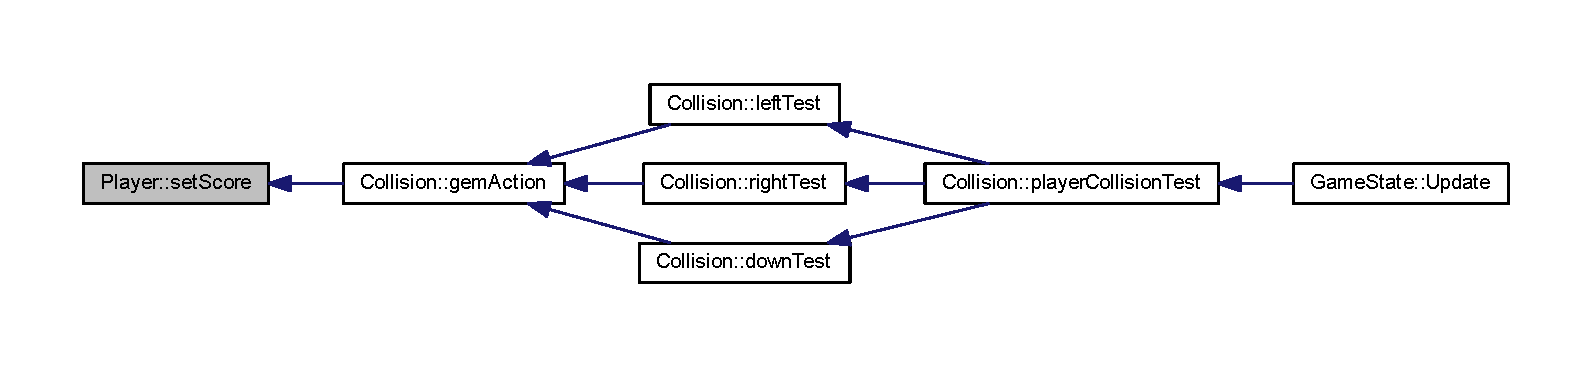
\includegraphics[width=350pt]{class_player_aa054ea95ca73dd19036d2917b29ab021_icgraph}
\end{center}
\end{figure}




The documentation for this class was generated from the following files\+:\begin{DoxyCompactItemize}
\item 
P\+G\+G\+Assignment1\+S\+D\+L/player.\+h\item 
P\+G\+G\+Assignment1\+S\+D\+L/player.\+cpp\end{DoxyCompactItemize}

\hypertarget{class_state}{\section{State Class Reference}
\label{class_state}\index{State@{State}}
}


Creates a \hyperlink{class_state}{State} object. Creates a \hyperlink{class_state}{State} object to be inherited. Made using information from \href{http://blog.nuclex-games.com/tutorials/cxx/game-state-management/}{\tt http\+://blog.\+nuclex-\/games.\+com/tutorials/cxx/game-\/state-\/management/} and Peter Allen.  




{\ttfamily \#include $<$state.\+h$>$}



Inheritance diagram for State\+:
\nopagebreak
\begin{figure}[H]
\begin{center}
\leavevmode
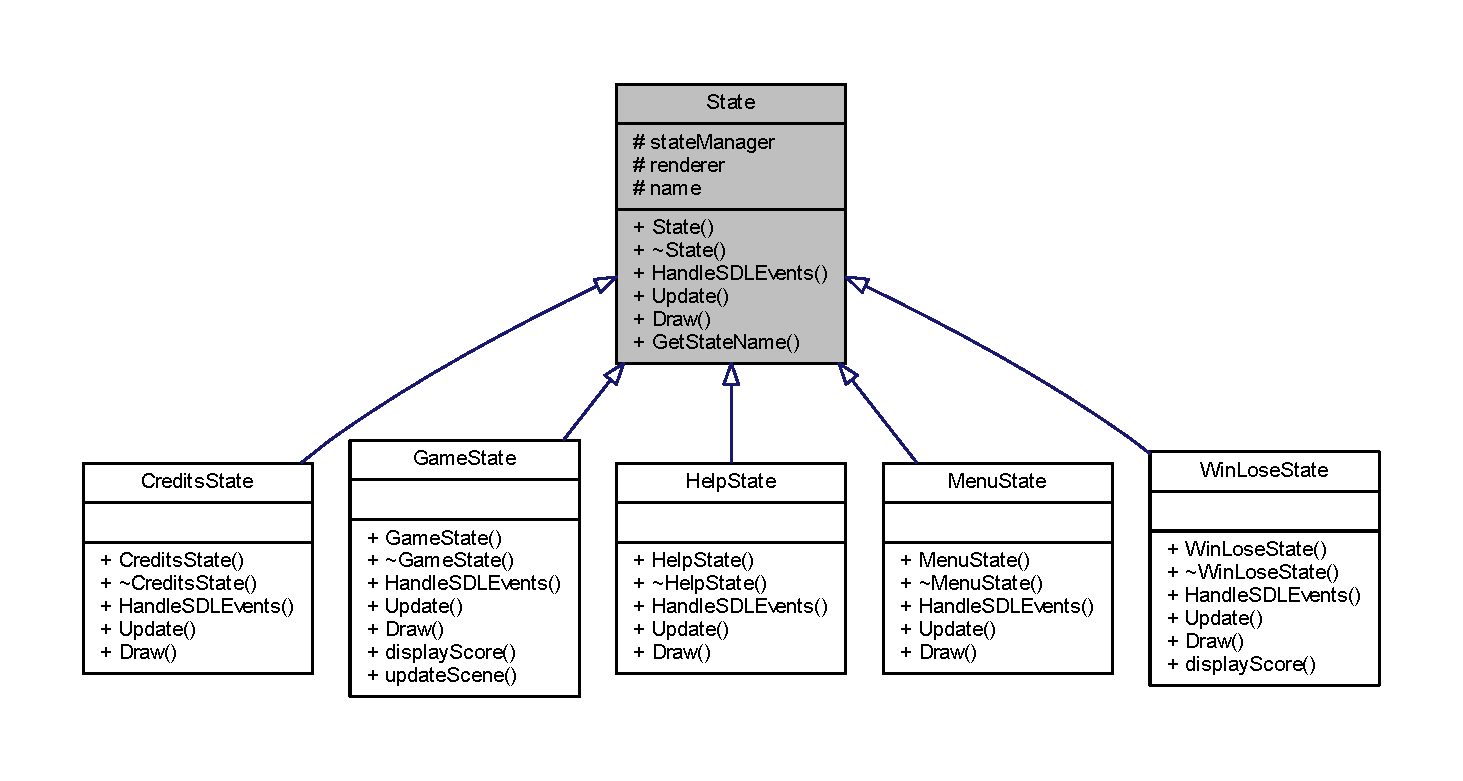
\includegraphics[width=350pt]{class_state__inherit__graph}
\end{center}
\end{figure}


Collaboration diagram for State\+:
\nopagebreak
\begin{figure}[H]
\begin{center}
\leavevmode
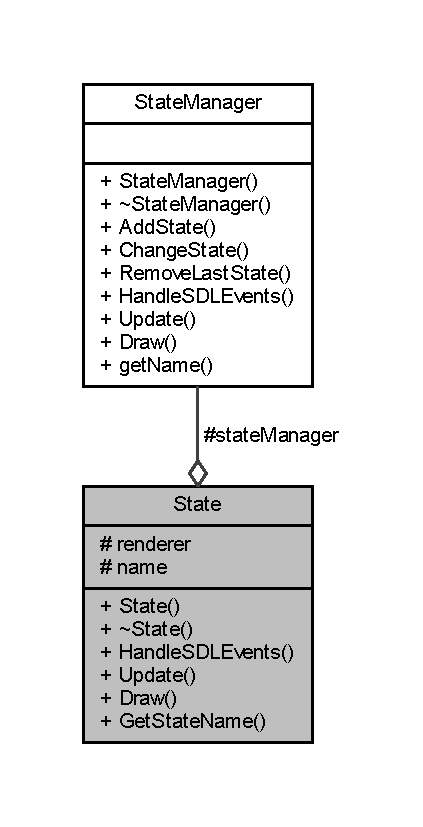
\includegraphics[width=203pt]{class_state__coll__graph}
\end{center}
\end{figure}
\subsection*{Public Member Functions}
\begin{DoxyCompactItemize}
\item 
\hyperlink{class_state_abd80317215e3d5a83becc409050dd22f}{State} (\hyperlink{class_state_manager}{State\+Manager} $\ast$, S\+D\+L\+\_\+\+Renderer $\ast$)
\item 
virtual \hyperlink{class_state_afab438d92b90dc18d194dbd9c9c8bab3}{$\sim$\+State} ()
\item 
virtual bool \hyperlink{class_state_a648d9182cab9aeb914ef778f94e2b437}{Handle\+S\+D\+L\+Events} ()=0
\item 
virtual void \hyperlink{class_state_a770f40188fdfc64bc95a5166fef12e02}{Update} (float delta\+Time)=0
\item 
virtual void \hyperlink{class_state_a8b0cdb0e7450a9bb3580a33dfbe4d981}{Draw} ()=0
\item 
std\+::string \hyperlink{class_state_ab7a5d1c1837b4b44b3563897777fcb26}{Get\+State\+Name} ()
\end{DoxyCompactItemize}
\subsection*{Protected Attributes}
\begin{DoxyCompactItemize}
\item 
\hypertarget{class_state_a78388f59b0a570faa4b7ea640fea668e}{\hyperlink{class_state_manager}{State\+Manager} $\ast$ {\bfseries state\+Manager}}\label{class_state_a78388f59b0a570faa4b7ea640fea668e}

\item 
\hypertarget{class_state_ad79f979055823ec66fb7919e90ddd5c9}{S\+D\+L\+\_\+\+Renderer $\ast$ {\bfseries renderer}}\label{class_state_ad79f979055823ec66fb7919e90ddd5c9}

\item 
\hypertarget{class_state_ad57f19fd0a86f129840d8739253d2c72}{std\+::string {\bfseries name}}\label{class_state_ad57f19fd0a86f129840d8739253d2c72}

\end{DoxyCompactItemize}


\subsection{Detailed Description}
Creates a \hyperlink{class_state}{State} object. Creates a \hyperlink{class_state}{State} object to be inherited. Made using information from \href{http://blog.nuclex-games.com/tutorials/cxx/game-state-management/}{\tt http\+://blog.\+nuclex-\/games.\+com/tutorials/cxx/game-\/state-\/management/} and Peter Allen. 

\subsection{Constructor \& Destructor Documentation}
\hypertarget{class_state_abd80317215e3d5a83becc409050dd22f}{\index{State@{State}!State@{State}}
\index{State@{State}!State@{State}}
\subsubsection[{State}]{\setlength{\rightskip}{0pt plus 5cm}State\+::\+State (
\begin{DoxyParamCaption}
\item[{{\bf State\+Manager} $\ast$}]{in\+State\+Manager, }
\item[{S\+D\+L\+\_\+\+Renderer $\ast$}]{in\+Renderer}
\end{DoxyParamCaption}
)}}\label{class_state_abd80317215e3d5a83becc409050dd22f}
Constructs a \hyperlink{class_state}{State} object Constructs a \hyperlink{class_state}{State} object 
\begin{DoxyParams}{Parameters}
{\em \hyperlink{class_state_manager}{State\+Manager}} & $\ast$ a pointer to the \hyperlink{class_state_manager}{State\+Manager} \\
\hline
{\em S\+D\+L\+\_\+\+Renderer} & $\ast$ a pointer to the renderer in use. \\
\hline
\end{DoxyParams}
\hypertarget{class_state_afab438d92b90dc18d194dbd9c9c8bab3}{\index{State@{State}!````~State@{$\sim$\+State}}
\index{````~State@{$\sim$\+State}!State@{State}}
\subsubsection[{$\sim$\+State}]{\setlength{\rightskip}{0pt plus 5cm}State\+::$\sim$\+State (
\begin{DoxyParamCaption}
{}
\end{DoxyParamCaption}
)\hspace{0.3cm}{\ttfamily [virtual]}}}\label{class_state_afab438d92b90dc18d194dbd9c9c8bab3}
A virtual destructor for the \hyperlink{class_state}{State} object A virtual destructor for the \hyperlink{class_state}{State} object 

\subsection{Member Function Documentation}
\hypertarget{class_state_a8b0cdb0e7450a9bb3580a33dfbe4d981}{\index{State@{State}!Draw@{Draw}}
\index{Draw@{Draw}!State@{State}}
\subsubsection[{Draw}]{\setlength{\rightskip}{0pt plus 5cm}virtual void State\+::\+Draw (
\begin{DoxyParamCaption}
{}
\end{DoxyParamCaption}
)\hspace{0.3cm}{\ttfamily [pure virtual]}}}\label{class_state_a8b0cdb0e7450a9bb3580a33dfbe4d981}
A virtual function to draw to the screen A virtual function to draw to the screen using the renderer 

Implemented in \hyperlink{class_game_state_ab9330b36c7c74d733c2739c025285c64}{Game\+State}, \hyperlink{class_menu_state_a0fc92c6a39ef316552f1308c188871c6}{Menu\+State}, \hyperlink{class_win_lose_state_a862a5bb9422480b36671acb21cc987ba}{Win\+Lose\+State}, \hyperlink{class_credits_state_a4027aad0c48b505a74faef47470622a1}{Credits\+State}, and \hyperlink{class_help_state_a281d12605303cc444e600b214a8d2161}{Help\+State}.

\hypertarget{class_state_ab7a5d1c1837b4b44b3563897777fcb26}{\index{State@{State}!Get\+State\+Name@{Get\+State\+Name}}
\index{Get\+State\+Name@{Get\+State\+Name}!State@{State}}
\subsubsection[{Get\+State\+Name}]{\setlength{\rightskip}{0pt plus 5cm}std\+::string State\+::\+Get\+State\+Name (
\begin{DoxyParamCaption}
{}
\end{DoxyParamCaption}
)}}\label{class_state_ab7a5d1c1837b4b44b3563897777fcb26}
Getter \# \hyperlink{class_state}{State} name \begin{DoxyReturn}{Returns}
the name of the \hyperlink{class_state}{State}. 
\end{DoxyReturn}
\hypertarget{class_state_a648d9182cab9aeb914ef778f94e2b437}{\index{State@{State}!Handle\+S\+D\+L\+Events@{Handle\+S\+D\+L\+Events}}
\index{Handle\+S\+D\+L\+Events@{Handle\+S\+D\+L\+Events}!State@{State}}
\subsubsection[{Handle\+S\+D\+L\+Events}]{\setlength{\rightskip}{0pt plus 5cm}virtual bool State\+::\+Handle\+S\+D\+L\+Events (
\begin{DoxyParamCaption}
{}
\end{DoxyParamCaption}
)\hspace{0.3cm}{\ttfamily [pure virtual]}}}\label{class_state_a648d9182cab9aeb914ef778f94e2b437}
A virtual function to handle the S\+D\+L events A virtual function to handle the S\+D\+L events for use with the \hyperlink{class_state}{State} \begin{DoxyReturn}{Returns}
bool if false then quit \hyperlink{class_state}{State} 
\end{DoxyReturn}


Implemented in \hyperlink{class_game_state_a5e2467775e9a941d482e0489295c363d}{Game\+State}, \hyperlink{class_menu_state_abab3b8017d47c6d6134cbdfb8e0c7580}{Menu\+State}, \hyperlink{class_win_lose_state_ada8c41baa8011df1aeae4b7b0d9b00f8}{Win\+Lose\+State}, \hyperlink{class_credits_state_a952d9a50d529f1ba4d883b4a37f558d4}{Credits\+State}, and \hyperlink{class_help_state_a7149e10e0129b66a68290d259bce3015}{Help\+State}.

\hypertarget{class_state_a770f40188fdfc64bc95a5166fef12e02}{\index{State@{State}!Update@{Update}}
\index{Update@{Update}!State@{State}}
\subsubsection[{Update}]{\setlength{\rightskip}{0pt plus 5cm}virtual void State\+::\+Update (
\begin{DoxyParamCaption}
\item[{float}]{delta\+Time}
\end{DoxyParamCaption}
)\hspace{0.3cm}{\ttfamily [pure virtual]}}}\label{class_state_a770f40188fdfc64bc95a5166fef12e02}
A virtual function to update the \hyperlink{class_state}{State} A virtual function to update the \hyperlink{class_state}{State} to allow the \hyperlink{class_state}{State} to run 
\begin{DoxyParams}{Parameters}
{\em float} & the delta time \\
\hline
\end{DoxyParams}


Implemented in \hyperlink{class_game_state_a2ea32b0cd5f747ef6223d182f415a6c4}{Game\+State}, \hyperlink{class_menu_state_a2ee9793bd50c42d8c7ce4cab62fbeba6}{Menu\+State}, \hyperlink{class_win_lose_state_a98e675ce31aa41ad95ba36fd9e77dde6}{Win\+Lose\+State}, \hyperlink{class_credits_state_ab9ad90f4b1c6ddab6ff1234a92c9aec1}{Credits\+State}, and \hyperlink{class_help_state_ac9a45859141cae970629aac1e7a69184}{Help\+State}.



The documentation for this class was generated from the following files\+:\begin{DoxyCompactItemize}
\item 
P\+G\+G\+Assignment1\+S\+D\+L/state.\+h\item 
P\+G\+G\+Assignment1\+S\+D\+L/state.\+cpp\end{DoxyCompactItemize}

\hypertarget{class_state_manager}{\section{State\+Manager Class Reference}
\label{class_state_manager}\index{State\+Manager@{State\+Manager}}
}


Creates a \hyperlink{class_state}{State} manager object. Creates a \hyperlink{class_state}{State} manager object to be inherited. Made using information from \href{http://blog.nuclex-games.com/tutorials/cxx/game-state-management/}{\tt http\+://blog.\+nuclex-\/games.\+com/tutorials/cxx/game-\/state-\/management/} and Peter Allen.  




{\ttfamily \#include $<$state\+Manager.\+h$>$}

\subsection*{Public Member Functions}
\begin{DoxyCompactItemize}
\item 
\hyperlink{class_state_manager_a3e2be96d935eb56813b096a885d58587}{State\+Manager} ()
\item 
\hyperlink{class_state_manager_a05a43504a033f1befad5c5118249ec6f}{$\sim$\+State\+Manager} ()
\item 
void \hyperlink{class_state_manager_aa925e9a15bba3cc4b262a08c8024ea3b}{Add\+State} (\hyperlink{class_state}{State} $\ast$)
\item 
void \hyperlink{class_state_manager_a8c14290973150a37afdf365d00ffcbba}{Change\+State} (\hyperlink{class_state}{State} $\ast$)
\item 
void \hyperlink{class_state_manager_ac782f24f5c02c27169bc2b3bf7aa3d41}{Remove\+Last\+State} ()
\item 
bool \hyperlink{class_state_manager_a10042662c52179ea1ad85051562ca4bf}{Handle\+S\+D\+L\+Events} ()
\item 
void \hyperlink{class_state_manager_a0b430dbaff295c0f96d365da8113fd31}{Update} (float delta\+Time)
\item 
void \hyperlink{class_state_manager_a2827f9e10336c53c7957ed5c09cb2a49}{Draw} ()
\item 
std\+::string \hyperlink{class_state_manager_afc67a8f9404b7c92237a654630eb7516}{get\+Name} ()
\end{DoxyCompactItemize}


\subsection{Detailed Description}
Creates a \hyperlink{class_state}{State} manager object. Creates a \hyperlink{class_state}{State} manager object to be inherited. Made using information from \href{http://blog.nuclex-games.com/tutorials/cxx/game-state-management/}{\tt http\+://blog.\+nuclex-\/games.\+com/tutorials/cxx/game-\/state-\/management/} and Peter Allen. 

\subsection{Constructor \& Destructor Documentation}
\hypertarget{class_state_manager_a3e2be96d935eb56813b096a885d58587}{\index{State\+Manager@{State\+Manager}!State\+Manager@{State\+Manager}}
\index{State\+Manager@{State\+Manager}!State\+Manager@{State\+Manager}}
\subsubsection[{State\+Manager}]{\setlength{\rightskip}{0pt plus 5cm}State\+Manager\+::\+State\+Manager (
\begin{DoxyParamCaption}
{}
\end{DoxyParamCaption}
)}}\label{class_state_manager_a3e2be96d935eb56813b096a885d58587}
Constructs a \hyperlink{class_state_manager}{State\+Manager} object Constructs a \hyperlink{class_state_manager}{State\+Manager} object \hypertarget{class_state_manager_a05a43504a033f1befad5c5118249ec6f}{\index{State\+Manager@{State\+Manager}!````~State\+Manager@{$\sim$\+State\+Manager}}
\index{````~State\+Manager@{$\sim$\+State\+Manager}!State\+Manager@{State\+Manager}}
\subsubsection[{$\sim$\+State\+Manager}]{\setlength{\rightskip}{0pt plus 5cm}State\+Manager\+::$\sim$\+State\+Manager (
\begin{DoxyParamCaption}
{}
\end{DoxyParamCaption}
)}}\label{class_state_manager_a05a43504a033f1befad5c5118249ec6f}
De-\/constructs a \hyperlink{class_state_manager}{State\+Manager} object De-\/constructs the \hyperlink{class_state_manager}{State\+Manager} object 

\subsection{Member Function Documentation}
\hypertarget{class_state_manager_aa925e9a15bba3cc4b262a08c8024ea3b}{\index{State\+Manager@{State\+Manager}!Add\+State@{Add\+State}}
\index{Add\+State@{Add\+State}!State\+Manager@{State\+Manager}}
\subsubsection[{Add\+State}]{\setlength{\rightskip}{0pt plus 5cm}void State\+Manager\+::\+Add\+State (
\begin{DoxyParamCaption}
\item[{{\bf State} $\ast$}]{state}
\end{DoxyParamCaption}
)}}\label{class_state_manager_aa925e9a15bba3cc4b262a08c8024ea3b}
Adds a new state Adds a new state to the current stack of states 
\begin{DoxyParams}{Parameters}
{\em \hyperlink{class_state}{State}} & $\ast$ a pointer to the \hyperlink{class_state}{State} in use \\
\hline
\end{DoxyParams}
\hypertarget{class_state_manager_a8c14290973150a37afdf365d00ffcbba}{\index{State\+Manager@{State\+Manager}!Change\+State@{Change\+State}}
\index{Change\+State@{Change\+State}!State\+Manager@{State\+Manager}}
\subsubsection[{Change\+State}]{\setlength{\rightskip}{0pt plus 5cm}void State\+Manager\+::\+Change\+State (
\begin{DoxyParamCaption}
\item[{{\bf State} $\ast$}]{state}
\end{DoxyParamCaption}
)}}\label{class_state_manager_a8c14290973150a37afdf365d00ffcbba}
Changes to a new \hyperlink{class_state}{State} Changes the current \hyperlink{class_state}{State} to a new \hyperlink{class_state}{State} 
\begin{DoxyParams}{Parameters}
{\em \hyperlink{class_state}{State}} & $\ast$ a pointer to the \hyperlink{class_state}{State} in use \\
\hline
\end{DoxyParams}
\hypertarget{class_state_manager_a2827f9e10336c53c7957ed5c09cb2a49}{\index{State\+Manager@{State\+Manager}!Draw@{Draw}}
\index{Draw@{Draw}!State\+Manager@{State\+Manager}}
\subsubsection[{Draw}]{\setlength{\rightskip}{0pt plus 5cm}void State\+Manager\+::\+Draw (
\begin{DoxyParamCaption}
{}
\end{DoxyParamCaption}
)}}\label{class_state_manager_a2827f9e10336c53c7957ed5c09cb2a49}
Draws the current \hyperlink{class_state}{State} The draw function that will allow the equivalent draw function to run in the current \hyperlink{class_state}{State} \hypertarget{class_state_manager_afc67a8f9404b7c92237a654630eb7516}{\index{State\+Manager@{State\+Manager}!get\+Name@{get\+Name}}
\index{get\+Name@{get\+Name}!State\+Manager@{State\+Manager}}
\subsubsection[{get\+Name}]{\setlength{\rightskip}{0pt plus 5cm}std\+::string State\+Manager\+::get\+Name (
\begin{DoxyParamCaption}
{}
\end{DoxyParamCaption}
)}}\label{class_state_manager_afc67a8f9404b7c92237a654630eb7516}
getter \# the name of the current \hyperlink{class_state}{State} gets the name of the current \hyperlink{class_state}{State} \begin{DoxyReturn}{Returns}
std\+::string the name of the state 
\end{DoxyReturn}
\hypertarget{class_state_manager_a10042662c52179ea1ad85051562ca4bf}{\index{State\+Manager@{State\+Manager}!Handle\+S\+D\+L\+Events@{Handle\+S\+D\+L\+Events}}
\index{Handle\+S\+D\+L\+Events@{Handle\+S\+D\+L\+Events}!State\+Manager@{State\+Manager}}
\subsubsection[{Handle\+S\+D\+L\+Events}]{\setlength{\rightskip}{0pt plus 5cm}bool State\+Manager\+::\+Handle\+S\+D\+L\+Events (
\begin{DoxyParamCaption}
{}
\end{DoxyParamCaption}
)}}\label{class_state_manager_a10042662c52179ea1ad85051562ca4bf}
Handles the S\+D\+L events The S\+D\+L event handler function that will allow the equivalent S\+D\+L event handler function to run in the current \hyperlink{class_state}{State} \begin{DoxyReturn}{Returns}
bool if false then quit the application 
\end{DoxyReturn}
\hypertarget{class_state_manager_ac782f24f5c02c27169bc2b3bf7aa3d41}{\index{State\+Manager@{State\+Manager}!Remove\+Last\+State@{Remove\+Last\+State}}
\index{Remove\+Last\+State@{Remove\+Last\+State}!State\+Manager@{State\+Manager}}
\subsubsection[{Remove\+Last\+State}]{\setlength{\rightskip}{0pt plus 5cm}void State\+Manager\+::\+Remove\+Last\+State (
\begin{DoxyParamCaption}
{}
\end{DoxyParamCaption}
)}}\label{class_state_manager_ac782f24f5c02c27169bc2b3bf7aa3d41}
Removes the last \hyperlink{class_state}{State} from the vector Removes the last \hyperlink{class_state}{State} from the vector \hypertarget{class_state_manager_a0b430dbaff295c0f96d365da8113fd31}{\index{State\+Manager@{State\+Manager}!Update@{Update}}
\index{Update@{Update}!State\+Manager@{State\+Manager}}
\subsubsection[{Update}]{\setlength{\rightskip}{0pt plus 5cm}void State\+Manager\+::\+Update (
\begin{DoxyParamCaption}
\item[{float}]{delta\+Time}
\end{DoxyParamCaption}
)}}\label{class_state_manager_a0b430dbaff295c0f96d365da8113fd31}
Updates the current \hyperlink{class_state}{State} The update function that will allow the equivalent update function to run in the current \hyperlink{class_state}{State} 
\begin{DoxyParams}{Parameters}
{\em float} & the delta time for use within the update function \\
\hline
\end{DoxyParams}


The documentation for this class was generated from the following files\+:\begin{DoxyCompactItemize}
\item 
P\+G\+G\+Assignment1\+S\+D\+L/state\+Manager.\+h\item 
P\+G\+G\+Assignment1\+S\+D\+L/state\+Manager.\+cpp\end{DoxyCompactItemize}

\hypertarget{class_texture}{\section{Texture Class Reference}
\label{class_texture}\index{Texture@{Texture}}
}


Creates a \hyperlink{class_texture}{Texture} for use with a renderer Creates a \hyperlink{class_texture}{Texture} from an image file, this can then be used with a renderer.  




{\ttfamily \#include $<$texture.\+h$>$}



Collaboration diagram for Texture\+:
\nopagebreak
\begin{figure}[H]
\begin{center}
\leavevmode
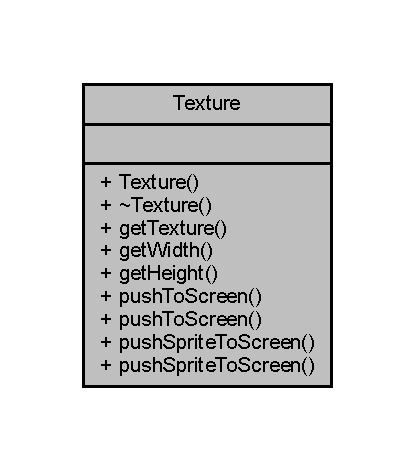
\includegraphics[width=199pt]{class_texture__coll__graph}
\end{center}
\end{figure}
\subsection*{Public Member Functions}
\begin{DoxyCompactItemize}
\item 
\hyperlink{class_texture_a6edf59e3b10e474356e8a7878af56b83}{Texture} (std\+::string, S\+D\+L\+\_\+\+Renderer $\ast$, bool)
\item 
\hyperlink{class_texture_a09c4bcb7462f64c1d20fa69dba3cee8a}{$\sim$\+Texture} ()
\item 
S\+D\+L\+\_\+\+Texture $\ast$ \hyperlink{class_texture_a77a1ae0043a4b318a60df3b02ef2d3f6}{get\+Texture} ()
\item 
int \hyperlink{class_texture_a91a6fd3355bc870194851514194daaab}{get\+Width} ()
\item 
int \hyperlink{class_texture_a80e143905655b173df5994300088ce35}{get\+Height} ()
\item 
void \hyperlink{class_texture_aec498f1f84eb10bb60d3c3117884e70f}{push\+To\+Screen} (S\+D\+L\+\_\+\+Renderer $\ast$, int, int)
\item 
void \hyperlink{class_texture_ab3b1f6aa29a50ef2c012fbc9d0cb8bd8}{push\+To\+Screen} (S\+D\+L\+\_\+\+Renderer $\ast$, int, int, int, int)
\item 
void \hyperlink{class_texture_a703db8963b46b751b8affce1807725b7}{push\+Sprite\+To\+Screen} (S\+D\+L\+\_\+\+Renderer $\ast$, int, int, int, int, int, int)
\item 
void \hyperlink{class_texture_a105a3aba66afb7d223ac086aa465b70d}{push\+Sprite\+To\+Screen} (S\+D\+L\+\_\+\+Renderer $\ast$, int, int, int, int, int, int, int, int)
\end{DoxyCompactItemize}


\subsection{Detailed Description}
Creates a \hyperlink{class_texture}{Texture} for use with a renderer Creates a \hyperlink{class_texture}{Texture} from an image file, this can then be used with a renderer. 

\subsection{Constructor \& Destructor Documentation}
\hypertarget{class_texture_a6edf59e3b10e474356e8a7878af56b83}{\index{Texture@{Texture}!Texture@{Texture}}
\index{Texture@{Texture}!Texture@{Texture}}
\subsubsection[{Texture}]{\setlength{\rightskip}{0pt plus 5cm}Texture\+::\+Texture (
\begin{DoxyParamCaption}
\item[{std\+::string}]{file\+Name, }
\item[{S\+D\+L\+\_\+\+Renderer $\ast$}]{renderer, }
\item[{bool}]{magenta\+Alpha}
\end{DoxyParamCaption}
)}}\label{class_texture_a6edf59e3b10e474356e8a7878af56b83}
Constructs a \hyperlink{class_texture}{Texture} Creates a \hyperlink{class_texture}{Texture} using an image location and a renderer. The magenta pixels of this image can represent alpha if needed. 
\begin{DoxyParams}{Parameters}
{\em std\+::string} & The location of the image file. \\
\hline
{\em S\+D\+L\+\_\+\+Renderer$\ast$} & The renderer. \\
\hline
{\em bool} & If true any magenta pixels in the image will be converted to alpha \\
\hline
\end{DoxyParams}
\hypertarget{class_texture_a09c4bcb7462f64c1d20fa69dba3cee8a}{\index{Texture@{Texture}!````~Texture@{$\sim$\+Texture}}
\index{````~Texture@{$\sim$\+Texture}!Texture@{Texture}}
\subsubsection[{$\sim$\+Texture}]{\setlength{\rightskip}{0pt plus 5cm}Texture\+::$\sim$\+Texture (
\begin{DoxyParamCaption}
{}
\end{DoxyParamCaption}
)}}\label{class_texture_a09c4bcb7462f64c1d20fa69dba3cee8a}
De-\/constructs a \hyperlink{class_texture}{Texture} De-\/constructs the \hyperlink{class_texture}{Texture} deleting the \hyperlink{class_texture}{Texture} from memory. 

\subsection{Member Function Documentation}
\hypertarget{class_texture_a80e143905655b173df5994300088ce35}{\index{Texture@{Texture}!get\+Height@{get\+Height}}
\index{get\+Height@{get\+Height}!Texture@{Texture}}
\subsubsection[{get\+Height}]{\setlength{\rightskip}{0pt plus 5cm}int Texture\+::get\+Height (
\begin{DoxyParamCaption}
{}
\end{DoxyParamCaption}
)}}\label{class_texture_a80e143905655b173df5994300088ce35}
Getter \# Returns texture\+Height \begin{DoxyReturn}{Returns}
the value of texture\+Height. 
\end{DoxyReturn}
\hypertarget{class_texture_a77a1ae0043a4b318a60df3b02ef2d3f6}{\index{Texture@{Texture}!get\+Texture@{get\+Texture}}
\index{get\+Texture@{get\+Texture}!Texture@{Texture}}
\subsubsection[{get\+Texture}]{\setlength{\rightskip}{0pt plus 5cm}S\+D\+L\+\_\+\+Texture $\ast$ Texture\+::get\+Texture (
\begin{DoxyParamCaption}
{}
\end{DoxyParamCaption}
)}}\label{class_texture_a77a1ae0043a4b318a60df3b02ef2d3f6}
Getter \# Returns a pointer to the \hyperlink{class_texture}{Texture} \begin{DoxyReturn}{Returns}
a pointer to the \hyperlink{class_texture}{Texture} data. 
\end{DoxyReturn}
\hypertarget{class_texture_a91a6fd3355bc870194851514194daaab}{\index{Texture@{Texture}!get\+Width@{get\+Width}}
\index{get\+Width@{get\+Width}!Texture@{Texture}}
\subsubsection[{get\+Width}]{\setlength{\rightskip}{0pt plus 5cm}int Texture\+::get\+Width (
\begin{DoxyParamCaption}
{}
\end{DoxyParamCaption}
)}}\label{class_texture_a91a6fd3355bc870194851514194daaab}
Getter \# Returns texture\+Width \begin{DoxyReturn}{Returns}
the value of texture\+Width. 
\end{DoxyReturn}
\hypertarget{class_texture_a703db8963b46b751b8affce1807725b7}{\index{Texture@{Texture}!push\+Sprite\+To\+Screen@{push\+Sprite\+To\+Screen}}
\index{push\+Sprite\+To\+Screen@{push\+Sprite\+To\+Screen}!Texture@{Texture}}
\subsubsection[{push\+Sprite\+To\+Screen}]{\setlength{\rightskip}{0pt plus 5cm}void Texture\+::push\+Sprite\+To\+Screen (
\begin{DoxyParamCaption}
\item[{S\+D\+L\+\_\+\+Renderer $\ast$}]{renderer, }
\item[{int}]{x, }
\item[{int}]{y, }
\item[{int}]{src\+X, }
\item[{int}]{src\+Y, }
\item[{int}]{src\+Width, }
\item[{int}]{src\+Height}
\end{DoxyParamCaption}
)}}\label{class_texture_a703db8963b46b751b8affce1807725b7}
Pushes the image to the Renderer, to the X\+Y Coordinates. Only displays the source rectangle inputed. 
\begin{DoxyParams}{Parameters}
{\em S\+D\+L\+\_\+\+Renderer$\ast$} & The renderer. \\
\hline
{\em int} & x coordinate of the image. \\
\hline
{\em int} & y coordinate of the image. \\
\hline
{\em int} & x coordinate of the source image. \\
\hline
{\em int} & y coordinate of the source image. \\
\hline
{\em int} & width of the source image. \\
\hline
{\em int} & height of the source image. \\
\hline
\end{DoxyParams}


Here is the caller graph for this function\+:
\nopagebreak
\begin{figure}[H]
\begin{center}
\leavevmode
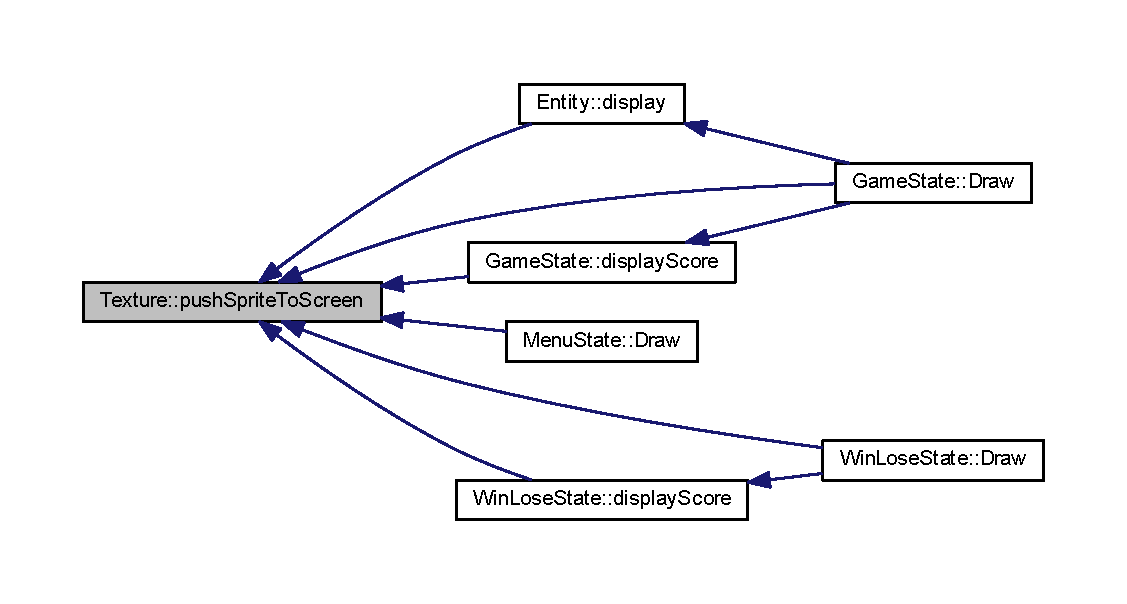
\includegraphics[width=350pt]{class_texture_a703db8963b46b751b8affce1807725b7_icgraph}
\end{center}
\end{figure}


\hypertarget{class_texture_a105a3aba66afb7d223ac086aa465b70d}{\index{Texture@{Texture}!push\+Sprite\+To\+Screen@{push\+Sprite\+To\+Screen}}
\index{push\+Sprite\+To\+Screen@{push\+Sprite\+To\+Screen}!Texture@{Texture}}
\subsubsection[{push\+Sprite\+To\+Screen}]{\setlength{\rightskip}{0pt plus 5cm}void Texture\+::push\+Sprite\+To\+Screen (
\begin{DoxyParamCaption}
\item[{S\+D\+L\+\_\+\+Renderer $\ast$}]{renderer, }
\item[{int}]{x, }
\item[{int}]{y, }
\item[{int}]{src\+X, }
\item[{int}]{src\+Y, }
\item[{int}]{src\+Width, }
\item[{int}]{src\+Height, }
\item[{int}]{width, }
\item[{int}]{height}
\end{DoxyParamCaption}
)}}\label{class_texture_a105a3aba66afb7d223ac086aa465b70d}
Pushes the image to the Renderer, to the X\+Y Coordinates. Only displays the source rectangle inputed. This is scaled to the width and height inputed. 
\begin{DoxyParams}{Parameters}
{\em S\+D\+L\+\_\+\+Renderer$\ast$} & The renderer. \\
\hline
{\em int} & x coordinate of the image. \\
\hline
{\em int} & y coordinate of the image. \\
\hline
{\em int} & x coordinate of the source image. \\
\hline
{\em int} & y coordinate of the source image. \\
\hline
{\em int} & width of the source image. \\
\hline
{\em int} & height of the source image. \\
\hline
{\em int} & width of the scaled image. \\
\hline
{\em int} & height of the scaled image. \\
\hline
\end{DoxyParams}
\hypertarget{class_texture_aec498f1f84eb10bb60d3c3117884e70f}{\index{Texture@{Texture}!push\+To\+Screen@{push\+To\+Screen}}
\index{push\+To\+Screen@{push\+To\+Screen}!Texture@{Texture}}
\subsubsection[{push\+To\+Screen}]{\setlength{\rightskip}{0pt plus 5cm}void Texture\+::push\+To\+Screen (
\begin{DoxyParamCaption}
\item[{S\+D\+L\+\_\+\+Renderer $\ast$}]{renderer, }
\item[{int}]{x, }
\item[{int}]{y}
\end{DoxyParamCaption}
)}}\label{class_texture_aec498f1f84eb10bb60d3c3117884e70f}
Pushes the image to the Renderer, to the X\+Y Coordinates. 
\begin{DoxyParams}{Parameters}
{\em S\+D\+L\+\_\+\+Renderer$\ast$} & The renderer. \\
\hline
{\em int} & x coordinate of the image. \\
\hline
{\em int} & y coordinate of the image. \\
\hline
\end{DoxyParams}


Here is the caller graph for this function\+:
\nopagebreak
\begin{figure}[H]
\begin{center}
\leavevmode
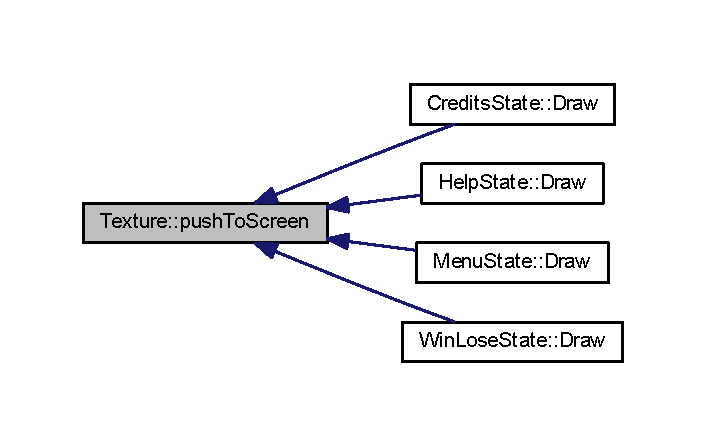
\includegraphics[width=339pt]{class_texture_aec498f1f84eb10bb60d3c3117884e70f_icgraph}
\end{center}
\end{figure}


\hypertarget{class_texture_ab3b1f6aa29a50ef2c012fbc9d0cb8bd8}{\index{Texture@{Texture}!push\+To\+Screen@{push\+To\+Screen}}
\index{push\+To\+Screen@{push\+To\+Screen}!Texture@{Texture}}
\subsubsection[{push\+To\+Screen}]{\setlength{\rightskip}{0pt plus 5cm}void Texture\+::push\+To\+Screen (
\begin{DoxyParamCaption}
\item[{S\+D\+L\+\_\+\+Renderer $\ast$}]{renderer, }
\item[{int}]{x, }
\item[{int}]{y, }
\item[{int}]{width, }
\item[{int}]{height}
\end{DoxyParamCaption}
)}}\label{class_texture_ab3b1f6aa29a50ef2c012fbc9d0cb8bd8}
Pushes the image to the Renderer, to the X\+Y Coordinates. This is scaled to the width and height inputed. 
\begin{DoxyParams}{Parameters}
{\em S\+D\+L\+\_\+\+Renderer$\ast$} & The renderer. \\
\hline
{\em int} & x coordinate of the image. \\
\hline
{\em int} & y coordinate of the image. \\
\hline
{\em int} & width of the scaled image. \\
\hline
{\em int} & height of the scaled image. \\
\hline
\end{DoxyParams}


The documentation for this class was generated from the following files\+:\begin{DoxyCompactItemize}
\item 
P\+G\+G\+Assignment1\+S\+D\+L/texture.\+h\item 
P\+G\+G\+Assignment1\+S\+D\+L/texture.\+cpp\end{DoxyCompactItemize}

\hypertarget{class_win_lose_state}{\section{Win\+Lose\+State Class Reference}
\label{class_win_lose_state}\index{Win\+Lose\+State@{Win\+Lose\+State}}
}


Creates a \hyperlink{class_win_lose_state}{Win\+Lose\+State} object. Creates a \hyperlink{class_win_lose_state}{Win\+Lose\+State} object that inherits \hyperlink{class_state}{State}.  




{\ttfamily \#include $<$win\+Lose\+State.\+h$>$}



Inheritance diagram for Win\+Lose\+State\+:
\nopagebreak
\begin{figure}[H]
\begin{center}
\leavevmode
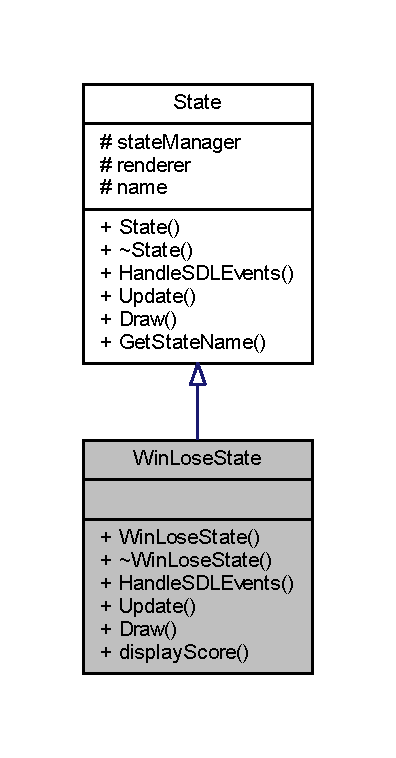
\includegraphics[width=190pt]{class_win_lose_state__inherit__graph}
\end{center}
\end{figure}


Collaboration diagram for Win\+Lose\+State\+:
\nopagebreak
\begin{figure}[H]
\begin{center}
\leavevmode
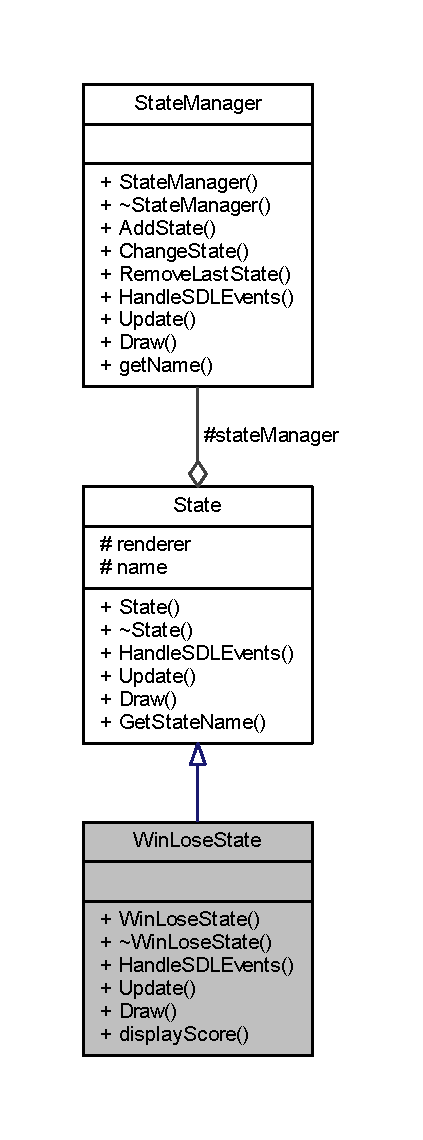
\includegraphics[width=203pt]{class_win_lose_state__coll__graph}
\end{center}
\end{figure}
\subsection*{Public Member Functions}
\begin{DoxyCompactItemize}
\item 
\hyperlink{class_win_lose_state_a047ccdc0cc156d65c076eb845398ef84}{Win\+Lose\+State} (\hyperlink{class_state_manager}{State\+Manager} $\ast$, S\+D\+L\+\_\+\+Renderer $\ast$, bool, int)
\item 
\hyperlink{class_win_lose_state_ac7ee2a9515081ba03b96cb78c5837d72}{$\sim$\+Win\+Lose\+State} ()
\item 
bool \hyperlink{class_win_lose_state_ada8c41baa8011df1aeae4b7b0d9b00f8}{Handle\+S\+D\+L\+Events} ()
\item 
void \hyperlink{class_win_lose_state_a98e675ce31aa41ad95ba36fd9e77dde6}{Update} (float delta\+Time)
\item 
void \hyperlink{class_win_lose_state_a862a5bb9422480b36671acb21cc987ba}{Draw} ()
\item 
void \hyperlink{class_win_lose_state_af7a44a05cae2f79731b9e36ea1ef4f7e}{display\+Score} ()
\end{DoxyCompactItemize}
\subsection*{Additional Inherited Members}


\subsection{Detailed Description}
Creates a \hyperlink{class_win_lose_state}{Win\+Lose\+State} object. Creates a \hyperlink{class_win_lose_state}{Win\+Lose\+State} object that inherits \hyperlink{class_state}{State}. 

\subsection{Constructor \& Destructor Documentation}
\hypertarget{class_win_lose_state_a047ccdc0cc156d65c076eb845398ef84}{\index{Win\+Lose\+State@{Win\+Lose\+State}!Win\+Lose\+State@{Win\+Lose\+State}}
\index{Win\+Lose\+State@{Win\+Lose\+State}!Win\+Lose\+State@{Win\+Lose\+State}}
\subsubsection[{Win\+Lose\+State}]{\setlength{\rightskip}{0pt plus 5cm}Win\+Lose\+State\+::\+Win\+Lose\+State (
\begin{DoxyParamCaption}
\item[{{\bf State\+Manager} $\ast$}]{in\+State\+Manager, }
\item[{S\+D\+L\+\_\+\+Renderer $\ast$}]{in\+Renderer, }
\item[{bool}]{in\+Win, }
\item[{int}]{in\+Score}
\end{DoxyParamCaption}
)}}\label{class_win_lose_state_a047ccdc0cc156d65c076eb845398ef84}
Constructs a \hyperlink{class_win_lose_state}{Win\+Lose\+State} object Constructs a \hyperlink{class_win_lose_state}{Win\+Lose\+State} object 
\begin{DoxyParams}{Parameters}
{\em \hyperlink{class_state_manager}{State\+Manager}} & $\ast$ a pointer to the \hyperlink{class_state_manager}{State\+Manager} \\
\hline
{\em S\+D\+L\+\_\+\+Renderer} & $\ast$ a pointer to the renderer in use. \\
\hline
{\em bool} & if the player won or not \\
\hline
{\em int} & the players score \\
\hline
\end{DoxyParams}


Here is the call graph for this function\+:
\nopagebreak
\begin{figure}[H]
\begin{center}
\leavevmode
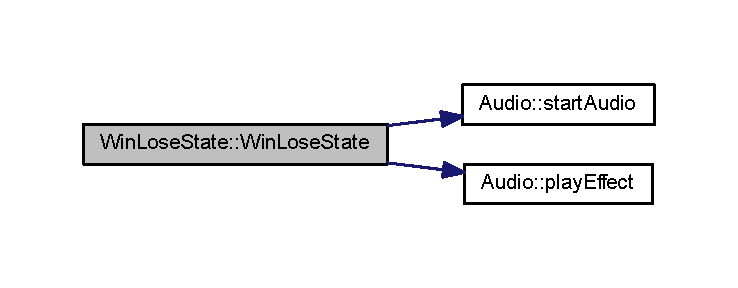
\includegraphics[width=350pt]{class_win_lose_state_a047ccdc0cc156d65c076eb845398ef84_cgraph}
\end{center}
\end{figure}


\hypertarget{class_win_lose_state_ac7ee2a9515081ba03b96cb78c5837d72}{\index{Win\+Lose\+State@{Win\+Lose\+State}!````~Win\+Lose\+State@{$\sim$\+Win\+Lose\+State}}
\index{````~Win\+Lose\+State@{$\sim$\+Win\+Lose\+State}!Win\+Lose\+State@{Win\+Lose\+State}}
\subsubsection[{$\sim$\+Win\+Lose\+State}]{\setlength{\rightskip}{0pt plus 5cm}Win\+Lose\+State\+::$\sim$\+Win\+Lose\+State (
\begin{DoxyParamCaption}
{}
\end{DoxyParamCaption}
)}}\label{class_win_lose_state_ac7ee2a9515081ba03b96cb78c5837d72}
De-\/constructs a \hyperlink{class_win_lose_state}{Win\+Lose\+State} object De-\/constructs the \hyperlink{class_win_lose_state}{Win\+Lose\+State} object 

Here is the call graph for this function\+:
\nopagebreak
\begin{figure}[H]
\begin{center}
\leavevmode
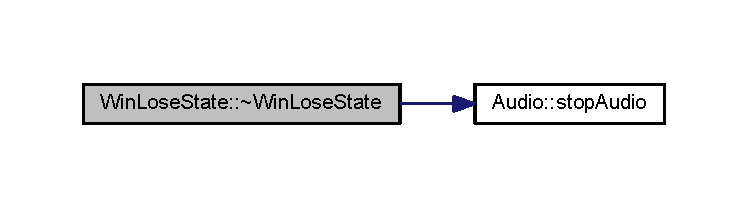
\includegraphics[width=350pt]{class_win_lose_state_ac7ee2a9515081ba03b96cb78c5837d72_cgraph}
\end{center}
\end{figure}




\subsection{Member Function Documentation}
\hypertarget{class_win_lose_state_af7a44a05cae2f79731b9e36ea1ef4f7e}{\index{Win\+Lose\+State@{Win\+Lose\+State}!display\+Score@{display\+Score}}
\index{display\+Score@{display\+Score}!Win\+Lose\+State@{Win\+Lose\+State}}
\subsubsection[{display\+Score}]{\setlength{\rightskip}{0pt plus 5cm}void Win\+Lose\+State\+::display\+Score (
\begin{DoxyParamCaption}
{}
\end{DoxyParamCaption}
)}}\label{class_win_lose_state_af7a44a05cae2f79731b9e36ea1ef4f7e}
A function to draw the score to the screen A function to draw the score to the screen using the renderer 

Here is the call graph for this function\+:
\nopagebreak
\begin{figure}[H]
\begin{center}
\leavevmode
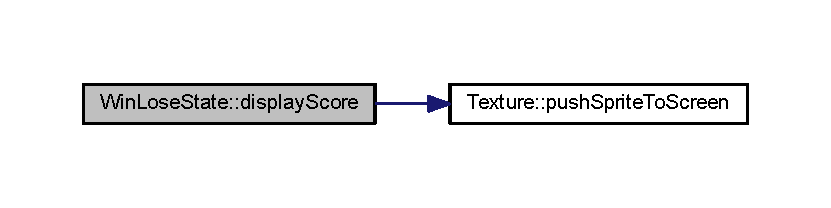
\includegraphics[width=350pt]{class_win_lose_state_af7a44a05cae2f79731b9e36ea1ef4f7e_cgraph}
\end{center}
\end{figure}




Here is the caller graph for this function\+:
\nopagebreak
\begin{figure}[H]
\begin{center}
\leavevmode
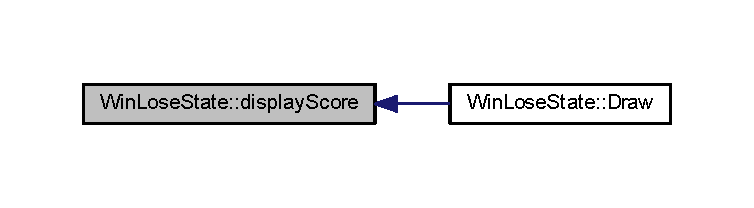
\includegraphics[width=350pt]{class_win_lose_state_af7a44a05cae2f79731b9e36ea1ef4f7e_icgraph}
\end{center}
\end{figure}


\hypertarget{class_win_lose_state_a862a5bb9422480b36671acb21cc987ba}{\index{Win\+Lose\+State@{Win\+Lose\+State}!Draw@{Draw}}
\index{Draw@{Draw}!Win\+Lose\+State@{Win\+Lose\+State}}
\subsubsection[{Draw}]{\setlength{\rightskip}{0pt plus 5cm}void Win\+Lose\+State\+::\+Draw (
\begin{DoxyParamCaption}
{}
\end{DoxyParamCaption}
)\hspace{0.3cm}{\ttfamily [virtual]}}}\label{class_win_lose_state_a862a5bb9422480b36671acb21cc987ba}
A function to draw to the screen A function to draw to the screen using the renderer 

Implements \hyperlink{class_state_a8b0cdb0e7450a9bb3580a33dfbe4d981}{State}.



Here is the call graph for this function\+:
\nopagebreak
\begin{figure}[H]
\begin{center}
\leavevmode
\includegraphics[width=350pt]{class_win_lose_state_a862a5bb9422480b36671acb21cc987ba_cgraph}
\end{center}
\end{figure}


\hypertarget{class_win_lose_state_ada8c41baa8011df1aeae4b7b0d9b00f8}{\index{Win\+Lose\+State@{Win\+Lose\+State}!Handle\+S\+D\+L\+Events@{Handle\+S\+D\+L\+Events}}
\index{Handle\+S\+D\+L\+Events@{Handle\+S\+D\+L\+Events}!Win\+Lose\+State@{Win\+Lose\+State}}
\subsubsection[{Handle\+S\+D\+L\+Events}]{\setlength{\rightskip}{0pt plus 5cm}bool Win\+Lose\+State\+::\+Handle\+S\+D\+L\+Events (
\begin{DoxyParamCaption}
{}
\end{DoxyParamCaption}
)\hspace{0.3cm}{\ttfamily [virtual]}}}\label{class_win_lose_state_ada8c41baa8011df1aeae4b7b0d9b00f8}
A function to handle the S\+D\+L events A function to handle the S\+D\+L events for use with the \hyperlink{class_win_lose_state}{Win\+Lose\+State} \begin{DoxyReturn}{Returns}
bool if false then quit \hyperlink{class_win_lose_state}{Win\+Lose\+State} 
\end{DoxyReturn}


Implements \hyperlink{class_state_a648d9182cab9aeb914ef778f94e2b437}{State}.



Here is the call graph for this function\+:
\nopagebreak
\begin{figure}[H]
\begin{center}
\leavevmode
\includegraphics[width=350pt]{class_win_lose_state_ada8c41baa8011df1aeae4b7b0d9b00f8_cgraph}
\end{center}
\end{figure}


\hypertarget{class_win_lose_state_a98e675ce31aa41ad95ba36fd9e77dde6}{\index{Win\+Lose\+State@{Win\+Lose\+State}!Update@{Update}}
\index{Update@{Update}!Win\+Lose\+State@{Win\+Lose\+State}}
\subsubsection[{Update}]{\setlength{\rightskip}{0pt plus 5cm}void Win\+Lose\+State\+::\+Update (
\begin{DoxyParamCaption}
\item[{float}]{delta\+Time}
\end{DoxyParamCaption}
)\hspace{0.3cm}{\ttfamily [virtual]}}}\label{class_win_lose_state_a98e675ce31aa41ad95ba36fd9e77dde6}
A function to update the \hyperlink{class_win_lose_state}{Win\+Lose\+State} A function to update the \hyperlink{class_win_lose_state}{Win\+Lose\+State} to allow the \hyperlink{class_win_lose_state}{Win\+Lose\+State} to run 
\begin{DoxyParams}{Parameters}
{\em float} & the delta time \\
\hline
\end{DoxyParams}


Implements \hyperlink{class_state_a770f40188fdfc64bc95a5166fef12e02}{State}.



Here is the call graph for this function\+:
\nopagebreak
\begin{figure}[H]
\begin{center}
\leavevmode
\includegraphics[width=323pt]{class_win_lose_state_a98e675ce31aa41ad95ba36fd9e77dde6_cgraph}
\end{center}
\end{figure}




The documentation for this class was generated from the following files\+:\begin{DoxyCompactItemize}
\item 
P\+G\+G\+Assignment1\+S\+D\+L/win\+Lose\+State.\+h\item 
P\+G\+G\+Assignment1\+S\+D\+L/win\+Lose\+State.\+cpp\end{DoxyCompactItemize}

%--- End generated contents ---

% Index
\newpage
\phantomsection
\addcontentsline{toc}{chapter}{Index}
\printindex

\end{document}
